% Options for packages loaded elsewhere
\PassOptionsToPackage{unicode}{hyperref}
\PassOptionsToPackage{hyphens}{url}
%
\documentclass[
]{article}
\usepackage{amsmath,amssymb}
\usepackage{iftex}
\ifPDFTeX
  \usepackage[T1]{fontenc}
  \usepackage[utf8]{inputenc}
  \usepackage{textcomp} % provide euro and other symbols
\else % if luatex or xetex
  \usepackage{unicode-math} % this also loads fontspec
  \defaultfontfeatures{Scale=MatchLowercase}
  \defaultfontfeatures[\rmfamily]{Ligatures=TeX,Scale=1}
\fi
\usepackage{lmodern}
\ifPDFTeX\else
  % xetex/luatex font selection
\fi
% Use upquote if available, for straight quotes in verbatim environments
\IfFileExists{upquote.sty}{\usepackage{upquote}}{}
\IfFileExists{microtype.sty}{% use microtype if available
  \usepackage[]{microtype}
  \UseMicrotypeSet[protrusion]{basicmath} % disable protrusion for tt fonts
}{}
\makeatletter
\@ifundefined{KOMAClassName}{% if non-KOMA class
  \IfFileExists{parskip.sty}{%
    \usepackage{parskip}
  }{% else
    \setlength{\parindent}{0pt}
    \setlength{\parskip}{6pt plus 2pt minus 1pt}}
}{% if KOMA class
  \KOMAoptions{parskip=half}}
\makeatother
\usepackage{xcolor}
\usepackage[margin=1in]{geometry}
\usepackage{longtable,booktabs,array}
\usepackage{calc} % for calculating minipage widths
% Correct order of tables after \paragraph or \subparagraph
\usepackage{etoolbox}
\makeatletter
\patchcmd\longtable{\par}{\if@noskipsec\mbox{}\fi\par}{}{}
\makeatother
% Allow footnotes in longtable head/foot
\IfFileExists{footnotehyper.sty}{\usepackage{footnotehyper}}{\usepackage{footnote}}
\makesavenoteenv{longtable}
\usepackage{graphicx}
\makeatletter
\newsavebox\pandoc@box
\newcommand*\pandocbounded[1]{% scales image to fit in text height/width
  \sbox\pandoc@box{#1}%
  \Gscale@div\@tempa{\textheight}{\dimexpr\ht\pandoc@box+\dp\pandoc@box\relax}%
  \Gscale@div\@tempb{\linewidth}{\wd\pandoc@box}%
  \ifdim\@tempb\p@<\@tempa\p@\let\@tempa\@tempb\fi% select the smaller of both
  \ifdim\@tempa\p@<\p@\scalebox{\@tempa}{\usebox\pandoc@box}%
  \else\usebox{\pandoc@box}%
  \fi%
}
% Set default figure placement to htbp
\def\fps@figure{htbp}
\makeatother
\setlength{\emergencystretch}{3em} % prevent overfull lines
\providecommand{\tightlist}{%
  \setlength{\itemsep}{0pt}\setlength{\parskip}{0pt}}
\setcounter{secnumdepth}{-\maxdimen} % remove section numbering
\usepackage{multicol}
\usepackage{longtable}
\setlength{\columnsep}{1cm}
\usepackage{enumitem}
\usepackage{booktabs}
\usepackage{array}
\usepackage{float}
\usepackage{longtable}
\usepackage{multirow}
\usepackage{wrapfig}
\usepackage{colortbl}
\usepackage{pdflscape}
\usepackage{tabu}
\usepackage{threeparttable}
\usepackage{threeparttablex}
\usepackage[normalem]{ulem}
\usepackage{makecell}
\usepackage{xcolor}
\usepackage{bookmark}
\IfFileExists{xurl.sty}{\usepackage{xurl}}{} % add URL line breaks if available
\urlstyle{same}
\hypersetup{
  pdftitle={Análisis de Variables que Influyen en la Inversión, Innovación e Implementación de la Inteligencia Artificial},
  hidelinks,
  pdfcreator={LaTeX via pandoc}}

\title{Análisis de Variables que Influyen en la Inversión, Innovación e
Implementación de la Inteligencia Artificial}
\author{Adrada Isabel, De la Peña Juan, Terán Federico, Troncoso
Samuel\\
Pontificia Universidad Javeriana Cali}
\date{}

\begin{document}
\maketitle

\begin{multicols}{2}

\section{Resumen}
Este estudio analiza las variables clave que influyen en la inversión, innovación e implementación de la inteligencia artificial (IA) a nivel global, utilizando el AI Global Index como referencia. Mediante un análisis estadístico descriptivo y correlacional, se identificaron los índices Commerce (inversión), Research (innovación) y Talent (implementación) como factores críticos, destacando su relación lineal significativa con el Total Score. Además, se exploró el impacto de la variable Región en la distribución geográfica del desarrollo de IA.

\section{Key words}
Inteligencia artificial, inversión, innovación, implementación, análisis estadístico.

\section{Introducción}
Las compañıas involucradas en el desarrollo tecnológico con inteligencia artificial (IA) necesitan identificar las regiones con mayor potencial de adopción e implementación de estas herramientas. Este análisis es crucial para la definición de mercados objetivo y la planificación de estrategias de expansión geográfica, razón por lo cuál, debido a la incertidumbre respecto a los factores con mayor impacto en el potencial éxito de los planes de expansión operativa en diferentes partes del mundo, se plantea el interrogante ¿Qué variables tienen mayor influencia en los niveles de inversión, innovación e implementación de la inteligencia artificial según lo reflejado en el AI Global Index [1] (índice que compara diferentes países en estos niveles), y cómo varía esta influencia según la región geográfica?

El objetivo general de este estudio radica en identificar las variables con un mayor grado de influencia en el nivel de inversión, innovación e implementación de la inteligencia artificial, reflejado en el AI global index de diferentes regiones del mundo, por lo cuál, en primera instancia se identificaron los índices para cada factor mencionado con un mayor coeficiente de correlación lineal de Pearson de acuerdo a la metodología e interpretación plaenteada por Navidi [2], permitiendo el plateamiento de los objetivos específicos:

\begin{itemize}
\item Determinar la influencia de los factores relacionados con la inversión mediante el índice Commerce en el desarrollo de la IA.
\item Determinar la influencia de los factores relacionados con la innovación mediante el índice Research en el desarrollo de la IA.
\item Determinar la influencia de los factores relacionados con la implementación mediante el índice Talent en el desarrollo de la IA.
\item Determinar la influencia de la ubicación geográfica en el desarrollo de la IA mediante la categorización por Región.
\end{itemize}

En primera instancia y considerando que el índice Research tiene la más alta correlación lineal con Total Score de las variables presentadas, se formula la siguiente hipótesis: la media del índice Research es $≤$ a 20 puntos (teniendo en cuenta que el puntaje regional más alto de Research es 20.72).

Por otro lado, al contemplar las diferencias regionales para la resolución de la pregunta problema de este estudio, se plantea la siguiente hipótesis: por lo menos el 80\% de los datos con un Total Score $≥$ a 5 son parte de la región Africa (al tener en cuenta que la región Africa tiene los algunos de los puntajes más bajos para las diferentes variables).

Finalmente, con el propósito de realizar una comparación regional para determinar cuáles son las zonas con mayor potencial de desarrollo en IA se plantea la siguiente hipótesis sobre dos grupos regionales: el puntaje medio del índice Total Score en Europe es mayor a el promedio de Total Score en Estados Unidos (considerando que en múltiples sectores se considera a Europa y Estados Unidos como regiones altamente desarrolladas).




\section{Metodología}

Para la realización de este estudio, es necesario definir la población y muestra a estudiar además de la realización de una revisión preliminar de las variables presentadas en la base de datos AI global Index, una presentación de los datos incluyendo los países que conforman las regiones estudiadas, la relación lineal entre las diferentes variables a través de gráficos de disperción y el coeficiente de correlación lineal de Pearson (criterio utilizado para la definición de las variables a estudiar a través de los objetivos específicos) y medidas de tendencia central, posición y disperción de los datos.

La población considerada para este estudio corresponde a todos los países del mundo, mientras la muestra se delimita a los países y regiones incluidas en el AI Global Index con datos completos para los factores inversión, innovación e implementación. La unidad de análisis en este estudio son las 5 regiones conformadas por los 62 países estudiados, evaluado según las variables cuantitativas y cualitativas definidas en la Tabla 1. 

Para la definición de las variables a estudiar a partir de la base de datos AI Global Index trabajada en el presente estudio, se relalizó una exploración preliminar de los datos en la Tabla 1, donde se nombran las variables, se clasifican como cualitativas o cuantitativas, se categorizan como continuas o discretas, o nominal u ordinal según el caso y se realiza una descripción de las mismas.\\


\end{multicols}

\renewcommand{\arraystretch}{1.5}
\begin{footnotesize}
\begin{longtable}[t]{lllp{8cm}}
\caption{\label{tab:tabla1}Variables y su clasificación}\\
\toprule
Variable & Clasificación & Categorización & Descripción\\
\midrule
Country & Cualitativa & Nominal & Nombre del país donde se evalúa el AI Global Index.\\
Talent & Cuantitativa & Continua & Indicador de disponibilidad de profesionales calificados para la provisión de soluciones de inteligencia artificial.\\
Infraestructure & Cuantitativa & Continua & Indicador de fiabilidad y la escala de la infraestructura de acceso, desde la electricidad e Internet, hasta las capacidades de superintarmética.\\
Operating Enviroment & Cuantitativa & Continua & Indicador del contexto regulatorio y la opinión pública en torno a la inteligencia artificial.\\
Research & Cuantitativa & Continua & Indicador del alcance de la investigación especializada y los investigadores; investigando la cantidad de publicaciones y citas en revistas académicas creíbles.\\
\addlinespace
Development & Cuantitativa & Continua & Indicador de desarrollo de plataformas y algoritmos fundamentales en los que se basan los proyectos innovadores de inteligencia artificial.\\
Government Strategy & Cuantitativa & Continua & Indicador de la profundidad del compromiso del gobierno nacional con la inteligencia artificial; investigando los compromisos de gasto y las estrategias nacionales.\\
Commerce & Cuantitativa & Continua & Indicador del nivel de actividad de puesta en marcha, inversión e iniciativas comerciales basadas en la inteligencia artificial.\\
Total Score & Cuantitativa & Continua & Indicador AI Global Index que compara a las naciones en su nivel de inversión, innovación e implementación de la inteligencia artificial.\\
Region & Cualitativa & Nominal & Agrupacion de países según su localización geográfica en regiones.\\
\addlinespace
Cluster & Cualitativa & Nominal & Agrupación de países según su historia de incursión en el desarrollo de tecnología relacionada con la Inteligencia Artificial.\\
Income Group & Cualitativa & Ordinal & Nivel de ingresos presentado en el país.\\
Political Regime & Cualitativa & Nominal & Tipo de régimen político presentado en el país.\\
\bottomrule
\end{longtable}

\end{footnotesize}\renewcommand{\arraystretch}{1}

\begin{multicols}{2}

En la Tabla 2 se presenta la consitución de la unidad de análisis de este estudio; cada una de las 5 regiones con los países que las conforman (para un total de 62 países a nivel mundial) con el fin de proporcionar claridad sobre la proveniencia de los datos regionales que se presentan en este informe, ya que los datos referentes a las regiones no abarcan la totalidad de los países pertenecientes a las mismas y las regiones están formadas por diferentes cantidades de paises.

\end{multicols}

\renewcommand{\arraystretch}{1.5}
\begin{footnotesize}
\begin{longtable}[t]{lp{12cm}}
\caption{\label{tab:tabla2}Países agrupados por región}\\
\toprule
Región & Países\\
\midrule
Africa & Kenya, Morocco, Nigeria, South Africa, Tunisia\\
Americas & Argentina, Brazil, Canada, Chile, Colombia, Mexico, United States of America, Uruguay\\
Asia-Pacific & Australia, China, Hong Kong, India, Indonesia, Japan, Malaysia, New Zealand, Pakistan, Singapore, South Korea, Sri Lanka, Taiwan, Vietnam\\
Europe & Armenia, Austria, Belgium, Czech Republic, Denmark, Estonia, Finland, France, Germany, Greece, Hungary, Iceland, Ireland, Italy, Lithuania, Luxembourg, Malta, Norway, Poland, Portugal, Russia, Slovakia, Slovenia, Spain, Sweden, Switzerland, The Netherlands, Turkey, United Kingdom\\
Middle East & Bahrain, Egypt, Israel, Qatar, Saudi Arabia, United Arab Emirates\\
\bottomrule
\end{longtable}

\end{footnotesize}\renewcommand{\arraystretch}{1}

\begin{multicols}{2}


Posteriormente, con el propósito de indentificar las posibles variables con un mayor grado de influencia en el nivel de inversión, innovación e implementación de la inteligencia artificial, se elaboró la Figura 1, la cuál presenta una comparación de las distribuciones y disperciones de las variables y con respectivos coeficientes de correlación lineal de Pearson con el fin de reconocer los índices que presentan un mayor valor respecto al AI Global Index (Total Score), los cuáles fueron Commerce para el nivel de inversión, Research para la innovación y Talent para la implemetación. 




\begin{center}
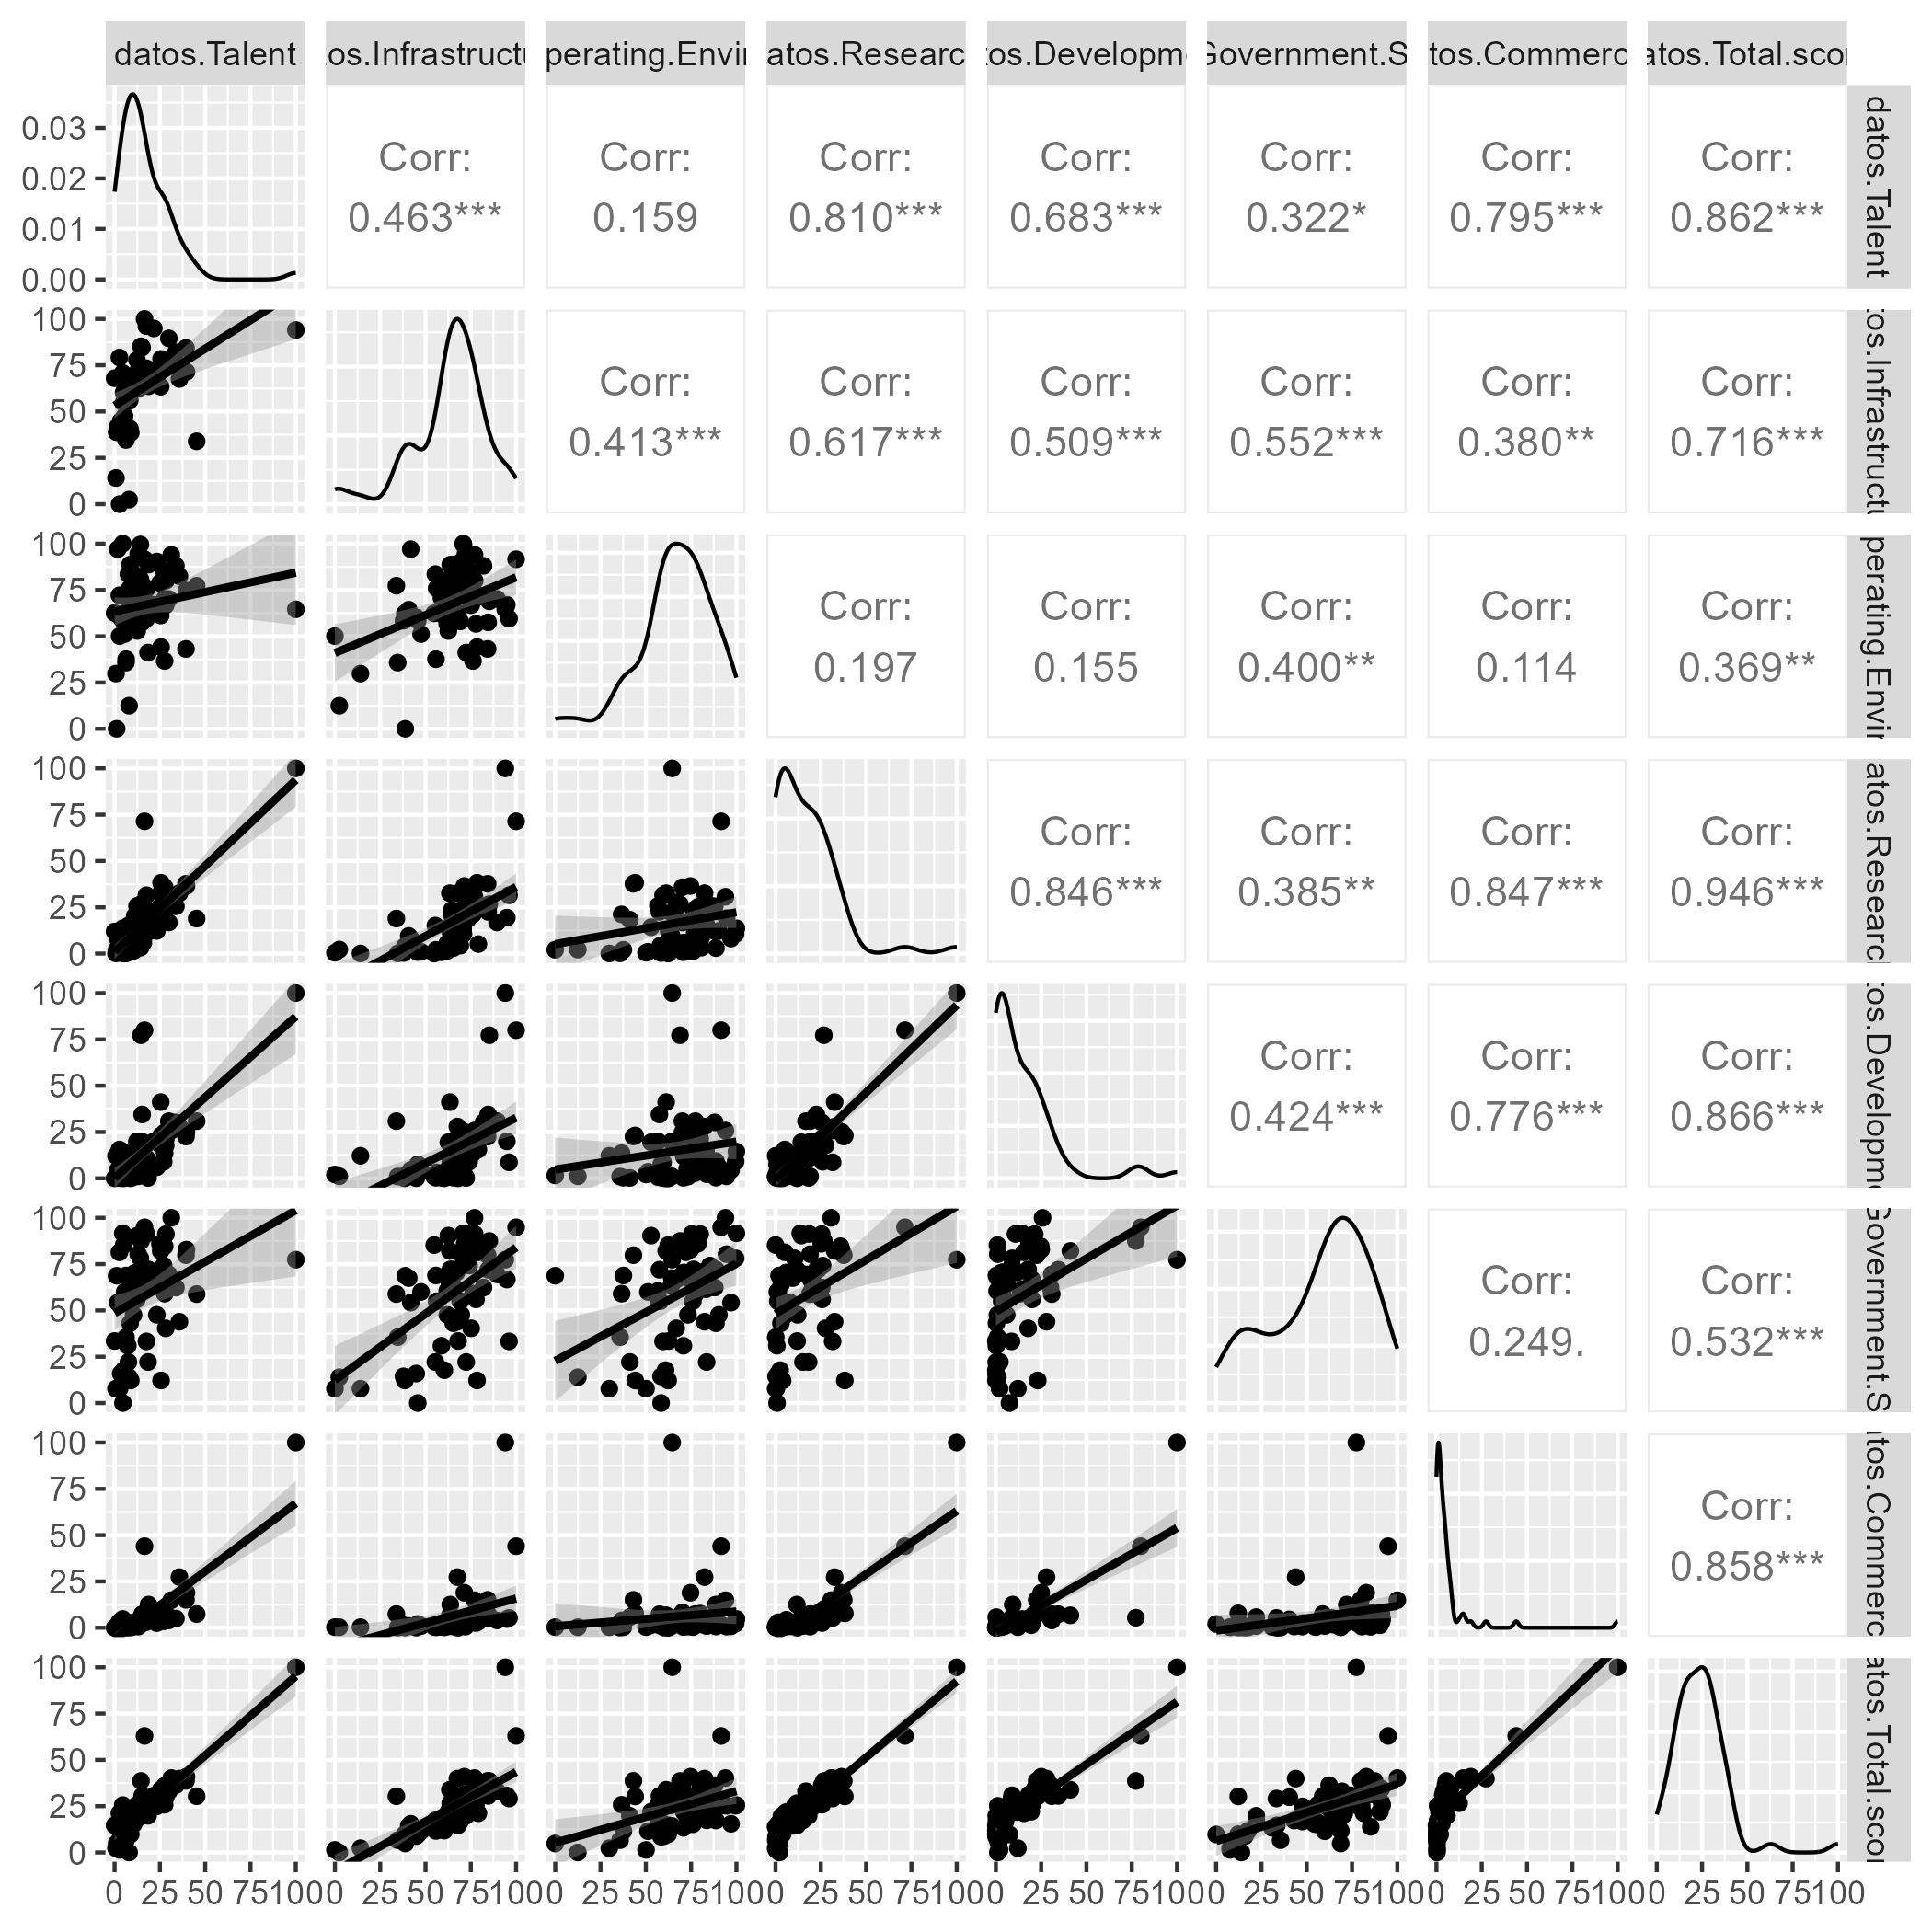
\includegraphics[width=\linewidth]{figura1.png}
\end{center}
Figura 1. Correlación lineal de Pearson índices.

El análisis realizado incluye estadísticas descriptivas: medidas de tendencia central, dispersión y posición, correlación lineal de Pearson entre las variables cuantitativas y el índice total y comparación de medias para evaluar diferencias significativas entre regiones. Posteriormente, se emplearon métodos de análisis multivariado para explorar relaciones más complejas entre las variables, como el análisis de componentes principales (ACP) para identificar patrones latentes en los datos.

Para la realización de las 3 pruebas de hipótesis presentadas en el estudio se realizó un muestreo aleatorio de las poblaciones corrrespondientes mediante la función sample para obtener muestras de 30 datos, asegurando que el tamaño de muestra sea grande (n >= 30) garantizando el cumplimiento del Teorema Central del Límite [3] para la realización de intérvalos de confianza y pruebas de hipótesis con resultados fidedignos.

Finalmente se realizaron dos modelos de regresión lineal, uno simple y uno múltiple, donde mediante el coeficiente de correlación lineal de Pearson, coeficiente de determinación y gráficas de disperción y distribución se generó el modelo, se determinó su bondad y se verificaron los supuestos del mismo.







\section{Resultados}
En la Tabla 3 se presentan las medidas de tendencia central y posición de las variables cuantitativas Índice Commerce, Research y Talent discriminadas de forma regional. 

Para casi todos los casos, la moda presentó más de tres valores, lo cuál no brinda mucha información acerca de los datos. En el caso de la media y mediana en Americas y Middle East, todos los índices difieren drásticamente, lo cuál indica que la distribución de los datos no es normal. En el caso Asia-Pacific, para el indicador Research y Total Score hay una alta cercanía entre los indicadores, planteando la posibilidad de una distribución de campana, sin embargo esto debe ser confirmado gráficamente. Esto mismo ocurre para Europe con todos los indicadores, y en Commerce hay una moda única que también es significativamente cercana a la media y mediana. Finalmente para Africa se presenta una alta cercanía de la mediana y la media en los índices Commerce, Talent y Research.

El mínimo en todas las regiones para todos los ídices es menor a 10, excepto Total Score de Americas con un 13.27, por otro lado, el máximo entre regiones presenta discrepancias más significativas, donde el el caso de Americas el máximo es 100 para todos los índices, en Asia-Pacific todos los máximos se encuentran por encima de 40, mientras en Europe los máximos de todos los índices se ubican en 40.93 o menos, al igual que Middle East. En el caso de Africa, toos los máximos de los indicadores se encuentran por debajo de 10.

\end{multicols}

\renewcommand{\arraystretch}{1.3}
\begin{scriptsize}
\begin{longtable}[t]{llrrrrrrr}
\caption{\label{tab:tabla3}Medidas de tendencia central y posición}\\
\toprule
Región & Índice & Media & Moda & Mínimo & Q1 & Mediana & Q3 & Máximo\\
\midrule
Americas & Commerce & 15.15 & > 3 modas & 0.34 & 0.48 & 1.07 & 5.93 & 100.00\\
Americas & Talent & 22.21 & > 3 modas & 1.72 & 6.70 & 9.48 & 17.91 & 100.00\\
Americas & Research & 18.39 & > 3 modas & 0.00 & 1.12 & 3.16 & 13.75 & 100.00\\
Americas & Total Score & 29.03 & > 3 modas & 13.27 & 14.89 & 15.41 & 24.22 & 100.00\\
Asia-Pacific & Commerce & 7.03 & > 3 modas & 0.09 & 0.70 & 3.92 & 7.16 & 44.02\\
\addlinespace
Asia-Pacific & Talent & 17.58 & > 3 modas & 5.51 & 8.61 & 14.86 & 21.87 & 45.27\\
Asia-Pacific & Research & 20.72 & > 3 modas & 0.12 & 3.02 & 20.72 & 30.30 & 71.42\\
Asia-Pacific & Total Score & 25.79 & > 3 modas & 0.00 & 12.88 & 27.45 & 33.03 & 62.92\\
Europe & Commerce & 4.28 & 3.08 & 0.61 & 1.75 & 3.46 & 4.97 & 18.91\\
Europe & Talent & 18.92 & > 3 modas & 6.69 & 12.46 & 16.97 & 27.07 & 39.65\\
\addlinespace
Europe & Research & 17.86 & > 3 modas & 0.28 & 10.60 & 18.60 & 25.21 & 38.24\\
Europe & Total Score & 25.49 & > 3 modas & 8.49 & 20.31 & 25.52 & 30.73 & 40.93\\
Middle East & Commerce & 5.97 & > 3 modas & 0.00 & 0.26 & 1.77 & 4.35 & 27.33\\
Middle East & Talent & 8.17 & > 3 modas & 0.00 & 1.50 & 3.57 & 4.86 & 35.76\\
Middle East & Research & 11.32 & > 3 modas & 2.08 & 3.18 & 8.54 & 13.21 & 32.63\\
\addlinespace
Middle East & Total Score & 19.66 & > 3 modas & 4.83 & 12.51 & 17.91 & 24.49 & 39.89\\
Africa & Commerce & 0.58 & > 3 modas & 0.10 & 0.15 & 0.31 & 0.33 & 2.03\\
Africa & Talent & 4.08 & > 3 modas & 0.75 & 2.74 & 3.36 & 4.61 & 8.94\\
Africa & Research & 1.34 & > 3 modas & 0.07 & 0.45 & 0.83 & 1.46 & 3.90\\
Africa & Total Score & 6.43 & > 3 modas & 1.38 & 2.30 & 8.87 & 9.71 & 9.87\\
\bottomrule
\end{longtable}

\end{scriptsize}\renewcommand{\arraystretch}{1}

\begin{multicols}{2}

En la Tabla 4 se presentan las medidas de disperción, covarianza y correlación lineal de Pearson con respecto al Total Score (AI Global Index) de las variables cuantitativas Índice Commerce, Research y Talent discriminadas de forma regional. 

Americas presentan los rangos más amplios de todas las regiones que van desde 86.73 en Total Score hasta 100 en Research, para Asia-Pacific, Europe y Middle East, los rangos de los diferentes índices varían alrededor de 20 y 40 indicando menor variablidad de los datos con excepciones de los índices Research y Total Score de Asia-Pacific con 71.30 y  62.92 respectivamente. En el caso de Africa se presentan los rangos más bajos donde todos están por debajo de 10, lo cuál sugiere que los datos en la región se distribuyen de manera compacta.

Con respecto al coeeficiente de variación se puede afirmar que para la mayoría de los casos los datos son heterogéneos al presentar un coeficiente > a 50, sin embargo, el índice Talent y Total Score en Europe presentan variación significativa ya que el CV se encuentra en el rango de 10 a 50.

En el caso de la covarianza, esta es positiva para todas las variables, lo cuál plantea la posibilidad de una relación lineal directa con el índice Total Score. Esto es confirmado con el coeficiente de correlación lineal de Pearson, donde un valor superior a 0.8 indica hay una relación muy significativa, lo cuál es cierto para todos los indicadores en Americas y Middle East, Research en Asia-Pacific, Talent y Research en Europe. Por otro lado, una coeficiente entre 0.6 y 0.8 indica una relación significativa, la cuál está presente en Europe para Commerce y en Africa para Talent y Research.


\end{multicols}

\renewcommand{\arraystretch}{1.3}
\begin{scriptsize}
\begin{longtable}[t]{llrrrrrl}
\caption{\label{tab:tabla4}Medidas de dispersión e indicadores por región e índice}\\
\toprule
Región & Índice & Rango & RIQ & Desv.est & CV & Cov Total Score & Corr Total Score\\
\midrule
Americas & Commerce & 99.66 & 5.45 & 34.63 & 228.58 & 1025.58 & 0.99\\
Americas & Talent & 98.28 & 11.21 & 32.68 & 147.14 & 976.48 & 1.00\\
Americas & Research & 100.00 & 12.63 & 34.50 & 187.60 & 1033.01 & 1.00\\
Americas & Total Score & 86.73 & 9.33 & 30.01 & 103.38 & 900.62 & 1.00\\
Asia-Pacific & Commerce & 43.93 & 6.46 & 11.43 & 162.59 & 154.14 & 0.84\\
\addlinespace
Asia-Pacific & Talent & 39.76 & 13.26 & 12.16 & 69.17 & 95.12 & 0.49\\
Asia-Pacific & Research & 71.30 & 27.28 & 19.60 & 94.59 & 298.15 & 0.95\\
Asia-Pacific & Total Score & 62.92 & 20.15 & 16.05 & 62.23 & 257.75 & 1.00\\
Europe & Commerce & 18.30 & 3.22 & 3.92 & 91.59 & 19.30 & 0.67\\
Europe & Talent & 32.96 & 14.61 & 8.71 & 46.04 & 57.84 & 0.91\\
\addlinespace
Europe & Research & 37.96 & 14.61 & 10.12 & 56.66 & 61.59 & 0.83\\
Europe & Total Score & 32.44 & 10.42 & 7.33 & 28.76 & 53.68 & 1.00\\
Middle East & Commerce & 27.33 & 4.09 & 10.64 & 178.22 & 115.90 & 0.89\\
Middle East & Talent & 35.76 & 3.37 & 13.65 & 167.07 & 139.71 & 0.83\\
Middle East & Research & 30.55 & 10.03 & 11.50 & 101.59 & 127.72 & 0.90\\
\addlinespace
Middle East & Total Score & 35.06 & 11.98 & 12.28 & 62.46 & 150.74 & 1.00\\
Africa & Commerce & 1.93 & 0.18 & 0.81 & 139.66 & 1.12 & 0.33\\
Africa & Talent & 8.19 & 1.87 & 3.05 & 74.75 & 9.30 & 0.72\\
Africa & Research & 3.83 & 1.01 & 1.52 & 113.43 & 4.29 & 0.67\\
Africa & Total Score & 8.49 & 7.41 & 4.22 & 65.63 & 17.78 & 1.00\\
\bottomrule
\end{longtable}

\end{scriptsize}\renewcommand{\arraystretch}{1}

\begin{multicols}{2}

\subsection{Índice Commerce}

El indicador Commerce evalúa la capacidad de los países para convertir el conocimiento de IA en aplicaciones comerciales. La Tabla 5 presenta la distribución del indicador en intervalos de 10 puntos, mostrando las frecuencias absolutas y relativas de países en por rango. Este análisis es clave para identificar las economías líderes en la comercialización de tecnologías de IA y qué regiones necesitan fortalecer sus ecosistemas de innovación empresarial.

La Tabla 5 revela una concentración extrema en la capacidad comercial, con más del 65\% de los países ubicados por debajo de los 20 puntos (F.Rel.A = 0.65). Solo un pequeño grupo de naciones, liderado por Estados Unidos (100), supera los 80 puntos, demostrando su dominio en la transformación de investigación en productos comerciales. Los resultados destacan la brecha entre los polos tecnológicos consolidados y el resto del mundo, particularmente en regiones como África.

\end{multicols}

\begin{longtable}[]{@{}lcccc@{}}
\caption{Frecuencia del Índice Commerce}\tabularnewline
\toprule\noalign{}
Intervalo & F.Absoluta & F.Relativa & F.Abs.Acum & F.Rel.Acum \\
\midrule\noalign{}
\endfirsthead
\toprule\noalign{}
Intervalo & F.Absoluta & F.Relativa & F.Abs.Acum & F.Rel.Acum \\
\midrule\noalign{}
\endhead
\bottomrule\noalign{}
\endlastfoot
{[}0,10{]} & 55 & 0.89 & 55 & 0.89 \\
(10,20{]} & 4 & 0.06 & 59 & 0.95 \\
(20,30{]} & 1 & 0.02 & 60 & 0.97 \\
(30,40{]} & 0 & 0.00 & 60 & 0.97 \\
(40,50{]} & 1 & 0.02 & 61 & 0.98 \\
(50,60{]} & 0 & 0.00 & 61 & 0.98 \\
(60,70{]} & 0 & 0.00 & 61 & 0.98 \\
(70,80{]} & 0 & 0.00 & 61 & 0.98 \\
(80,90{]} & 0 & 0.00 & 61 & 0.98 \\
(90,100{]} & 1 & 0.02 & 62 & 1.00 \\
\end{longtable}

\begin{multicols}{2}

En la Tabla 6 se presentan las frecuencias bivariadas del índice Commerce y la Región. En esta se puede apreciar como hay una alta concentración de los datos (45 de los 62 países) en el rango de 0 a 5, indicando resultados muy bajos para la mayoría de países en este índice. En este rango se encuentran la totalidad de los países de Africa.

En el rango de 5 a 30 se concentra la siguiente porción más significativa de los datos (15 países), en este rango se encuentran casi la totalidad de los países restantes todas las regiones con excepción de dos datos provenientes de Estados Unidos de la región Americas con un puntaje entre 95 y 100 y China de Asia-Pacific con un puntaje entre 40 y 45. Estos resultados indican que la mayoría de países se encuentran rezagados en la generación de aplicaciones prácticas de mercado de Inteligencia artificial y hay solo dos países liderando la producción de iniciativas comerciales.

\end{multicols}

\renewcommand{\arraystretch}{1.3}
\begin{scriptsize}% latex table generated in R 4.4.2 by xtable 1.8-4 package
% Fri May 16 07:06:57 2025
\begin{longtable}{lrrrrrrrrrrr}
\caption{Tabla de Frecuencia Bivariada Región vs Índice Commerce} \\ 
  \hline
Region - Commerce & [0, 5] & (5, 10] & (10, 15] & (15, 20] & (20, 25] & (25, 30] & (30, 40] & (40, 45] & (45, 95] & (95, 100] & Total \\ 
  \hline
Africa & 5.00 & 0.00 & 0.00 & 0.00 & 0.00 & 0.00 & 0.00 & 0.00 & 0.00 & 0.00 & 5.00 \\ 
  Americas & 6.00 & 0.00 & 1.00 & 0.00 & 0.00 & 0.00 & 0.00 & 0.00 & 0.00 & 1.00 & 8.00 \\ 
  Asia-Pacific & 7.00 & 5.00 & 0.00 & 1.00 & 0.00 & 0.00 & 0.00 & 1.00 & 0.00 & 0.00 & 14.00 \\ 
  Europe & 22.00 & 5.00 & 1.00 & 1.00 & 0.00 & 0.00 & 0.00 & 0.00 & 0.00 & 0.00 & 29.00 \\ 
  Middle East & 5.00 & 0.00 & 0.00 & 0.00 & 0.00 & 1.00 & 0.00 & 0.00 & 0.00 & 0.00 & 6.00 \\ 
  Total & 45.00 & 10.00 & 2.00 & 2.00 & 0.00 & 1.00 & 0.00 & 1.00 & 0.00 & 1.00 & 62.00 \\ 
   \hline
\hline
\end{longtable}
\end{scriptsize}\renewcommand{\arraystretch}{1}

\begin{multicols}{2}

El histograma presentado en la Figura 2 permite plasmar gráficamente la distribución de los datos de la variable índince Commerce. Su puede observar como en los casos de Americas, Asia-Pacific y Middle East los datos se encuentran concentrados hacia la izquierda del eje x, sin embargo presentan una asimetría positiva o sesgo a la derecha, donde la media es mayor a la mediana, indicando que posiblemente se presenten puntos atípicos hacia la derecha del eje x.

En el caso de Europe, se observa que los datos se agrupan hacia la izquierda del eje x, sin embargo, aunque en el análisis de la Tabla 2 se teorizaba una posible distribución normal debido a la cercanía de la media, mediana y moda, no se muestra simetría en la gráfica y se presenta una distribución con mayor similitud a una exponencial.

En el caso de Africa, los datos se encuentran concentrados alrededor del 0, mostrando una distribución altamente compacta sin embargo el gráfico no permite confirmar la forma de distribión de los datos. 




\begin{center}
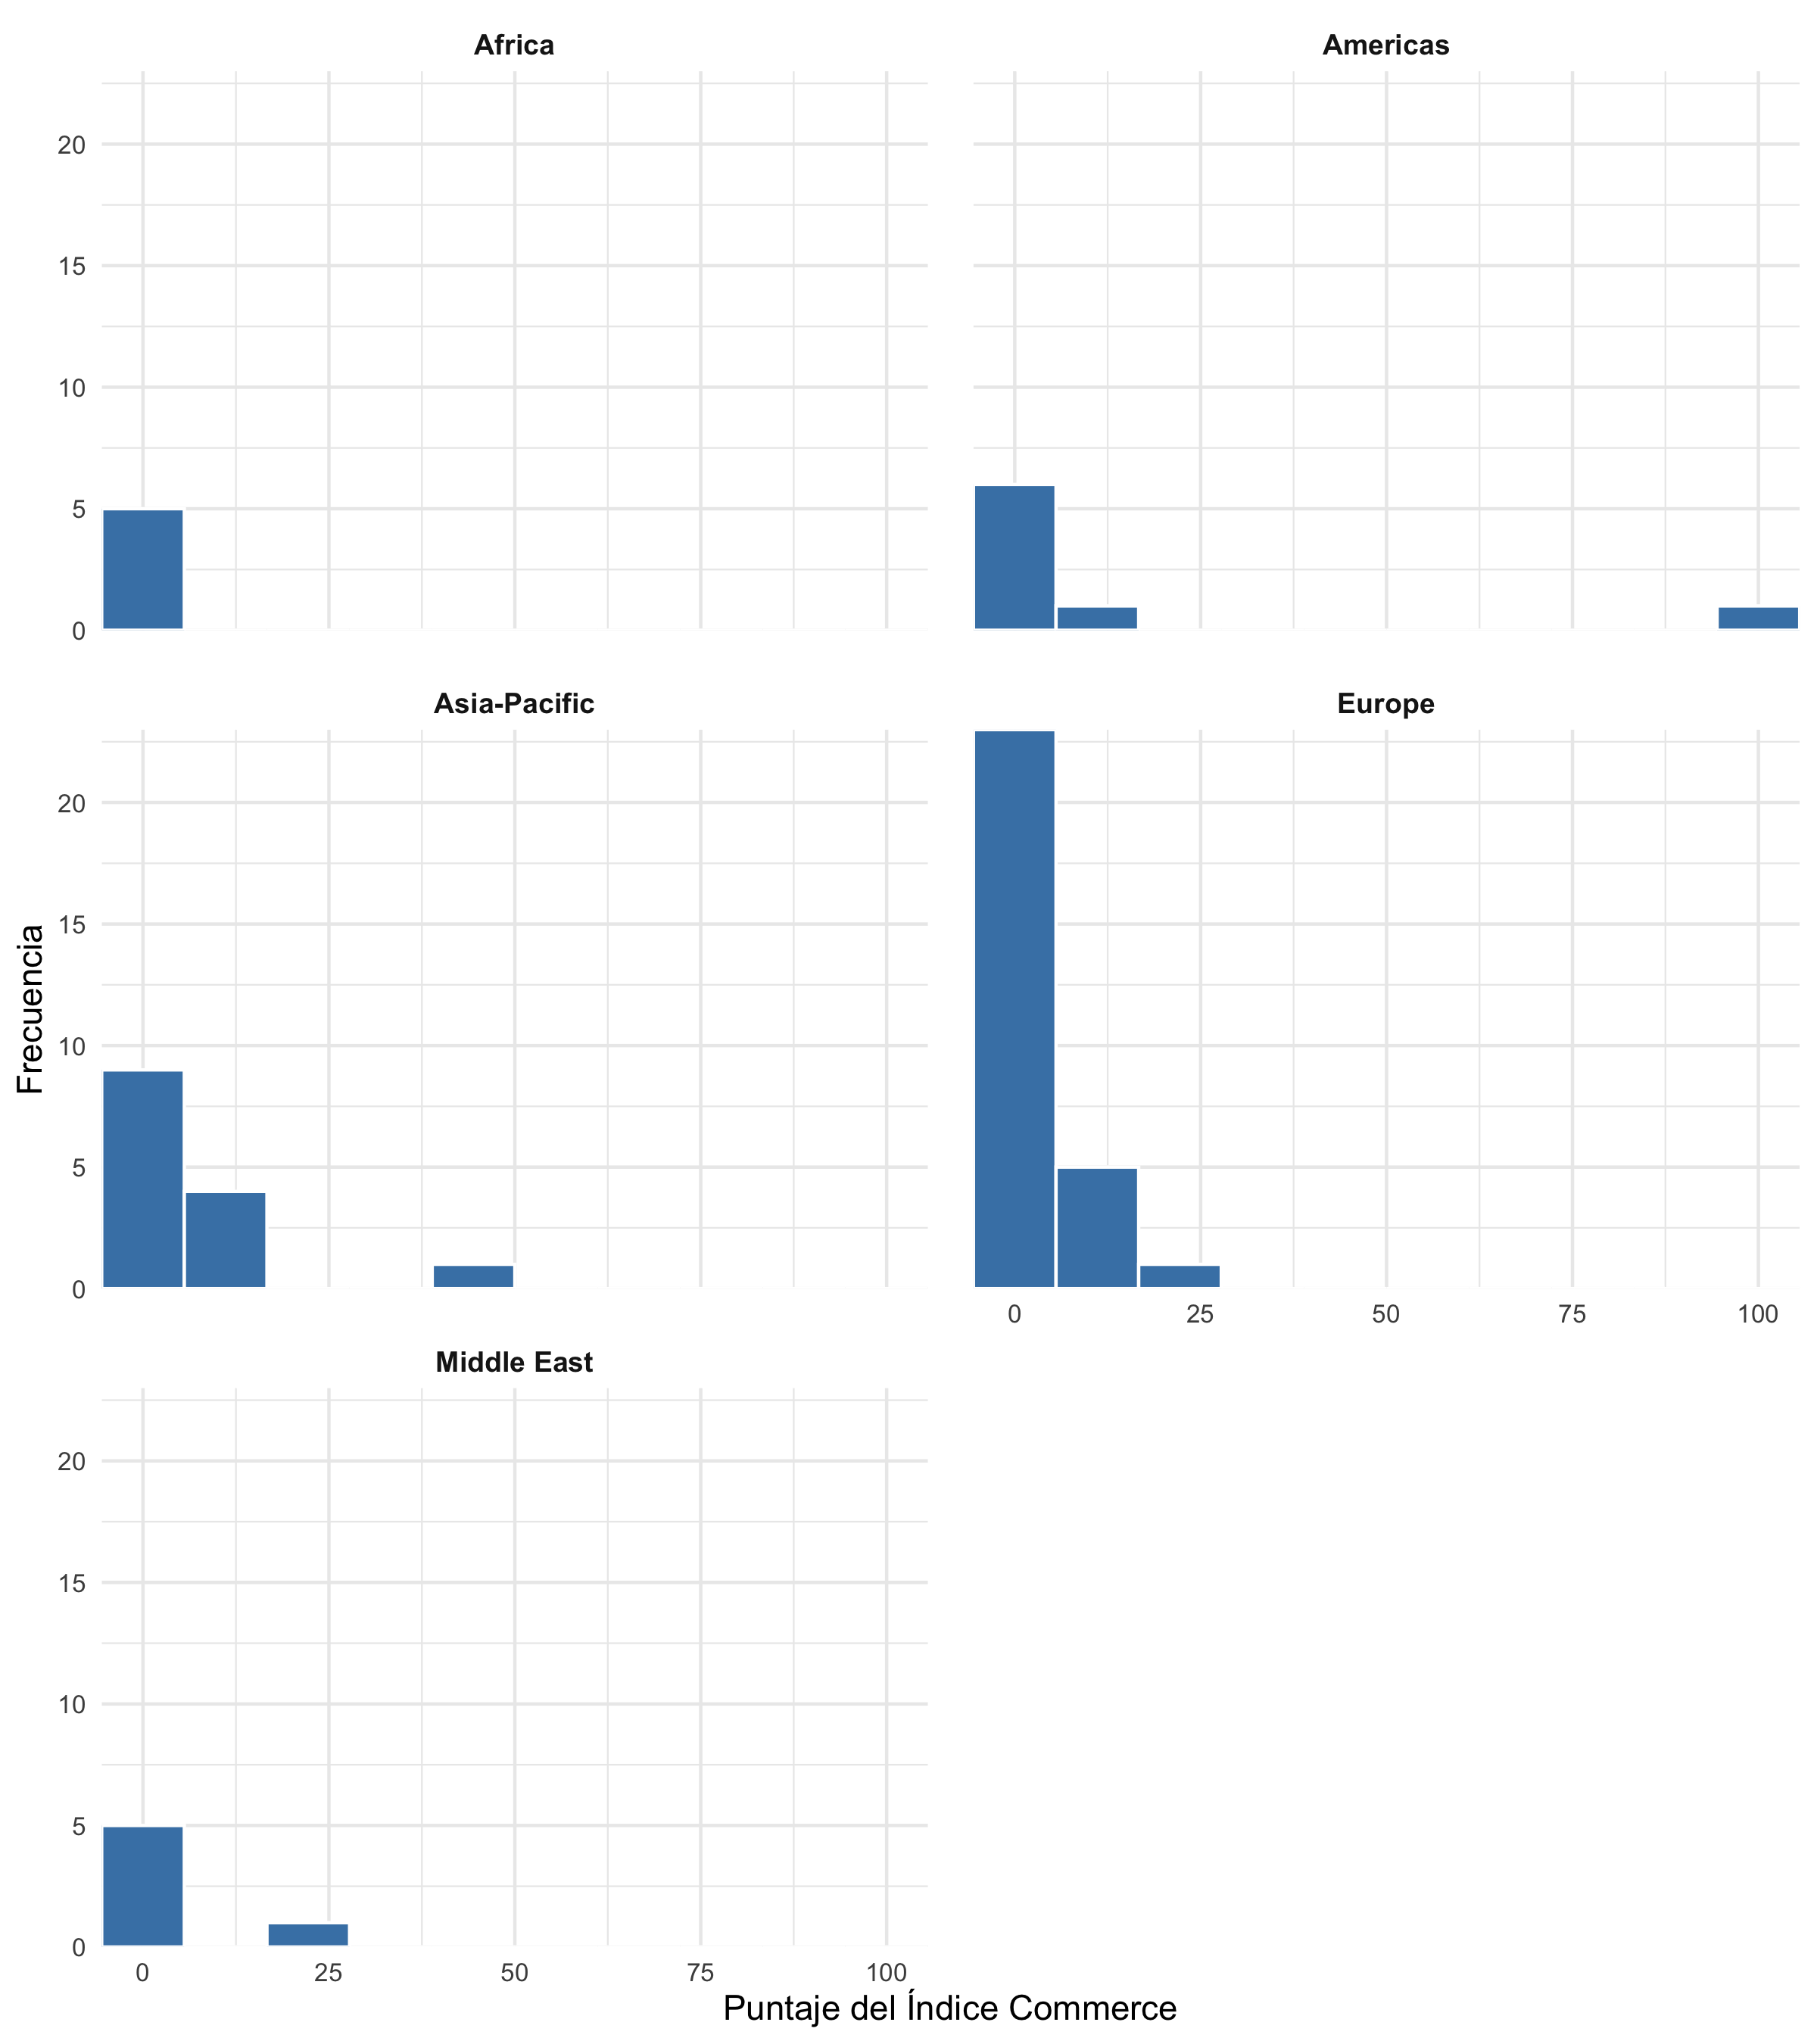
\includegraphics[width=\linewidth]{figura2.png}
\end{center}
Figura 2. Distribución del Índice Commerce agrupado por Región.


La Ojiva en la Figura 3 presenta la distriución acumulada de los datos de manera porcental, lo cuál permite estimar los percentiles correspondientes a los diferentes puntajes del índice Commerce.

En el caso de Americas, al rededor del 87.5\% de los datos tienen un índice Commmerce alrededor de 13 o menos, lo cuál indica una alta concentración de los datos a la izquierda del eje, sin embargo se presenta un salto abrupto en el índice que se distancia de los demás datos, indicando un posible dato atípico en el puntaje 100. Esto mismo ocurre en Middle East donde aproximadamente un 80\% de los datos tienen un puntaje de alrededor de 7 o menos y se presenta salto abrupto en el índice a un puntaje alrededor de 27.

Asia-Pacific y Europe presentan distribuciones similares, sin embargo en Europe los datos se ven más concentrados a la izquierda del eje. En ambos casos una mayoría cercana a 85\% de los datos tienen un índice de aproximadmente 20 o menos en Asia-Pacific y 10 o menos en Europe. Posteriormente a este punto se presenta un incremento gradual en los puntajes para los datos restantes.

En África cerca del 80\% de los datos están concentrados en un puntaje cercano a 0, lo cuál indica que posiblemente no hay simetría en la distribución por lo cuál esta no es normal.




\begin{center}
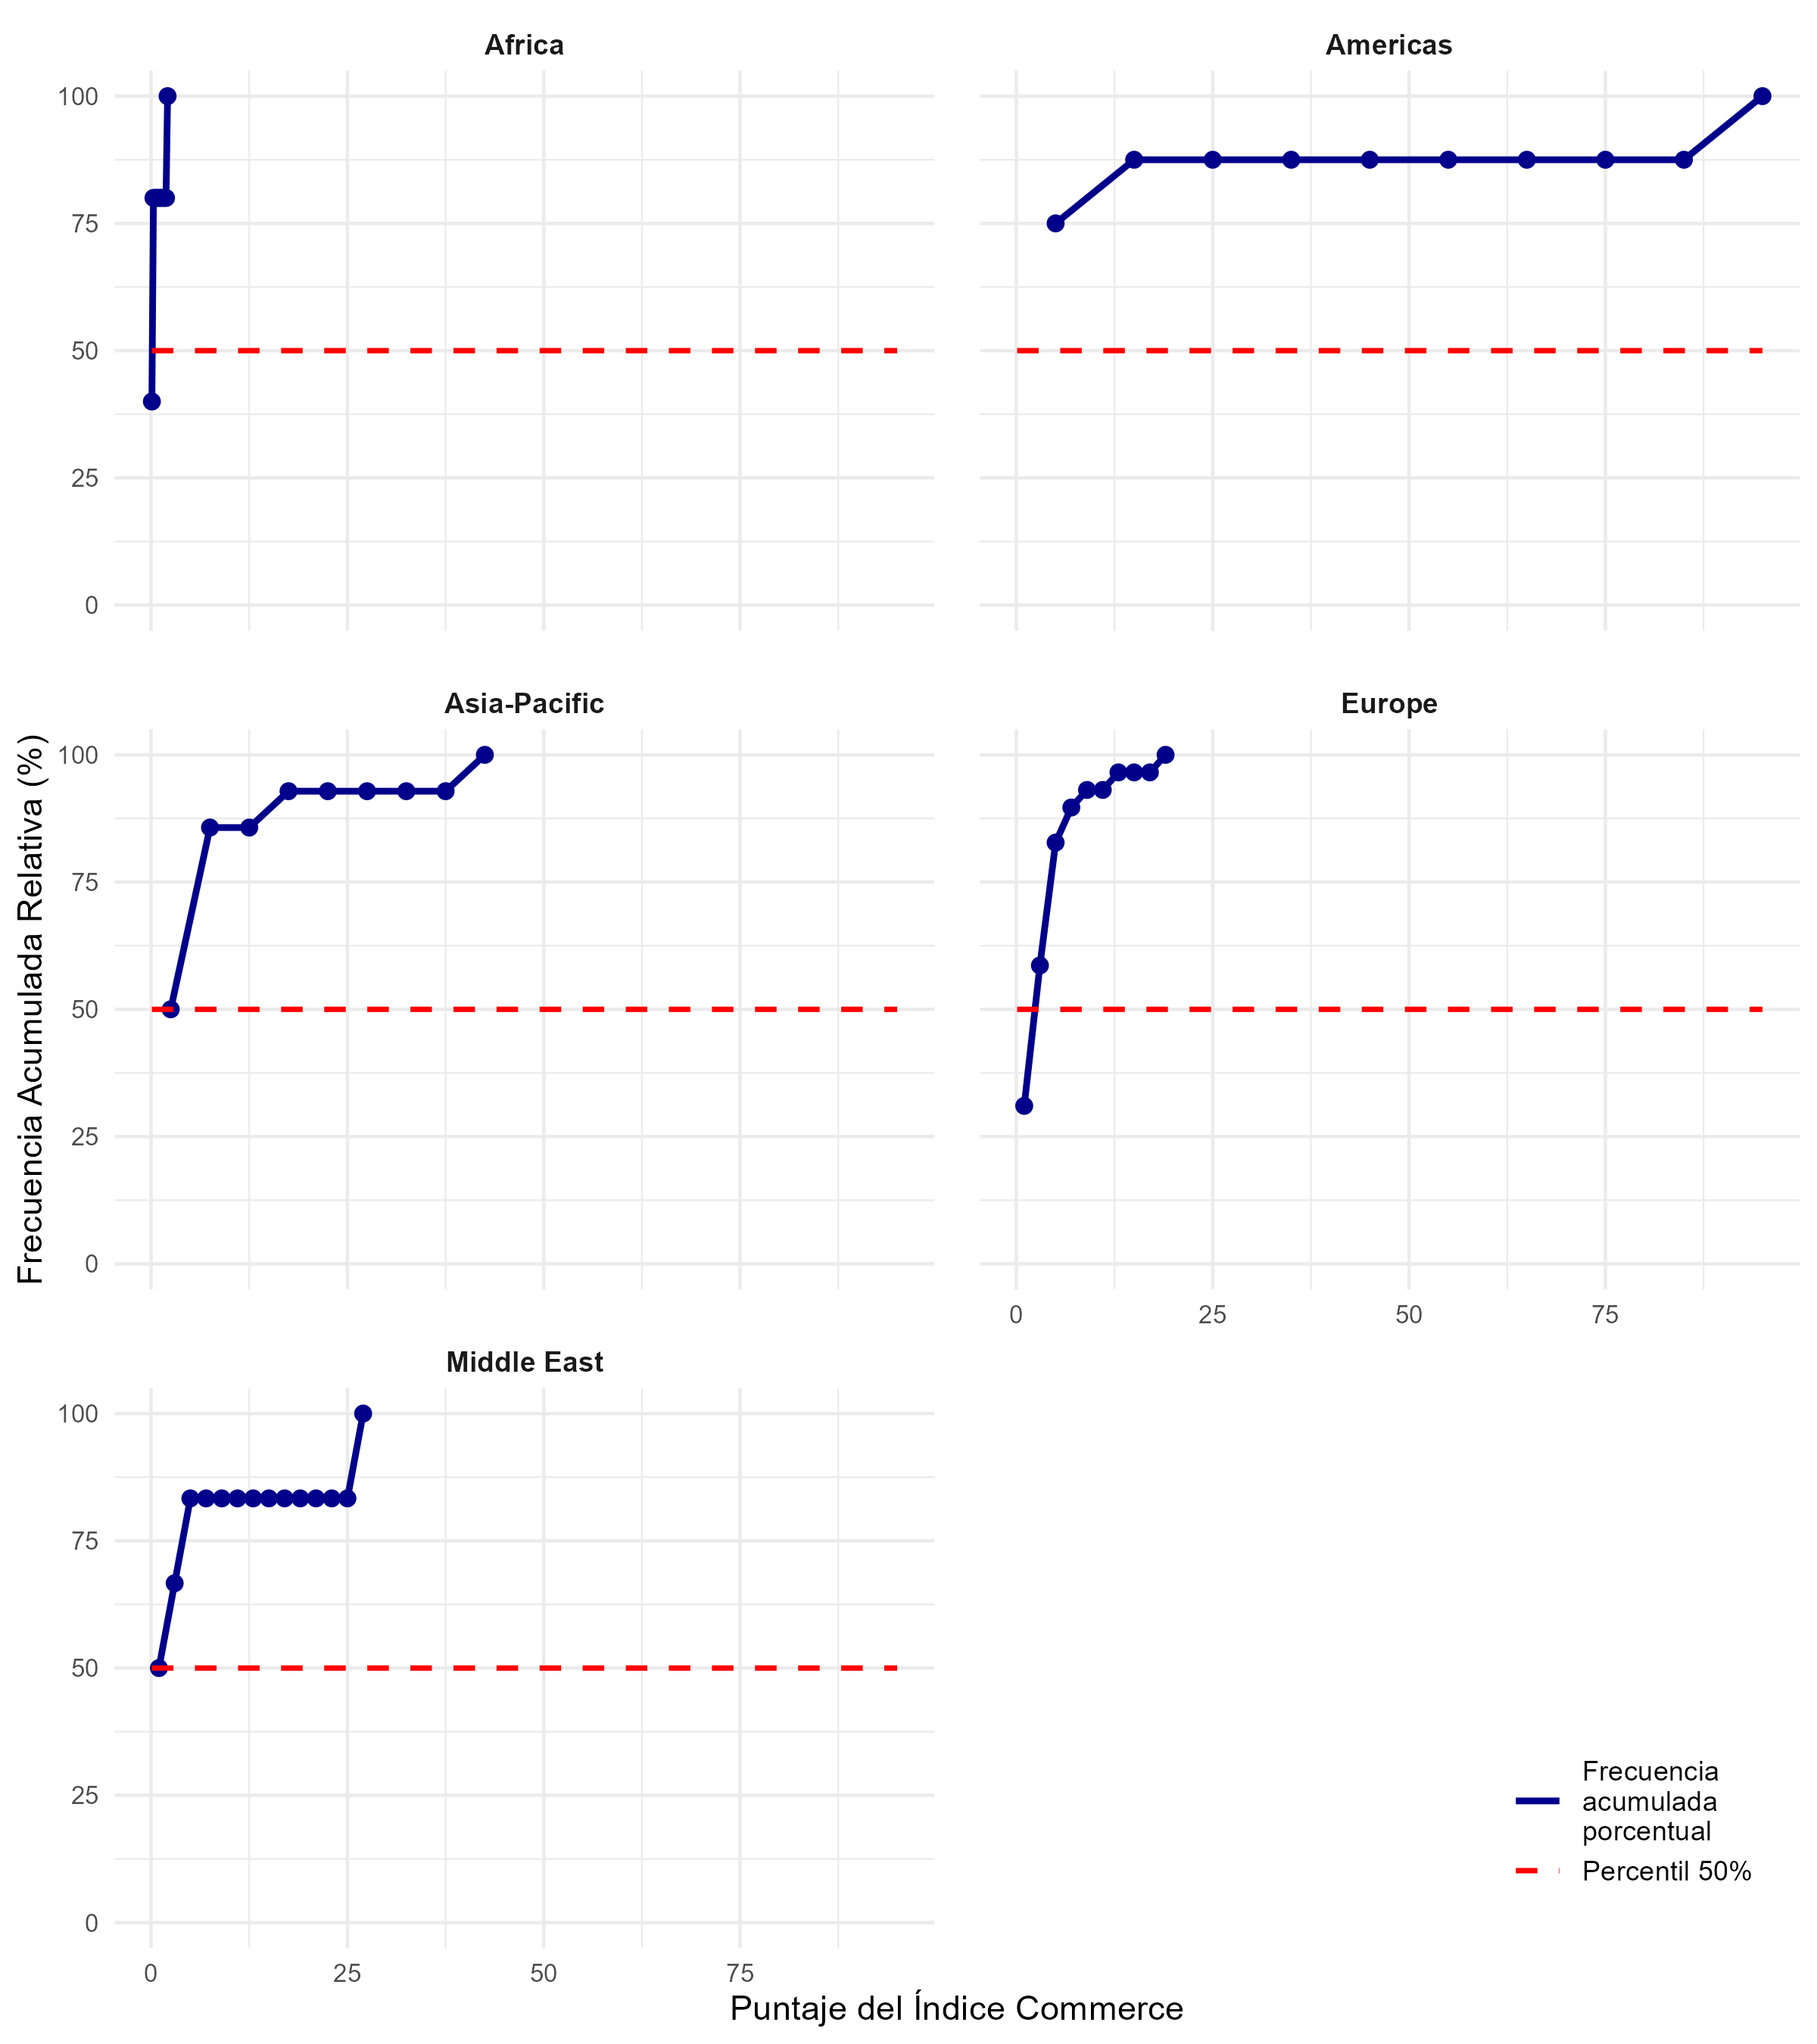
\includegraphics[width=\linewidth]{figura3.png}
\end{center}
Figura 3. Distribución acumulada del Índice Commerce agrupado por Región.


El diagrama de cajas y bigotes presentado en la Figura 4 presenta gráficamente las medidas de posición del Índice Commerce, la media e identifica los datos atípicos.

En el caso de Africa se muestra una muy alta compacidad de los datos donde la media es cercana a la mediana, cuartiles 1 y 3 y los límites inferiores y superiores de los bigotes. En este caso se presenta un dato atípico que se encuentra en relativa cercanía del límite superior del bigote.

En el caso de Americas se observa como el 50\% de los datos son altamente compactos, los datos entre la mediana y el Q3 tienen una disperción más alta y la media se aleja en gran medida (con un valor más alto que el límite superior del bigote) de la mediana debido a la presencia de 1 dato atípico a una gran distancia del resto de los datos al presentar un índice de 100. Esto también se observa en Asia-Pacific y Middle East, sin embargo en estos casos aunque hay un dato atípico que aleja la media del resto de los datos, la media se encuentra en un valor cercano al cuartil tres.

En el caso de Europe los datos se distribuyen de manera significativamente compacta. Aunque se presentan dos datos atípicos, la media se mantiene en relativa cercanía con la mediana.




\begin{center}
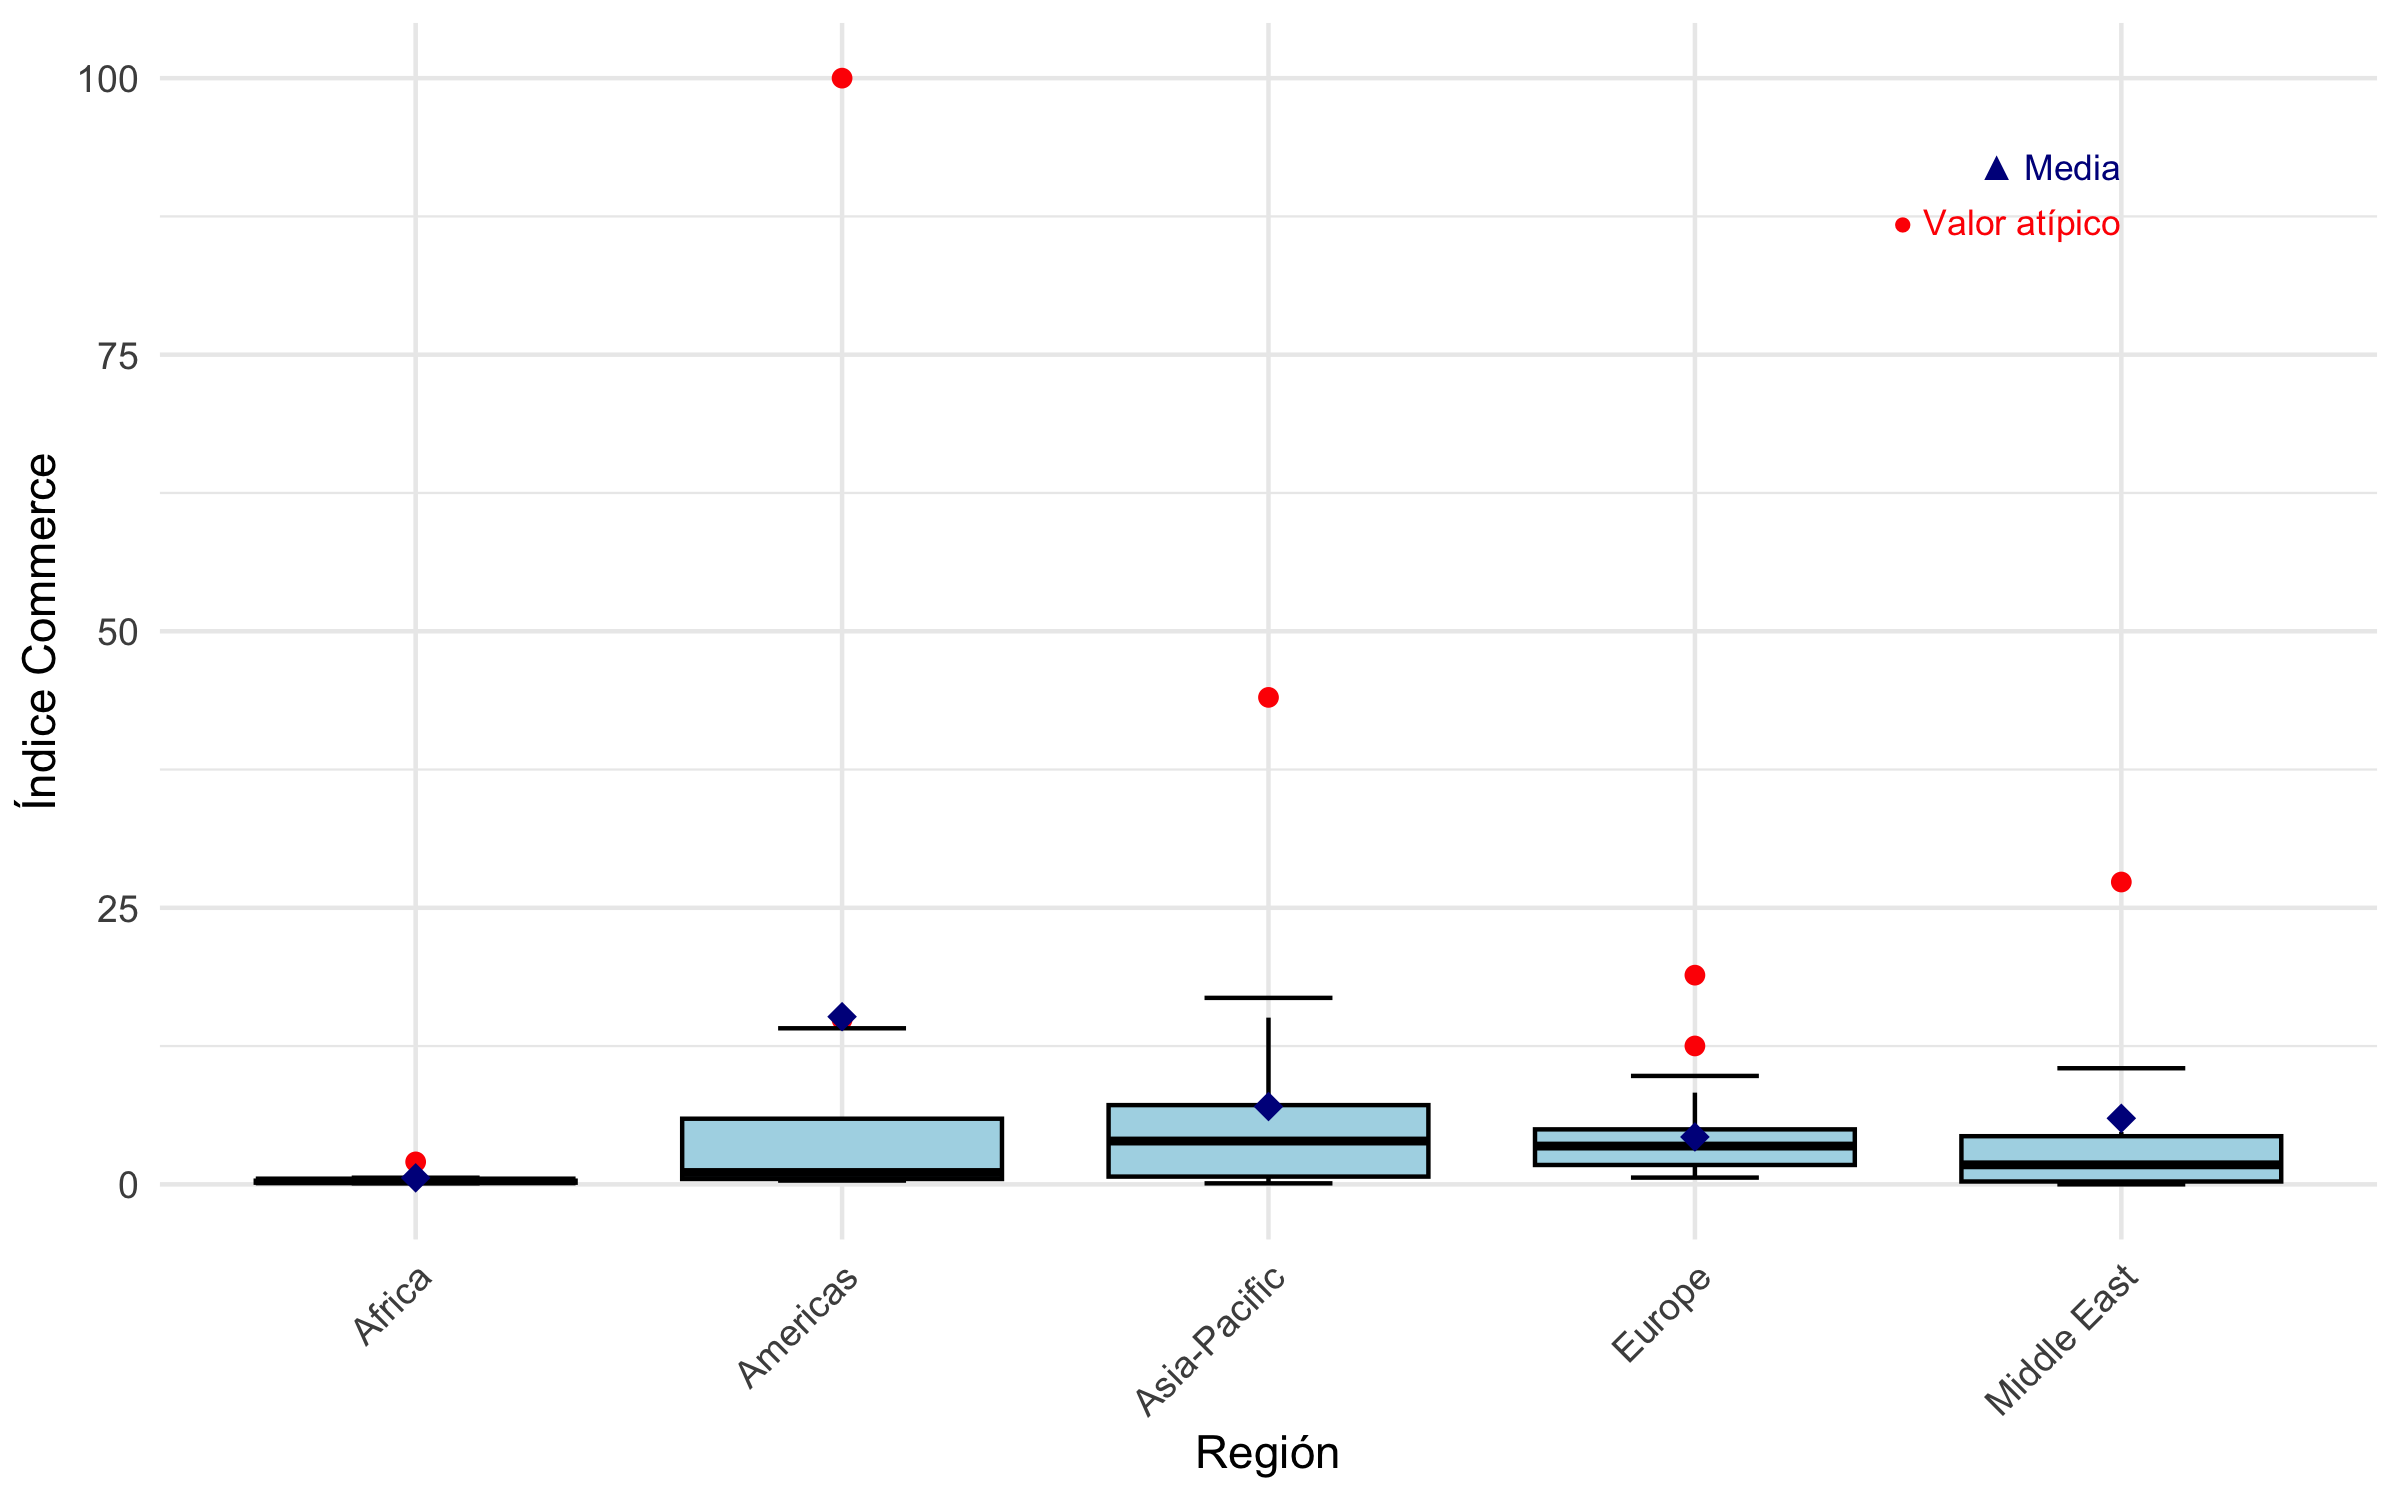
\includegraphics[width=\linewidth]{figura4.png}
\end{center}
Figura 4. Distribución cajas y bigoes del Índice Commerce agrupado por Región.


\subsection{Índice Research}

El indicador Research mide la producción científica y capacidad investigadora en inteligencia artificial, siendo un predictor clave del desarrollo tecnológico futuro. La Tabla 7 presenta su distribución global mediante frecuencias absolutas y relativas, permitiendo identificar los patrones de concentración del conocimiento especializado. Este análisis es fundamental para comprender qué países están liderando la generación de nuevo conocimiento en IA y qué regiones requieren fortalecer sus sistemas de investigación.

Los resultados revelan una concentración extrema en la capacidad investigadora: mientras el 60\% de los países se ubica por debajo de los 30 puntos (F.Rel.Acum = 0.60), solo un selecto grupo (15\%) supera los 70 puntos. Estados Unidos (100 puntos) y China (71.42) dominan claramente los intervalos superiores. Sin embargo, destaca que varios países europeos (Reino Unido 36.5, Alemania 35.84) mantienen capacidades significativas. La presencia casi nula de países africanos y latinoamericanos por encima de los 20 puntos (F.Abs = 2) evidencia un riesgo crítico de dependencia tecnológica.

\end{multicols}

\begin{longtable}[]{@{}lcccc@{}}
\caption{Frecuencia del Índice Research}\tabularnewline
\toprule\noalign{}
Intervalo & F.Absoluta & F.Relativa & F.Abs.Acum & F.Rel.Acum \\
\midrule\noalign{}
\endfirsthead
\toprule\noalign{}
Intervalo & F.Absoluta & F.Relativa & F.Abs.Acum & F.Rel.Acum \\
\midrule\noalign{}
\endhead
\bottomrule\noalign{}
\endlastfoot
{[}0,10{]} & 26 & 0.42 & 26 & 0.42 \\
(10,20{]} & 14 & 0.23 & 40 & 0.65 \\
(20,30{]} & 12 & 0.19 & 52 & 0.84 \\
(30,40{]} & 8 & 0.13 & 60 & 0.97 \\
(40,50{]} & 0 & 0.00 & 60 & 0.97 \\
(50,60{]} & 0 & 0.00 & 60 & 0.97 \\
(60,70{]} & 0 & 0.00 & 60 & 0.97 \\
(70,80{]} & 1 & 0.02 & 61 & 0.98 \\
(80,90{]} & 0 & 0.00 & 61 & 0.98 \\
(90,100{]} & 1 & 0.02 & 62 & 1.00 \\
\end{longtable}

\begin{multicols}{2}

La Tabla 8 presenta la distribución conjunta entre el Índice Research (A) y el Total Score (B), ambos agrupados en intervalos. A partir de los datos se puede observar que las frecuencias más altas se concentran en los rangos bajos de ambas variables. Por ejemplo, el intervalo [0,10] del Índice Research presenta un total de 26 observaciones, siendo el más frecuente, y dentro de este, los valores más altos se cruzan con [10,20] (14 observaciones) y [0,10] (9 observaciones) del Total Score.

En contraste, a medida que aumentan los valores tanto del Índice Research como del Total Score, las frecuencias disminuyen significativamente, llegando incluso a ser cero en varios cruces. Esto sugiere que la mayoría de los datos se concentran en valores bajos de ambas variables.

\end{multicols}

\renewcommand{\arraystretch}{1.3}
\begin{scriptsize}% latex table generated in R 4.4.2 by xtable 1.8-4 package
% Fri May 16 07:06:58 2025
\begin{longtable}{lrrrrrrrrrrr}
\caption{Tabla de Frecuencia Bivariada Índice Research (A) vs Total Score (B)} \\ 
  \hline
A   -   B & [0, 10] & (10, 20] & (20, 30] & (30, 40] & (40, 50] & (50, 60] & (60, 70] & (70, 80] & (80, 90] & (90, 100] & Total \\ 
  \hline
(0, 10] & 9.00 & 14.00 & 3.00 & 0.00 & 0.00 & 0.00 & 0.00 & 0.00 & 0.00 & 0.00 & 26.00 \\ 
  (10, 20] & 0.00 & 3.00 & 8.00 & 3.00 & 0.00 & 0.00 & 0.00 & 0.00 & 0.00 & 0.00 & 14.00 \\ 
  (20, 30] & 0.00 & 0.00 & 6.00 & 6.00 & 0.00 & 0.00 & 0.00 & 0.00 & 0.00 & 0.00 & 12.00 \\ 
  (30, 40] & 0.00 & 0.00 & 1.00 & 5.00 & 2.00 & 0.00 & 0.00 & 0.00 & 0.00 & 0.00 & 8.00 \\ 
  (40, 50] & 0.00 & 0.00 & 0.00 & 0.00 & 0.00 & 0.00 & 0.00 & 0.00 & 0.00 & 0.00 & 0.00 \\ 
  (50, 60] & 0.00 & 0.00 & 0.00 & 0.00 & 0.00 & 0.00 & 0.00 & 0.00 & 0.00 & 0.00 & 0.00 \\ 
  (60, 70] & 0.00 & 0.00 & 0.00 & 0.00 & 0.00 & 0.00 & 0.00 & 0.00 & 0.00 & 0.00 & 0.00 \\ 
  (70, 80] & 0.00 & 0.00 & 0.00 & 0.00 & 0.00 & 0.00 & 1.00 & 0.00 & 0.00 & 0.00 & 1.00 \\ 
  (80, 90] & 0.00 & 0.00 & 0.00 & 0.00 & 0.00 & 0.00 & 0.00 & 0.00 & 0.00 & 0.00 & 0.00 \\ 
  (90, 100] & 0.00 & 0.00 & 0.00 & 0.00 & 0.00 & 0.00 & 0.00 & 0.00 & 0.00 & 1.00 & 1.00 \\ 
  Total & 9.00 & 17.00 & 18.00 & 14.00 & 2.00 & 0.00 & 1.00 & 0.00 & 0.00 & 1.00 & 62.00 \\ 
   \hline
\hline
\end{longtable}
\end{scriptsize}\renewcommand{\arraystretch}{1}

\begin{multicols}{2}

La Figura 5 muestra la distribución del Índice Research en distintas regiones del mundo. Se observa que la mayoría de las regiones, como África, Medio Oriente y América, presentan una fuerte concentración de países con puntajes bajos, lo que indica un nivel limitado de desarrollo en investigación. En cambio, Europa y Asia-Pacífico muestran distribuciones más variadas, con una mayor presencia de países en niveles intermedios e incluso altos, lo cual sugiere un mejor desempeño en términos de inversión y producción científica. También se destacan algunos casos atípicos en regiones como América y Asia-Pacífico, que muestran países con puntajes significativamente superiores al resto.



\begin{center}
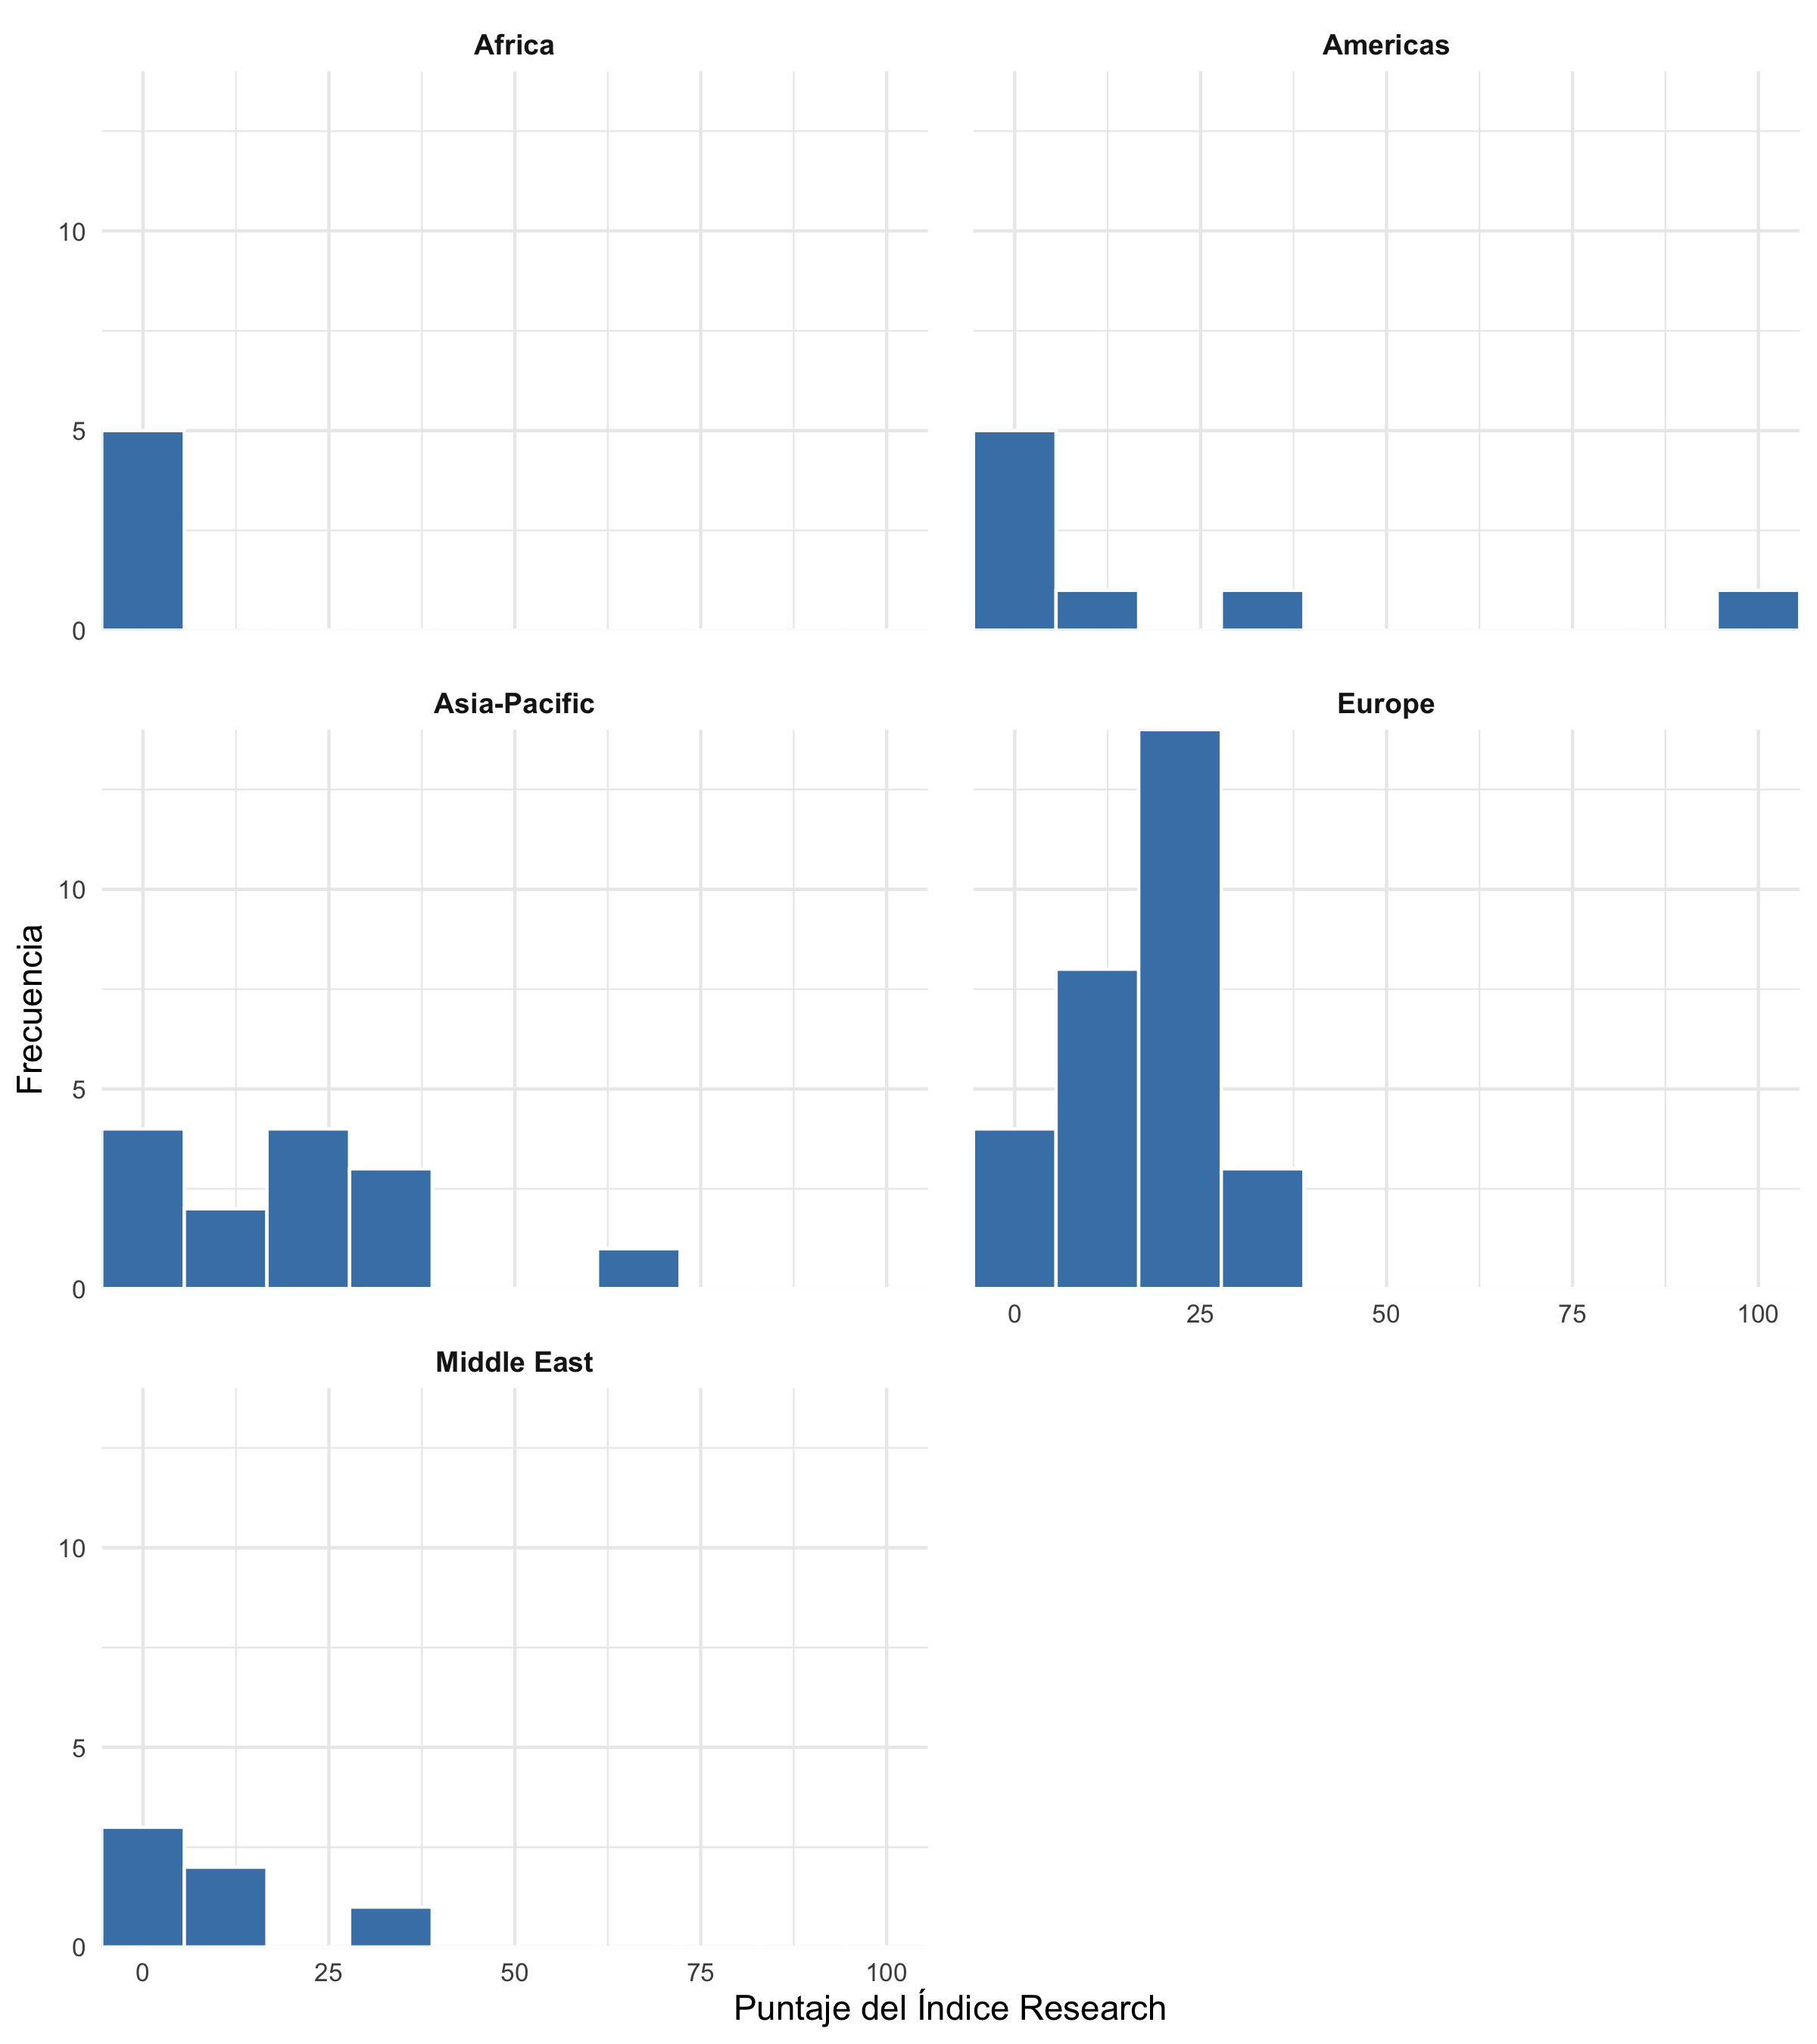
\includegraphics[width=\linewidth]{figura5.png}
\end{center}
Figura 5. Distribución del Índice Research agrupado por Región.

En la Figura 6 Africa presenta una distribución muy concentrada en valores bajos (menores a 5), lo cual indica poca variabilidad y bajo desempeño general en el índice. Americas, aunque hay un poco más de dispersión en comparación con África, la mayoría de los países también se concentran en valores menores a 30, con pocos casos en niveles altos. Asia-Pacific tiene una distribución más balanceada, con varios países en rangos intermedios y algunos casos en valores altos del índice. Supera el percentil 50 antes que otras regiones.Europe muestra una tendencia progresiva con valores mejor distribuidos. Muchos países alcanzan o superan el percentil 50, lo que indica un mejor desempeño relativo y Middle East: Tiene una distribución similar a África, con acumulaciones rápidas en valores bajos y pocos países con puntajes elevados.

En general, se observa que Europa y Asia-Pacífico presentan un comportamiento más diverso y favorable en el Índice Research, mientras que regiones como África y Medio Oriente concentran sus frecuencias en los niveles más bajos.




\begin{center}
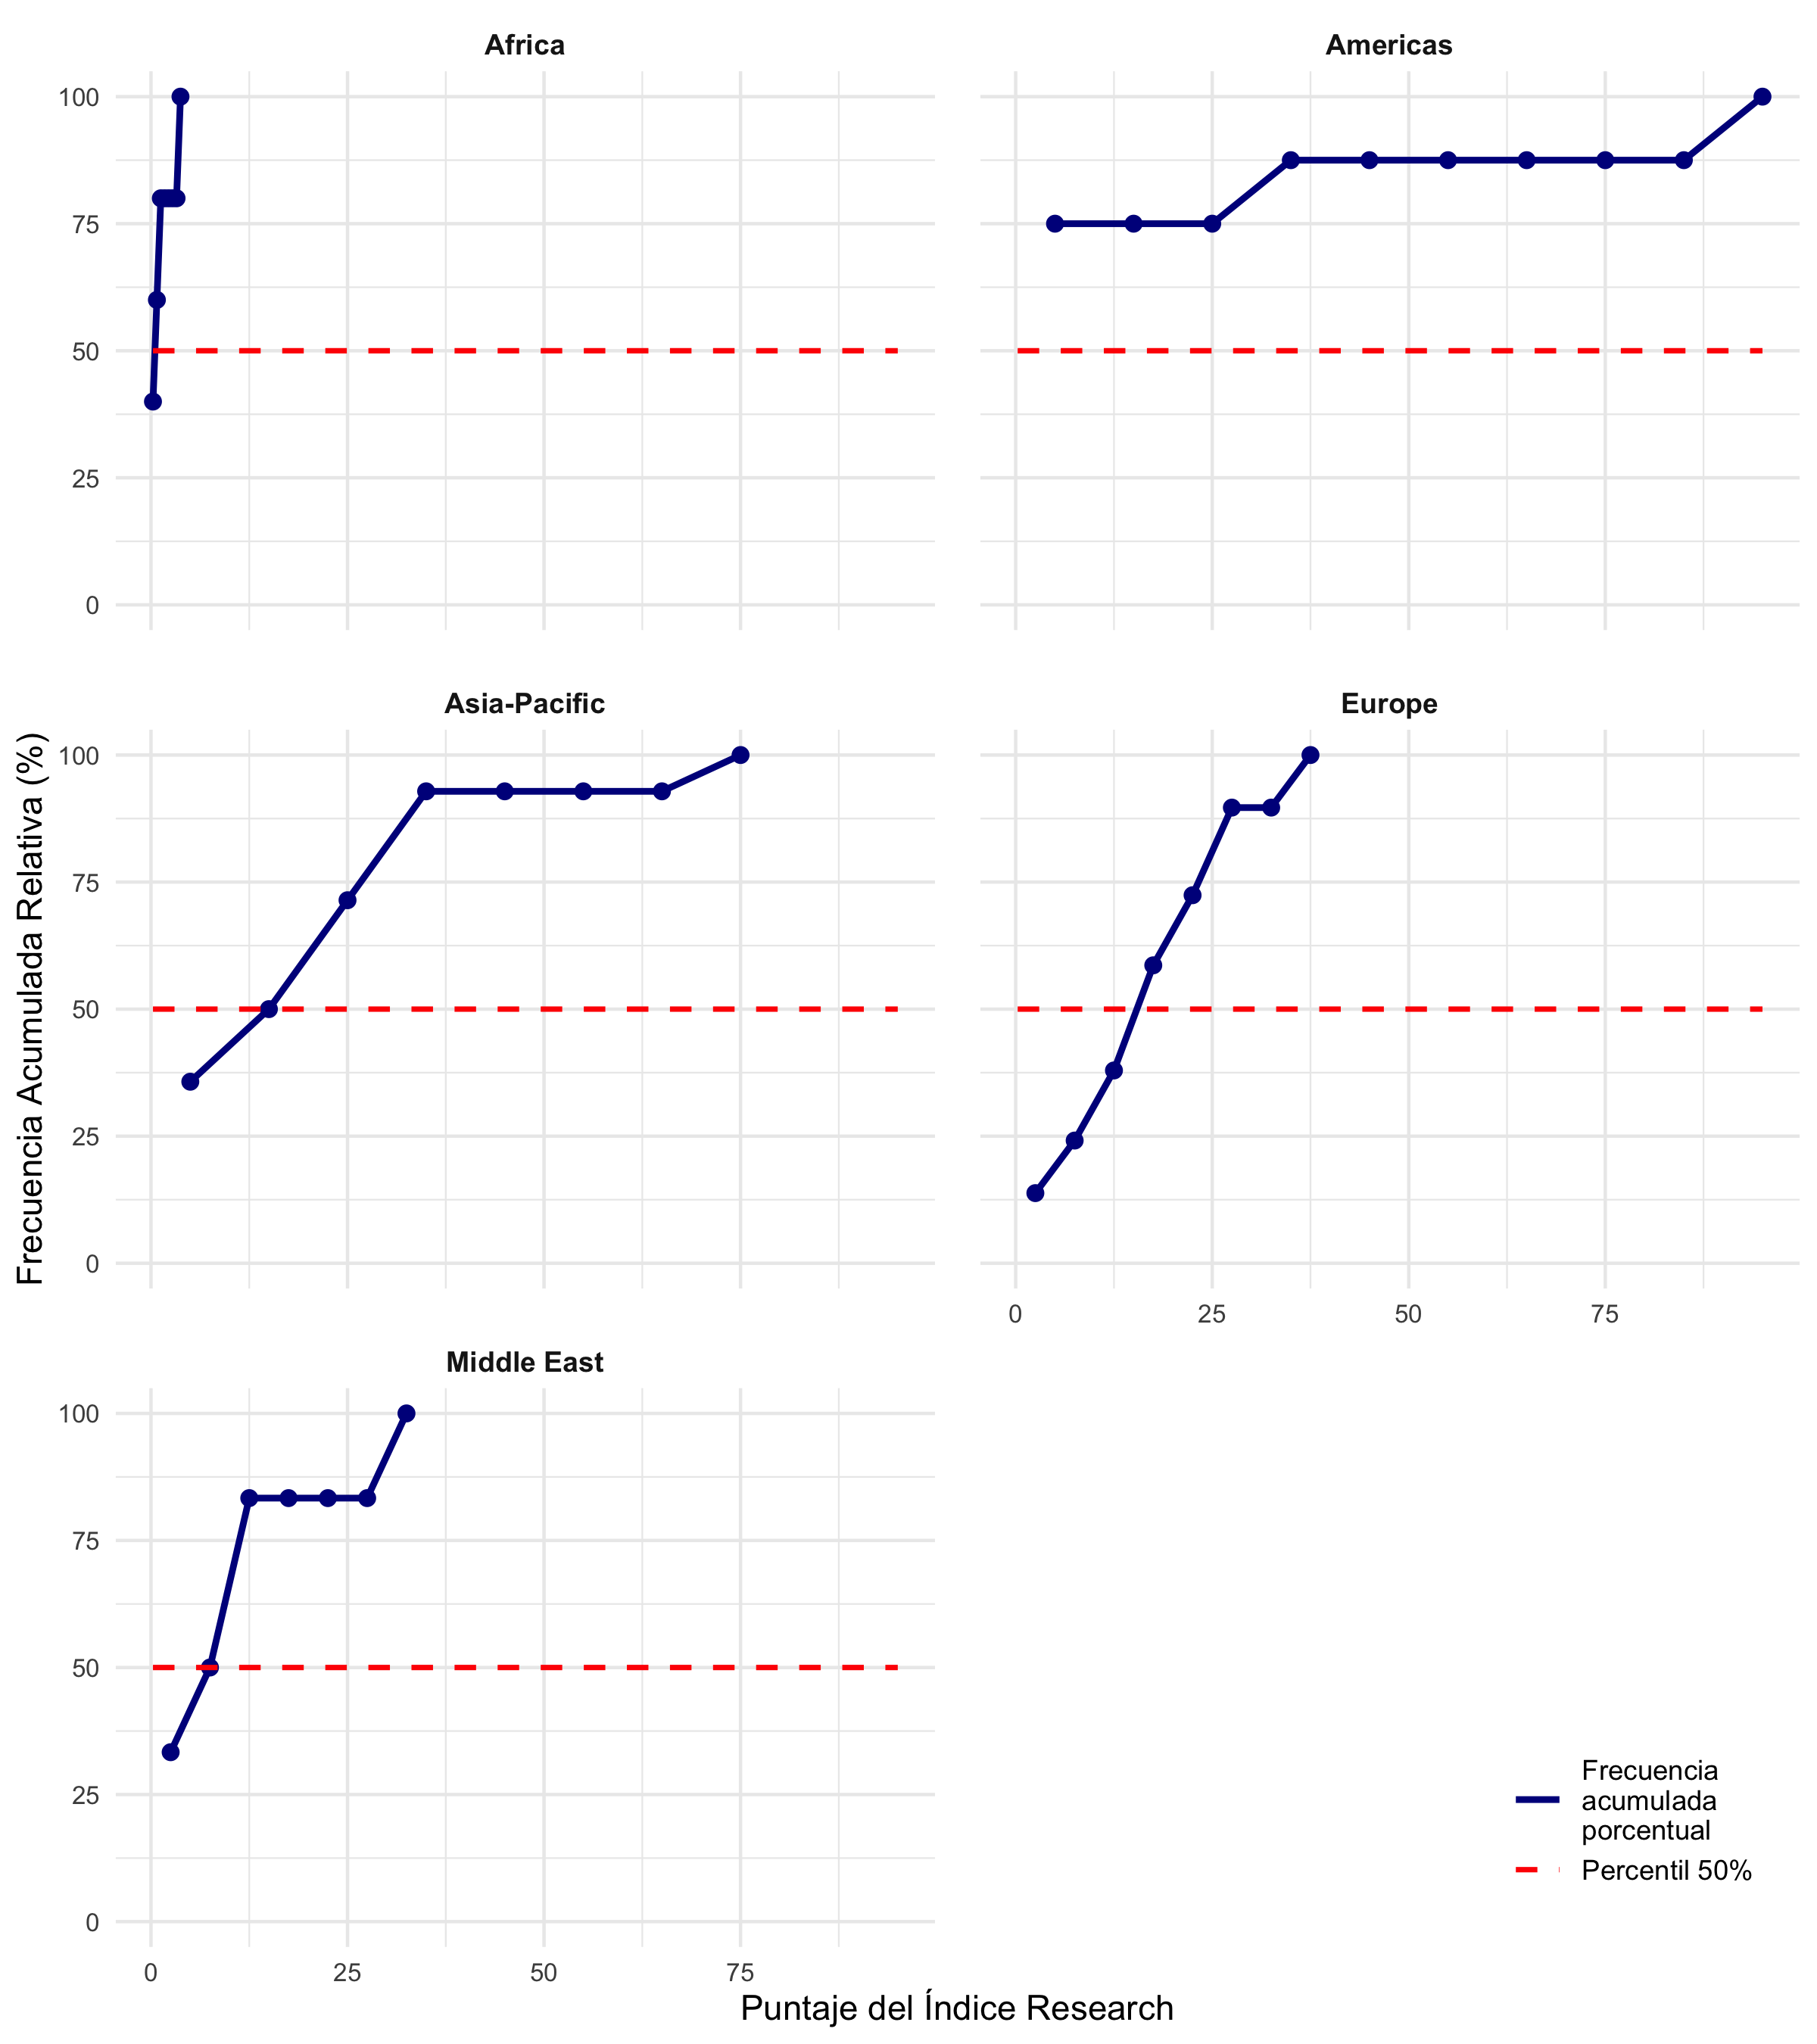
\includegraphics[width=\linewidth]{figura6.png}
\end{center}
Figura 6. Distribución acumulada del Índice Research agrupado por Región.

La Figura 7 compara las regiones usando diagramas de caja, que nos permiten ver cómo se distribuyen los datos, la mediana, y si hay valores atípicos (puntos rojos).

África tiene una caja muy pequeña y pegada al valor mínimo. Eso muestra que los datos están muy concentrados en valores bajos y no hay mucha variación. En América, la mediana sigue siendo baja, pero la caja es un poco más grande. Además, hay un valor atípico bastante alto, lo que significa que hay al menos un país con un nivel de investigación mucho mayor al resto. Asia-Pacífico es la región con mayor dispersión. Su mediana es más alta y tiene varios valores extremos, lo cual indica que hay países con niveles muy diferentes entre sí.Europa muestra una distribución más equilibrada, con una mediana relativamente alta y sin valores atípicos tan extremos. Esto sugiere que la mayoría de sus países tienen un desempeño aceptable en investigación y Medio Oriente tiene una mediana baja y poca dispersión, aunque también se observa un valor atípico.

En general, se nota que Europa y Asia-Pacífico destacan por tener mejores y más variados puntajes, mientras que África y Medio Oriente tienden a concentrarse en la parte baja del índice.



\begin{center}
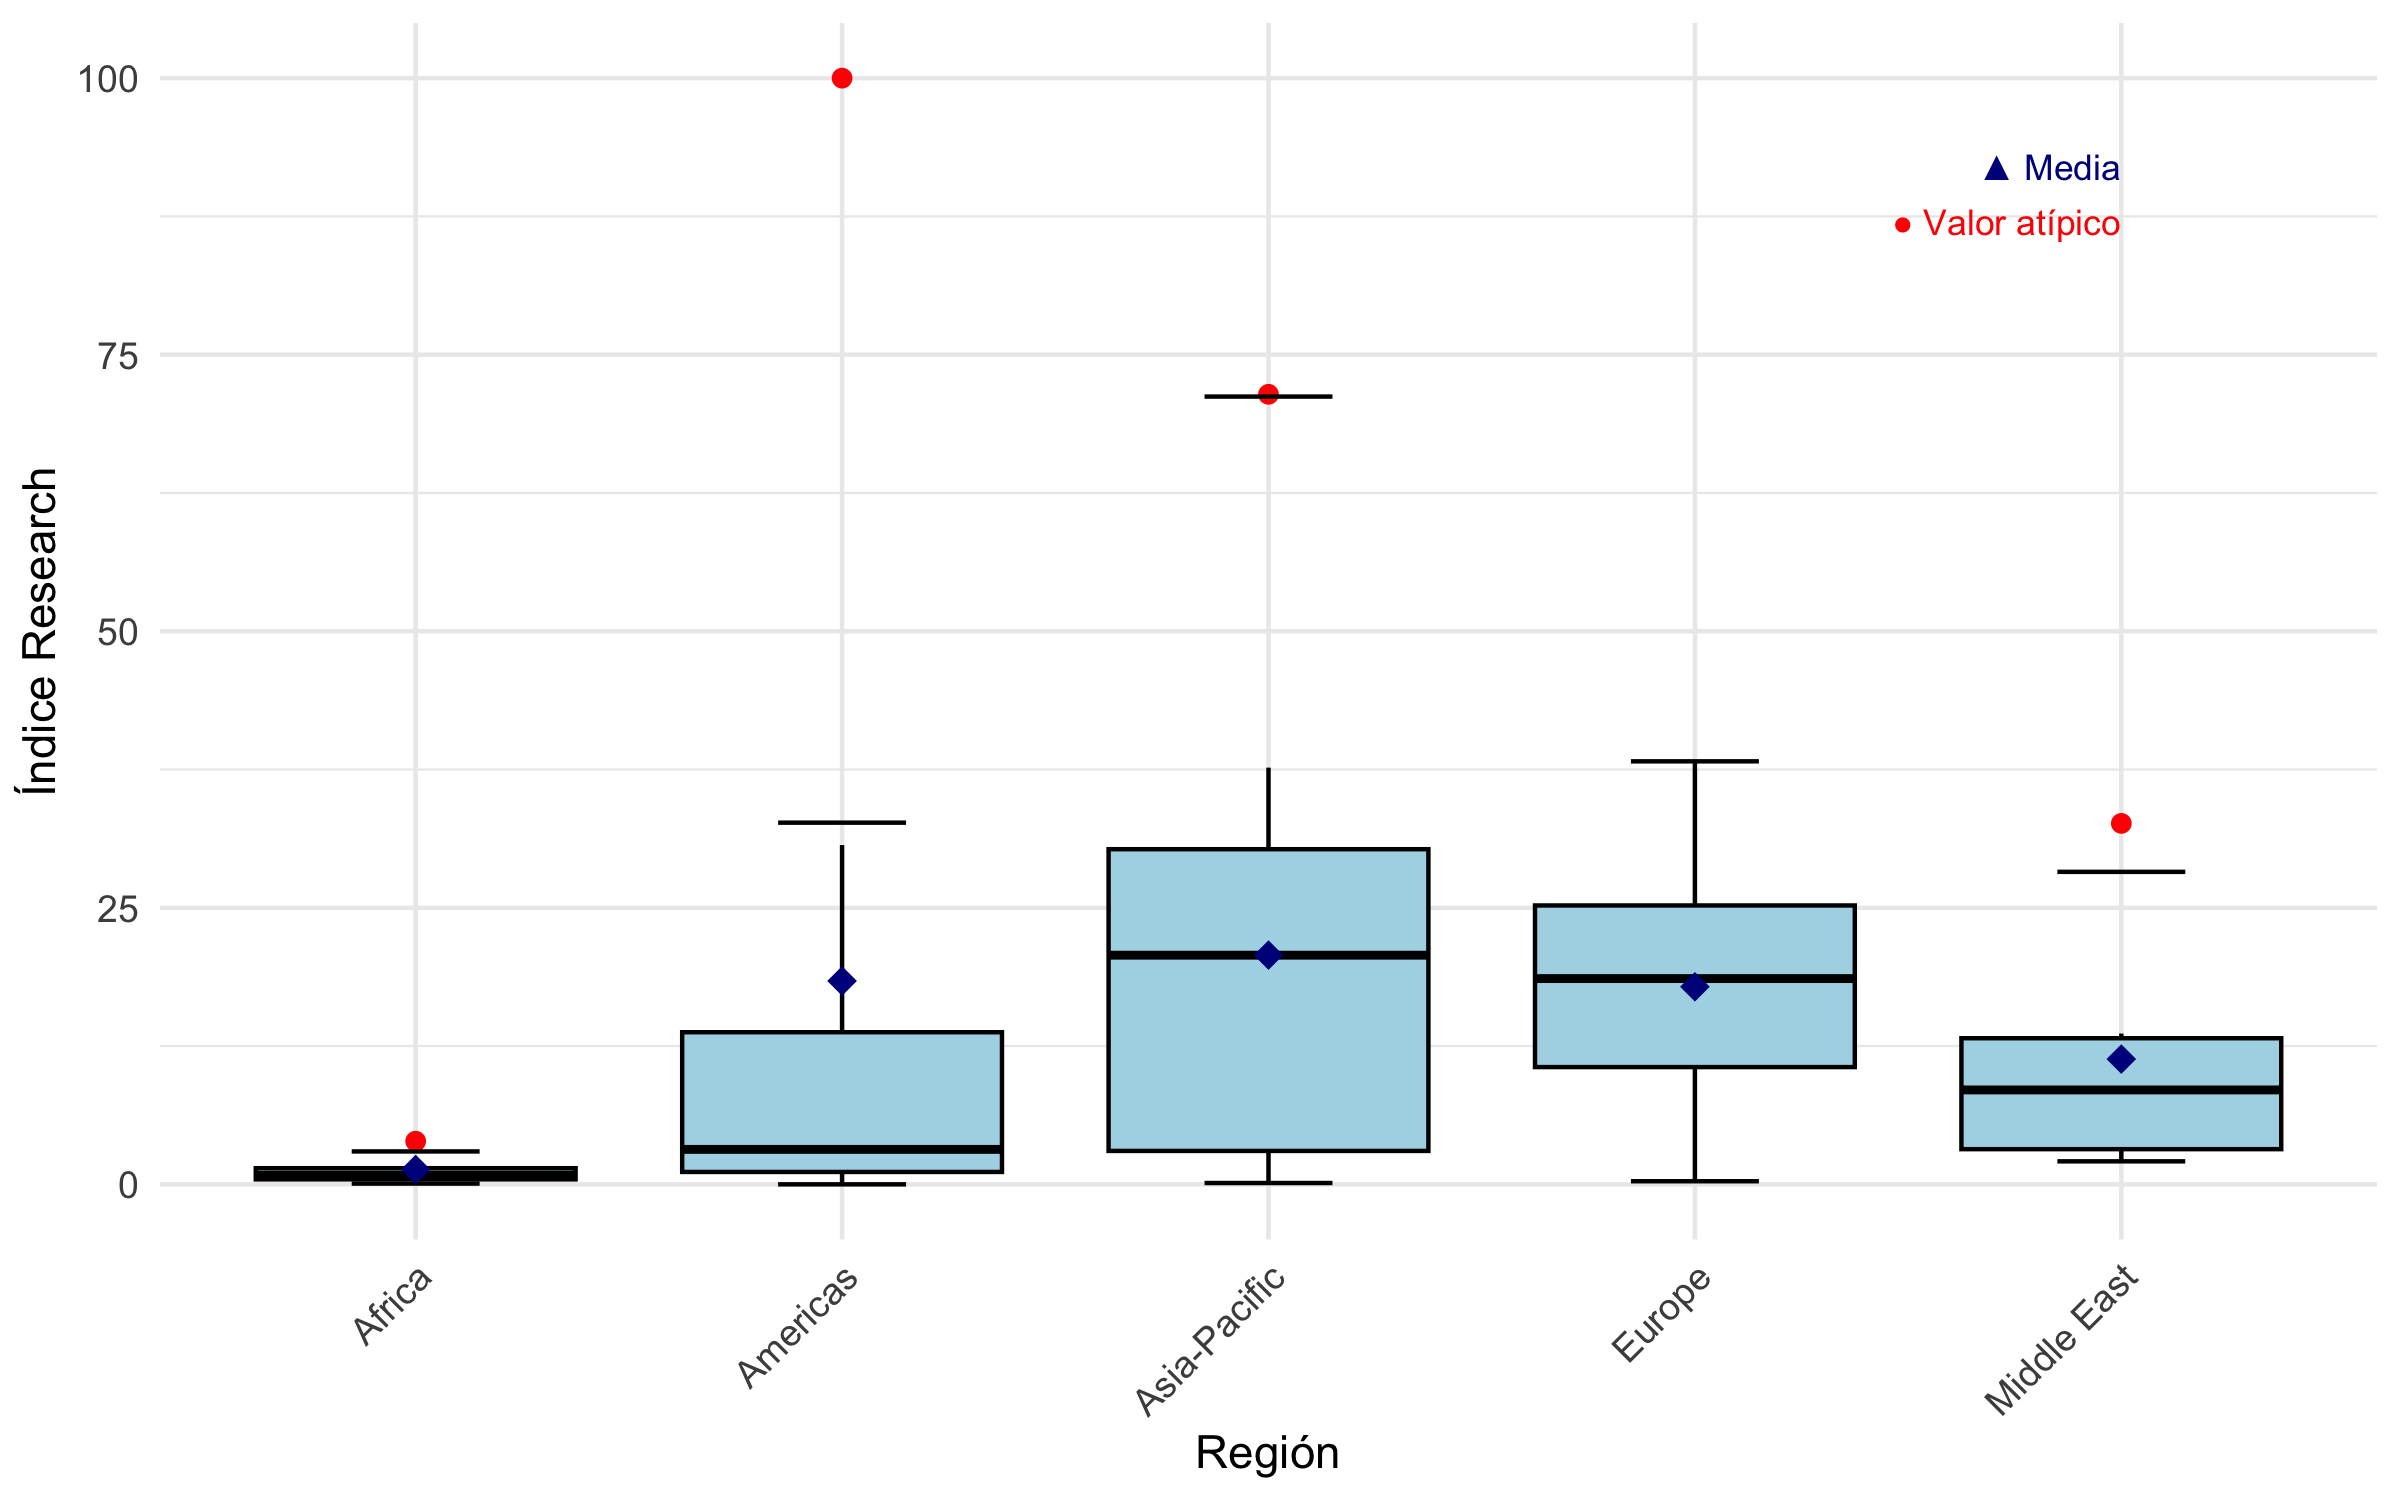
\includegraphics[width=\linewidth]{figura7.png}
\end{center}
Figura 7. Distribución cajas y bigotes del Índice Research agrupado por Región.


\subsection{Índice Talent}

La Tabla 9 revela una distribución desigual del talento en IA a nivel mundial, con una marcada concentración en los extremos: mientras el 42\% de los países se ubica en el rango más bajo (0-20 puntos), solo un 18 pot ciento supera los 50 puntos. Las frecuencias acumuladas muestran que apenas el 30 por ciento de las naciones alcanza niveles competitivos (mayor igual a 40 puntos), destacando Estados Unidos (100 puntos) como caso excepcional. Esta polarización refleja brechas estructurales en la formación de profesionales calificados, donde economías desarrolladas capturan la mayor parte del talento global.

La Tabla 8 revela una fuerte desigualdad en la distribución global de talento en IA. Estados Unidos destaca como líder absoluto (100 puntos), mientras que más del 40 por ciento de los países se concentra en el nivel más bajo (0-20 puntos). Esta brecha refleja las profundas asimetrías en desarrollo tecnológico, donde solo un puñado de naciones concentra las capacidades avanzadas.

La escasez de países en rangos intermedios (30-60 puntos) es particularmente preocupante, pues muestra que pocas economías están logrando desarrollar talento competitivo. Estos resultados subrayan la urgencia de políticas globales para democratizar el acceso a formación especializada, especialmente en regiones en desarrollo donde el talento en IA resulta crítico para no quedar rezagados en la transformación digital.

\end{multicols}

\begin{longtable}[]{@{}lcccc@{}}
\caption{Frecuencia del Índice Talent}\tabularnewline
\toprule\noalign{}
Intervalo & F.Absoluta & F.Relativa & F.Abs.Acum & F.Rel.Acum \\
\midrule\noalign{}
\endfirsthead
\toprule\noalign{}
Intervalo & F.Absoluta & F.Relativa & F.Abs.Acum & F.Rel.Acum \\
\midrule\noalign{}
\endhead
\bottomrule\noalign{}
\endlastfoot
{[}0,10{]} & 22 & 0.35 & 22 & 0.35 \\
(10,20{]} & 22 & 0.35 & 44 & 0.71 \\
(20,30{]} & 11 & 0.18 & 55 & 0.89 \\
(30,40{]} & 5 & 0.08 & 60 & 0.97 \\
(40,50{]} & 1 & 0.02 & 61 & 0.98 \\
(50,60{]} & 0 & 0.00 & 61 & 0.98 \\
(60,70{]} & 0 & 0.00 & 61 & 0.98 \\
(70,80{]} & 0 & 0.00 & 61 & 0.98 \\
(80,90{]} & 0 & 0.00 & 61 & 0.98 \\
(90,100{]} & 1 & 0.02 & 62 & 1.00 \\
\end{longtable}

\textbackslash{}

\renewcommand{\arraystretch}{1.3}
\begin{scriptsize}% latex table generated in R 4.4.2 by xtable 1.8-4 package
% Fri May 16 07:06:58 2025
\begin{longtable}{lrrrrrrrrrrr}
\caption{Tabla de Frecuencia Bivariada Índice Talent (A) vs Total Score (B)} \\ 
  \hline
A   -   B & [0, 10] & (10, 20] & (20, 30] & (30, 40] & (40, 50] & (50, 60] & (60, 70] & (70, 80] & (80, 90] & (90, 100] & Total \\ 
  \hline
(0, 10] & 9.00 & 11.00 & 2.00 & 0.00 & 0.00 & 0.00 & 0.00 & 0.00 & 0.00 & 0.00 & 22.00 \\ 
  (10, 20] & 0.00 & 6.00 & 13.00 & 2.00 & 0.00 & 0.00 & 1.00 & 0.00 & 0.00 & 0.00 & 22.00 \\ 
  (20, 30] & 0.00 & 0.00 & 3.00 & 8.00 & 0.00 & 0.00 & 0.00 & 0.00 & 0.00 & 0.00 & 11.00 \\ 
  (30, 40] & 0.00 & 0.00 & 0.00 & 3.00 & 2.00 & 0.00 & 0.00 & 0.00 & 0.00 & 0.00 & 5.00 \\ 
  (40, 50] & 0.00 & 0.00 & 0.00 & 1.00 & 0.00 & 0.00 & 0.00 & 0.00 & 0.00 & 0.00 & 1.00 \\ 
  (50, 60] & 0.00 & 0.00 & 0.00 & 0.00 & 0.00 & 0.00 & 0.00 & 0.00 & 0.00 & 0.00 & 0.00 \\ 
  (60, 70] & 0.00 & 0.00 & 0.00 & 0.00 & 0.00 & 0.00 & 0.00 & 0.00 & 0.00 & 0.00 & 0.00 \\ 
  (70, 80] & 0.00 & 0.00 & 0.00 & 0.00 & 0.00 & 0.00 & 0.00 & 0.00 & 0.00 & 0.00 & 0.00 \\ 
  (80, 90] & 0.00 & 0.00 & 0.00 & 0.00 & 0.00 & 0.00 & 0.00 & 0.00 & 0.00 & 0.00 & 0.00 \\ 
  (90, 100] & 0.00 & 0.00 & 0.00 & 0.00 & 0.00 & 0.00 & 0.00 & 0.00 & 0.00 & 1.00 & 1.00 \\ 
  Total & 9.00 & 17.00 & 18.00 & 14.00 & 2.00 & 0.00 & 1.00 & 0.00 & 0.00 & 1.00 & 62.00 \\ 
   \hline
\hline
\end{longtable}
\end{scriptsize}\renewcommand{\arraystretch}{1}

\begin{multicols}{2}




\begin{center}
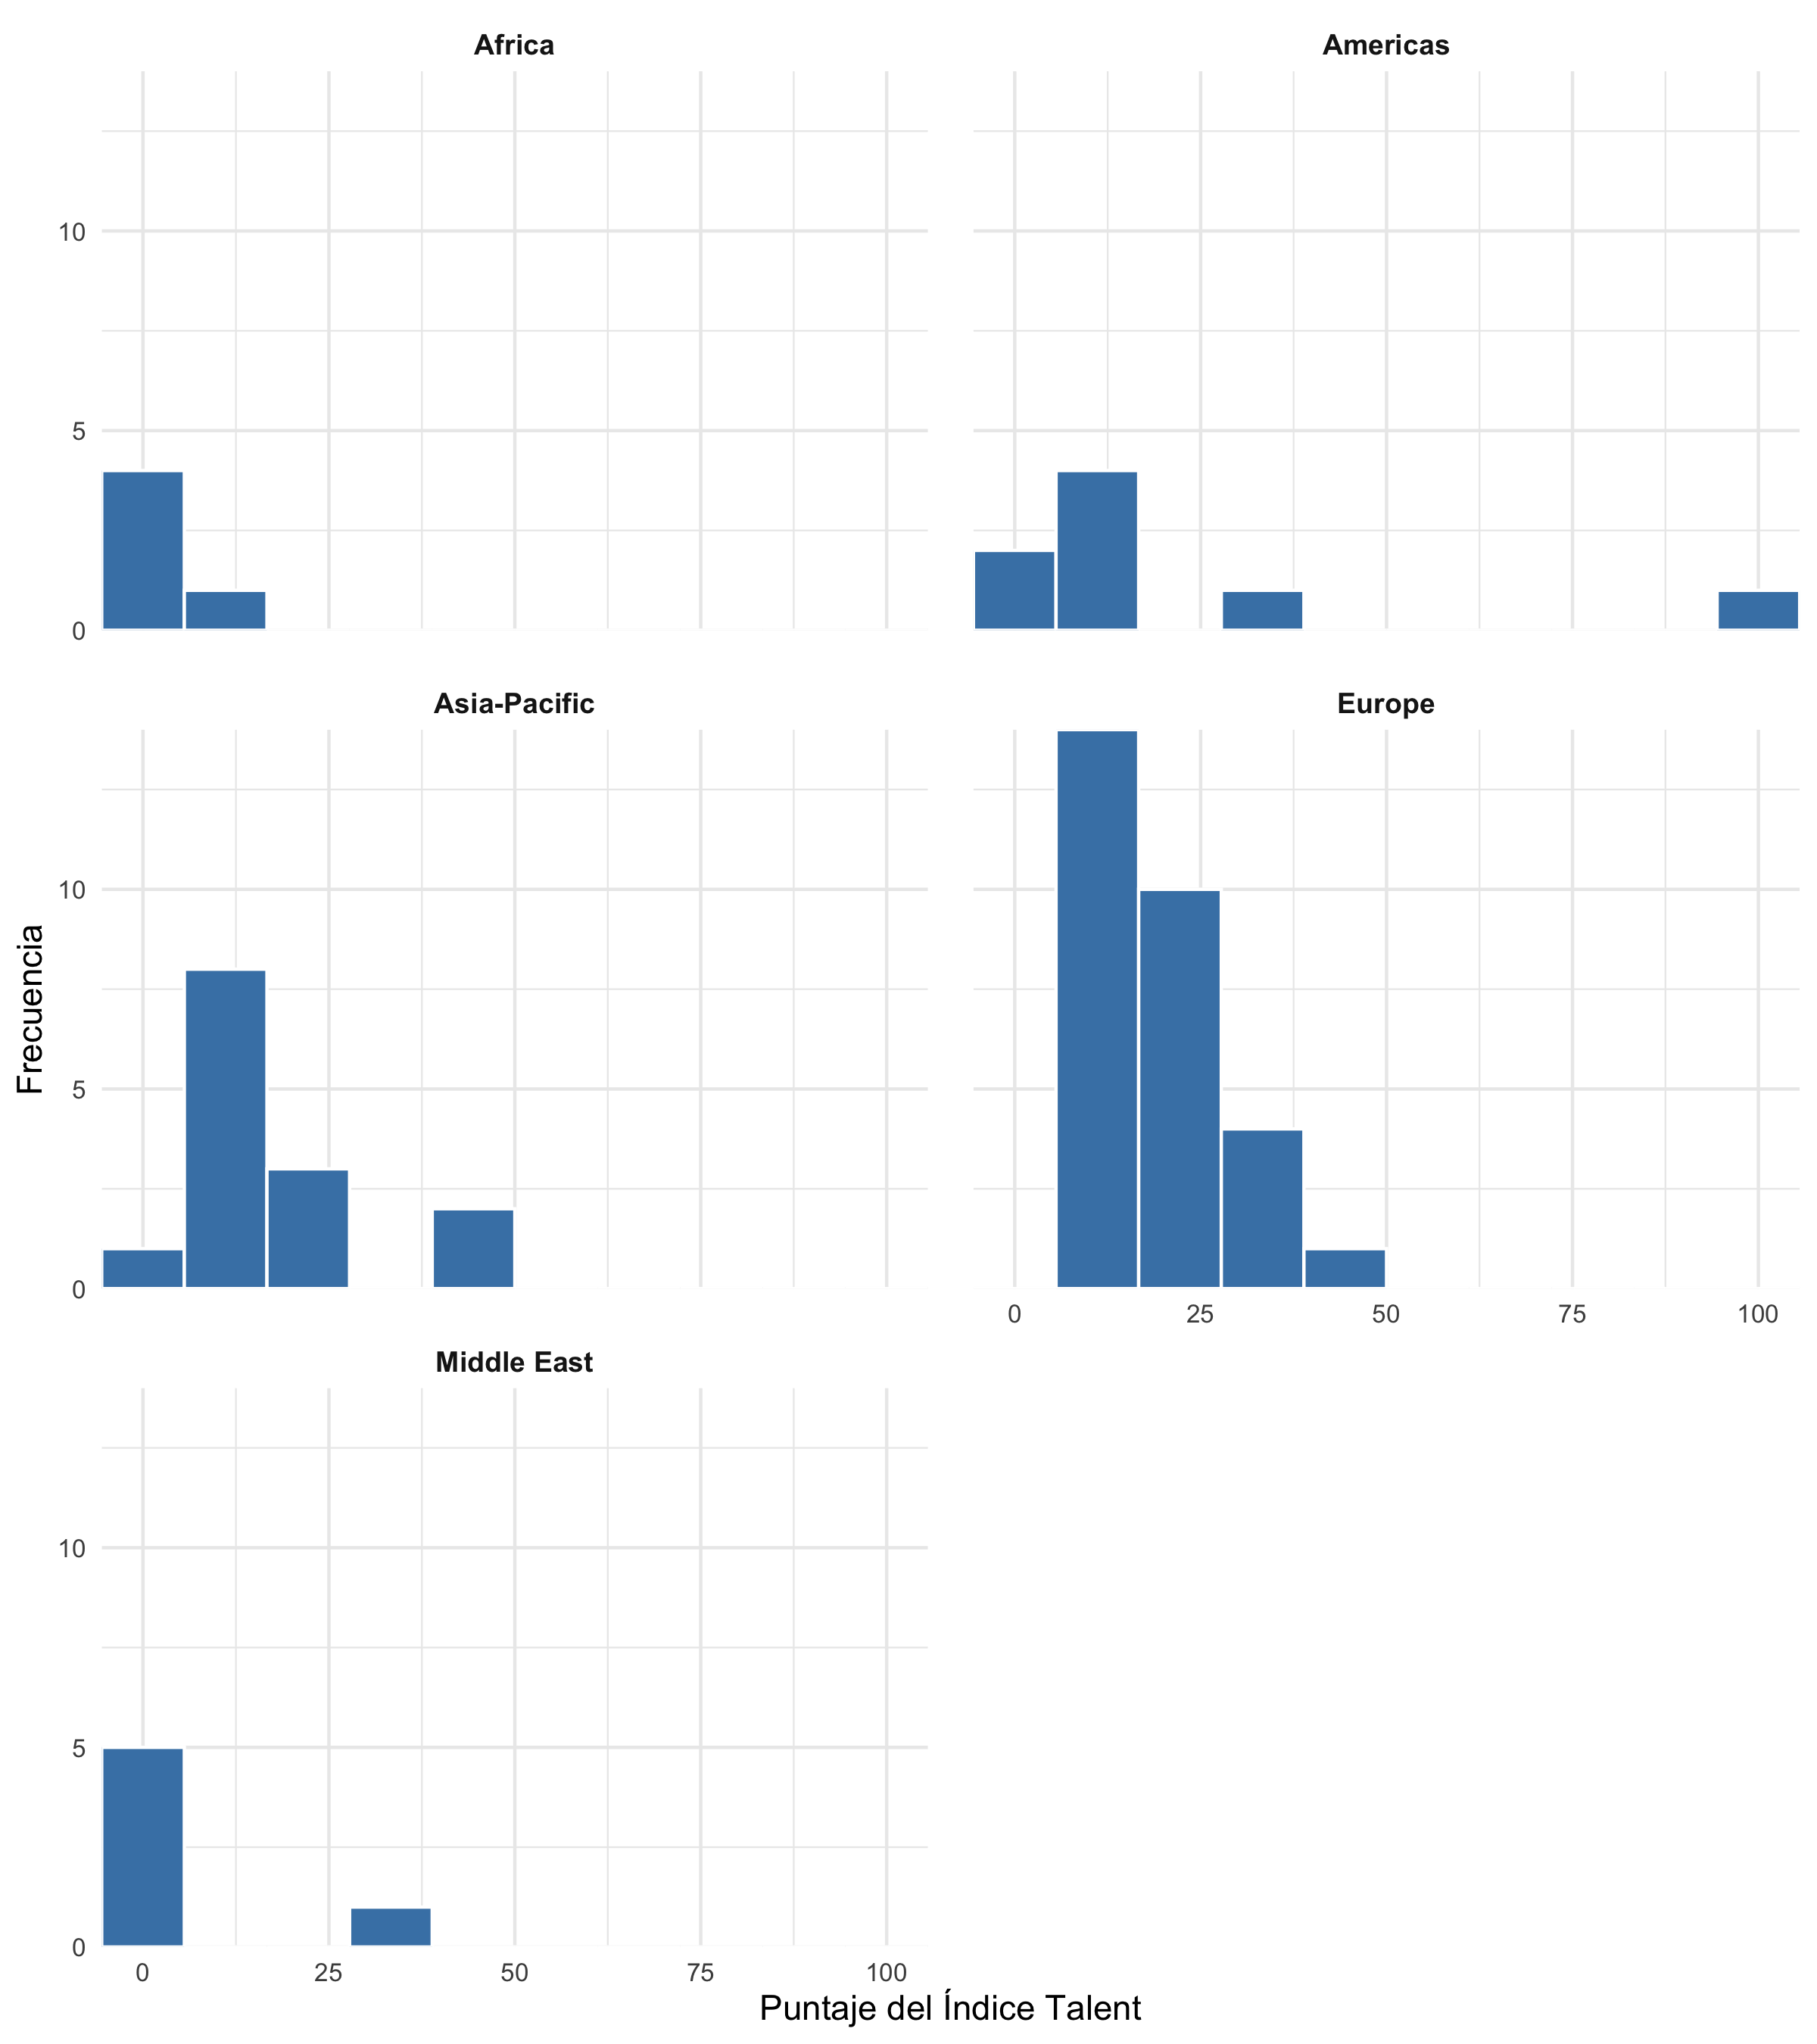
\includegraphics[width=\linewidth]{figura8.png}
\end{center}
Figura 8. Distribución del Índice Talent agrupado por Región.




\begin{center}
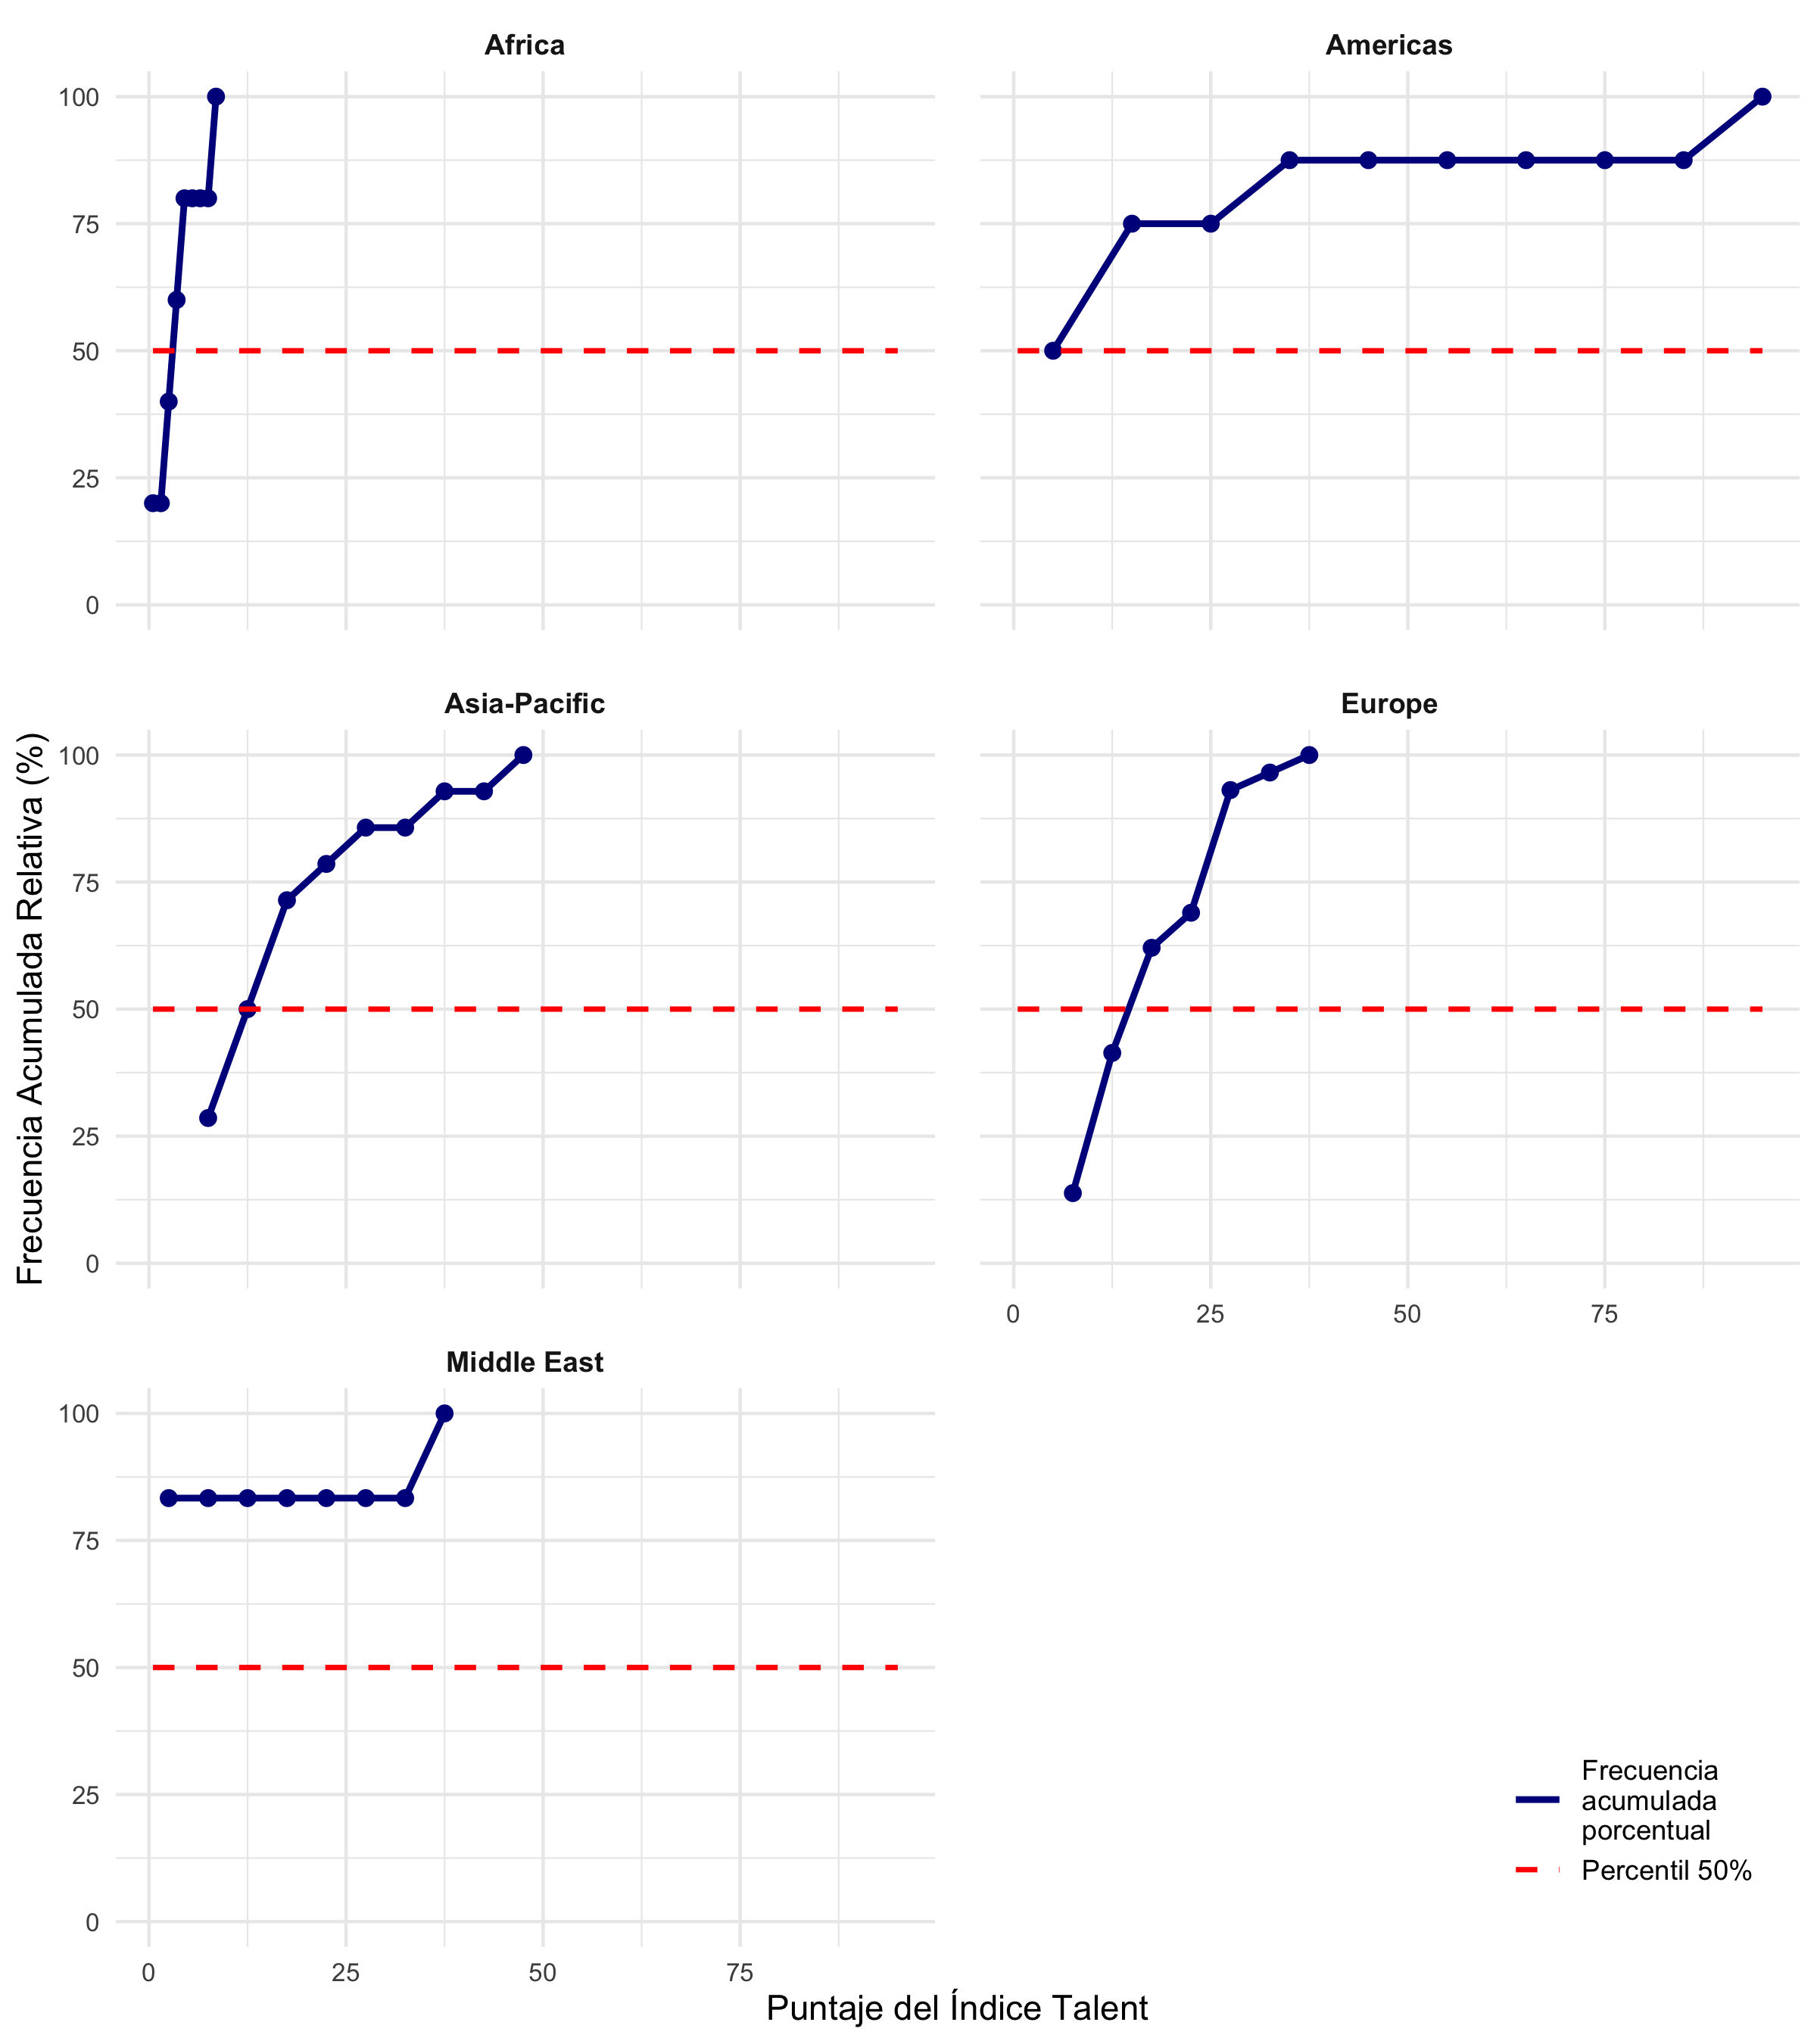
\includegraphics[width=\linewidth]{figura9.png}
\end{center}
Figura 9. Distribución acumulada del Índice Talent agrupado por Región.

\section{Intérvalos de confianza}

Al obtener una muestra aleatoria del índice Research (variable cuantitativa) con 30 datos y determinar la media de la muestra y la desviación estándar, es necesario establecer el intérvalo de confianza donde se encuentra la media real de la población.

Para obtener un intérvalo de confianza del 95\% se realizó el siguiente procedimiento:




n = 30\\
x̄ = 16.61\\
s = 10.89\\
IC = 0.95\\
IC = 1 - $\alpha$\\
$\alpha$ = 0.05\\
$\alpha$/2 = 0.025\\
Z~$\alpha$/2~ = ± 1.96\\
Márgen de error = Z~$\alpha$/2~ * s/√n\\
Márgen de error = 1.96 * 10.89/√30\\
Márgen de error = 3.8969365\\
IC = (x̄ ± Márgen de error)\\
IC = (12.71,  20.51)\\

El intérvalo presentado indica que con una probabilidad del 95\%, la media de la población se encuentra entre 12.71 y 20.51.

ESPACIO PARA VARIABLE CUALITATIVA (seguir el mismo formato)

\section{Prueba de hipótesis}



En este estudio se planteó la siguiente hipòtesis: el valor medio del índice Research (variable cuantitativa) es menor o igual a 20 puntos. Para comprobar la veracidad de la anterior afirmación con un determinado nivel de significancia, es necesario realizar una prueba de hipótesis.

A continuación se presenta la prueba de hipótesis siguiendo el método del valor crítico [4] (metodología de los 5 pasos) con el estadístico de prueba Z:

n = 30\\
x̄ = 16.61\\
s =  10.89\\

Paso 1.\\
Ho: µ $≤$ 20\\
Ha: µ > 20\\

Paso 2.\\
$\alpha$ = 0.05\\

Paso 3.\\
Z = (x̄ - µ)/(s/√n)\\
Z = ( 16.61 - 20)/(10.89/√30)\\
Z = -1.7050317\\

Paso 4.
Z crítico = Z(1 - $\alpha$)\\
Z crítico = 1.6448536\\

En la figura 10 se presenta gráficamente el posicionamiento de las regiones de rechazo y no rechazo y la ubicación de Z en las mismas.


\begin{center}
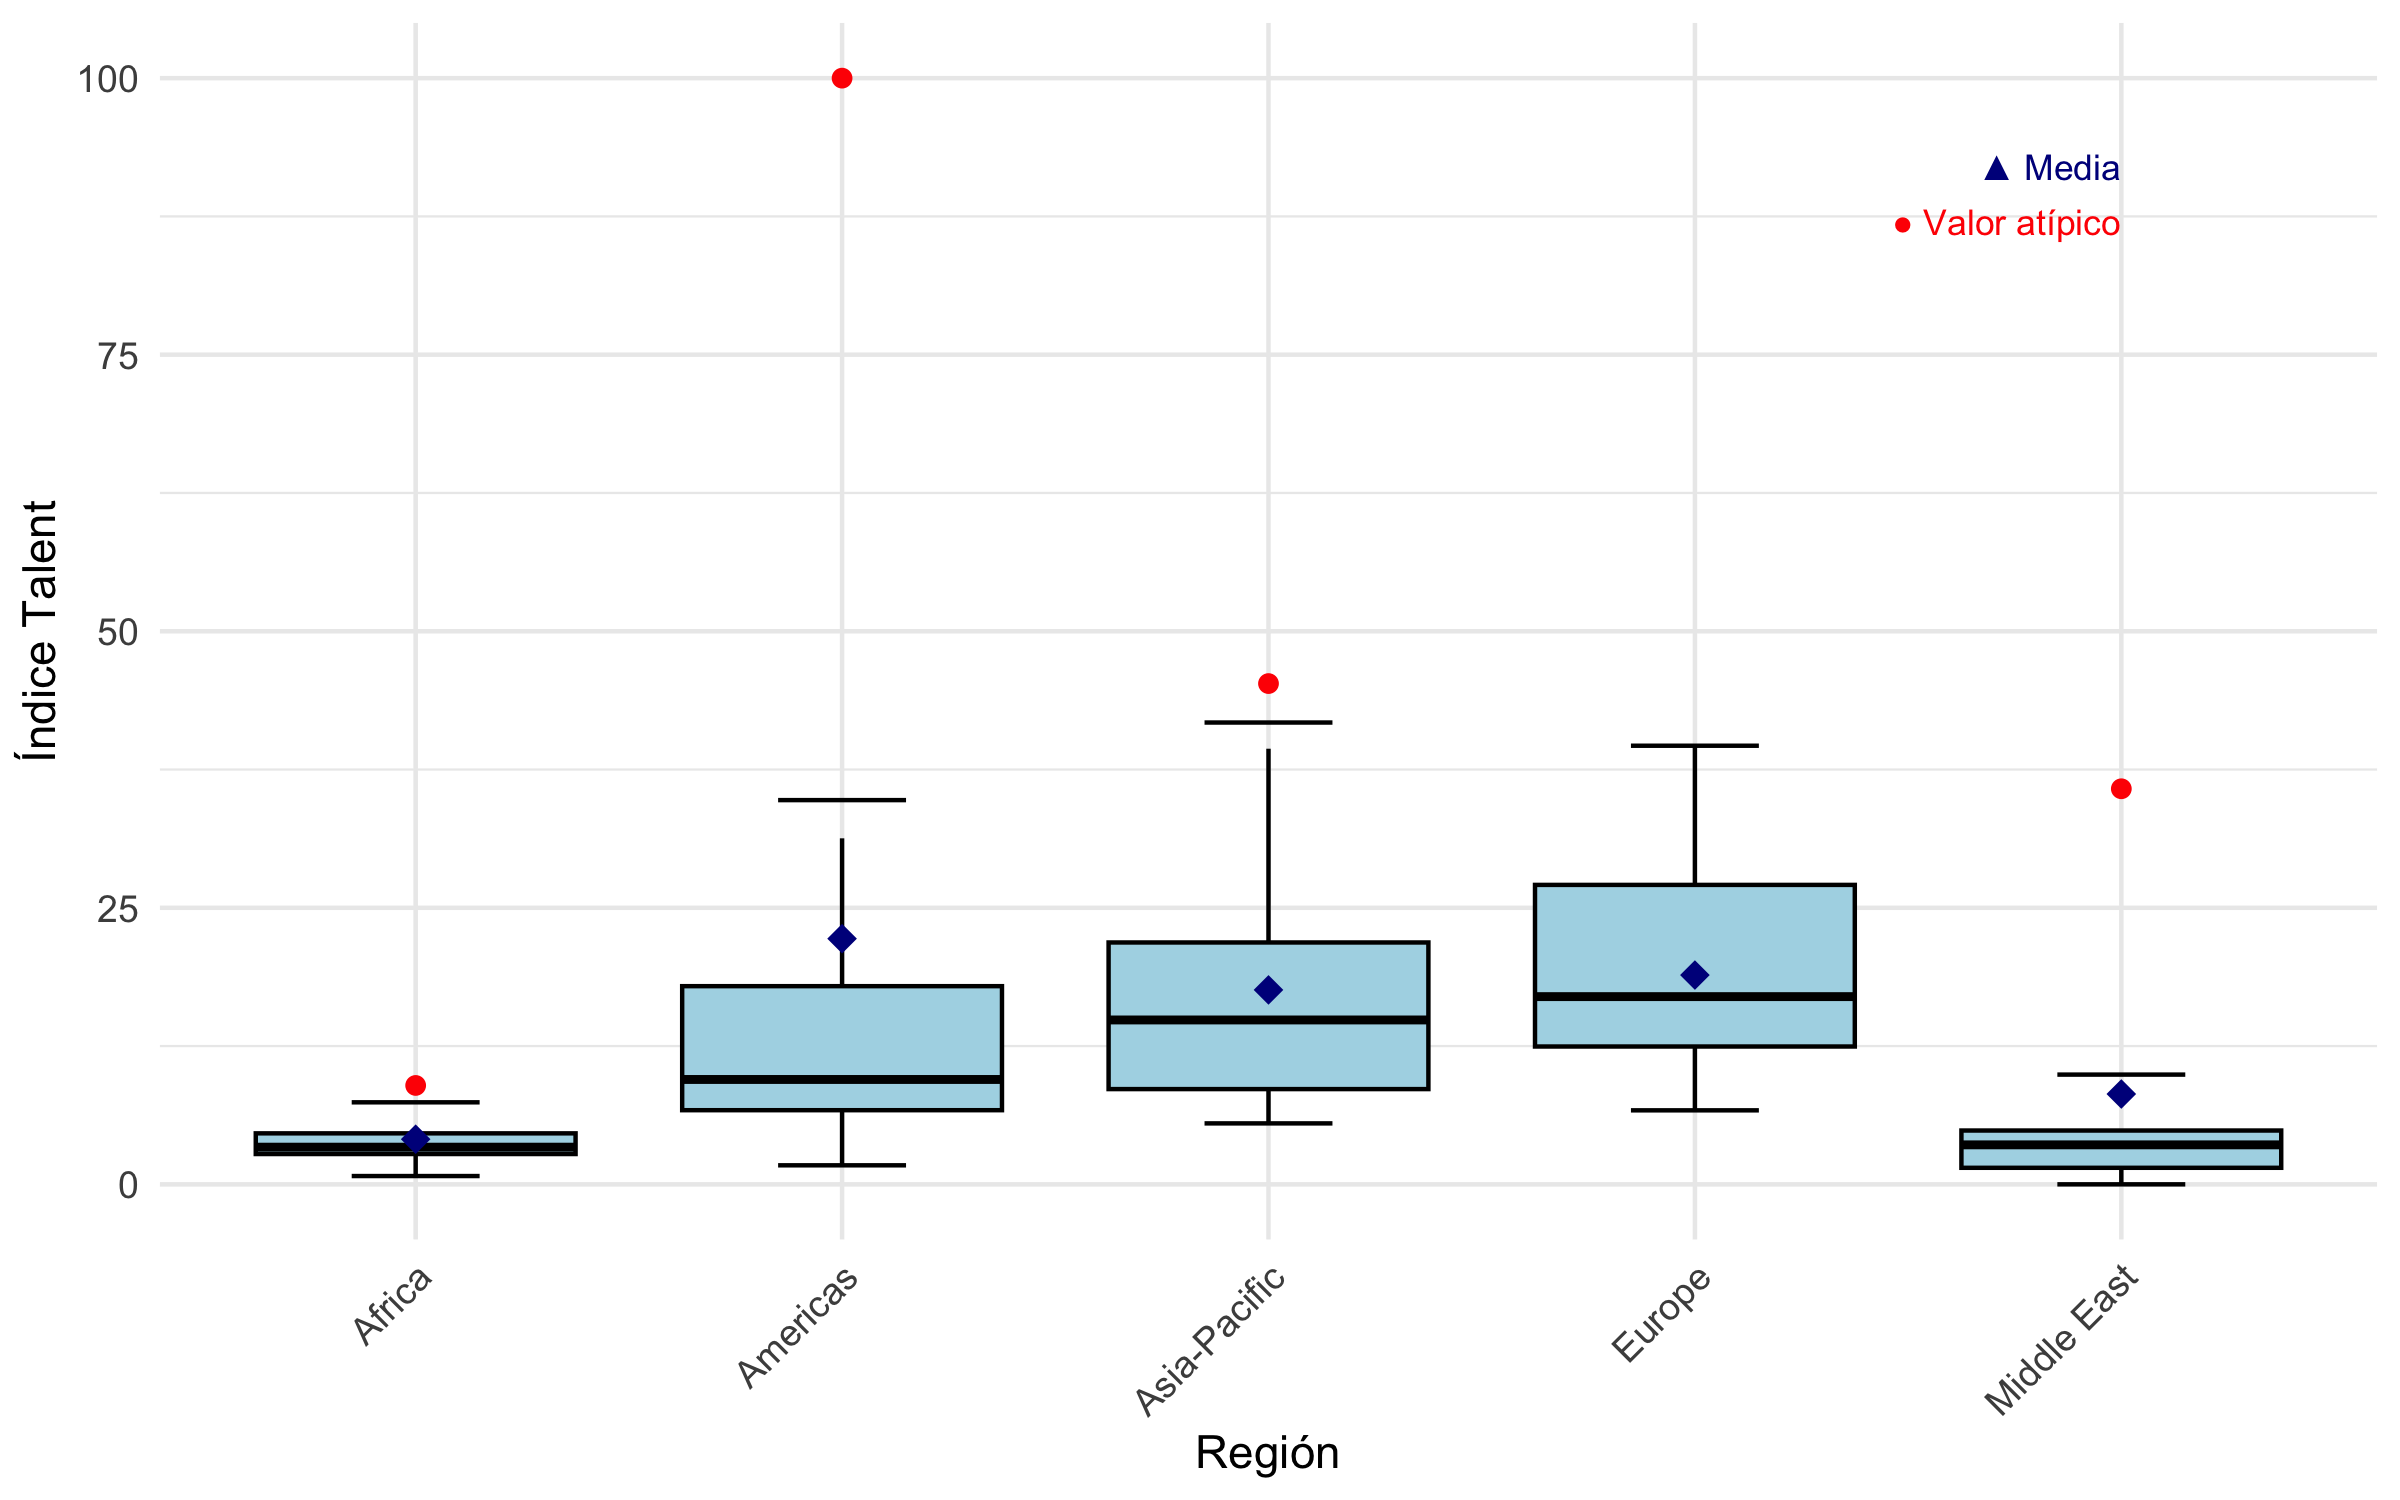
\includegraphics[width=\linewidth]{figura10.png}
\end{center}

Figura 10. Identificación de la región de rechazo

Paso 5.

Con un nivel de significancia de 0.05, se concluye que el valor medio del índice Research es menor o igual a 20 puntos, ya que no se rechaza la hipótesis nula Ho: µ $≤$ 20 debido a que Z = -1.7050317 se encuentra en la región de no rechazo (región a la izquierda de Z crítico = 1.6448536) como se aprecia en la figura 10.

ESPACIO PARA VARIABLE CUALITATIVA (seguir el mismo formato)

ESPACIO PARA DOS POBLACIONES (seguir el mismo formato)


\section{Modelo de regresión lineal simple}

Con el objetivo de determinar la influencia de los factores relacionados con la innovación mediante el índice Research en el desarrollo de la IA, se busca plantear un modelo de regresión lineal [5] simple. Para esto, se debe establecer la presencia de una relación lineal significativa (con un coeficiente de correlación lineal de Pearson $≥$ a 0.6 o $≤$ a -0.6) y visualizar la relación en un diagrama de disperción.




En la figura 11 se presenta el diagrama de disperción del índice Research y Total Score, donde se aprecia la presencia de una relación lineal entre las mismas, la cuál se ve reflejada en el coeficiente de correlación lineal de ambas variables, que es de 0.946, indicando una relación lineal directa muy significativa ya que el coeficiente es mayor a 0.6. Este análisis preliminar de la relación de las variables permite determinar que es apropiado realizar un modelo de regresión lineal de las mismas.



\begin{center}
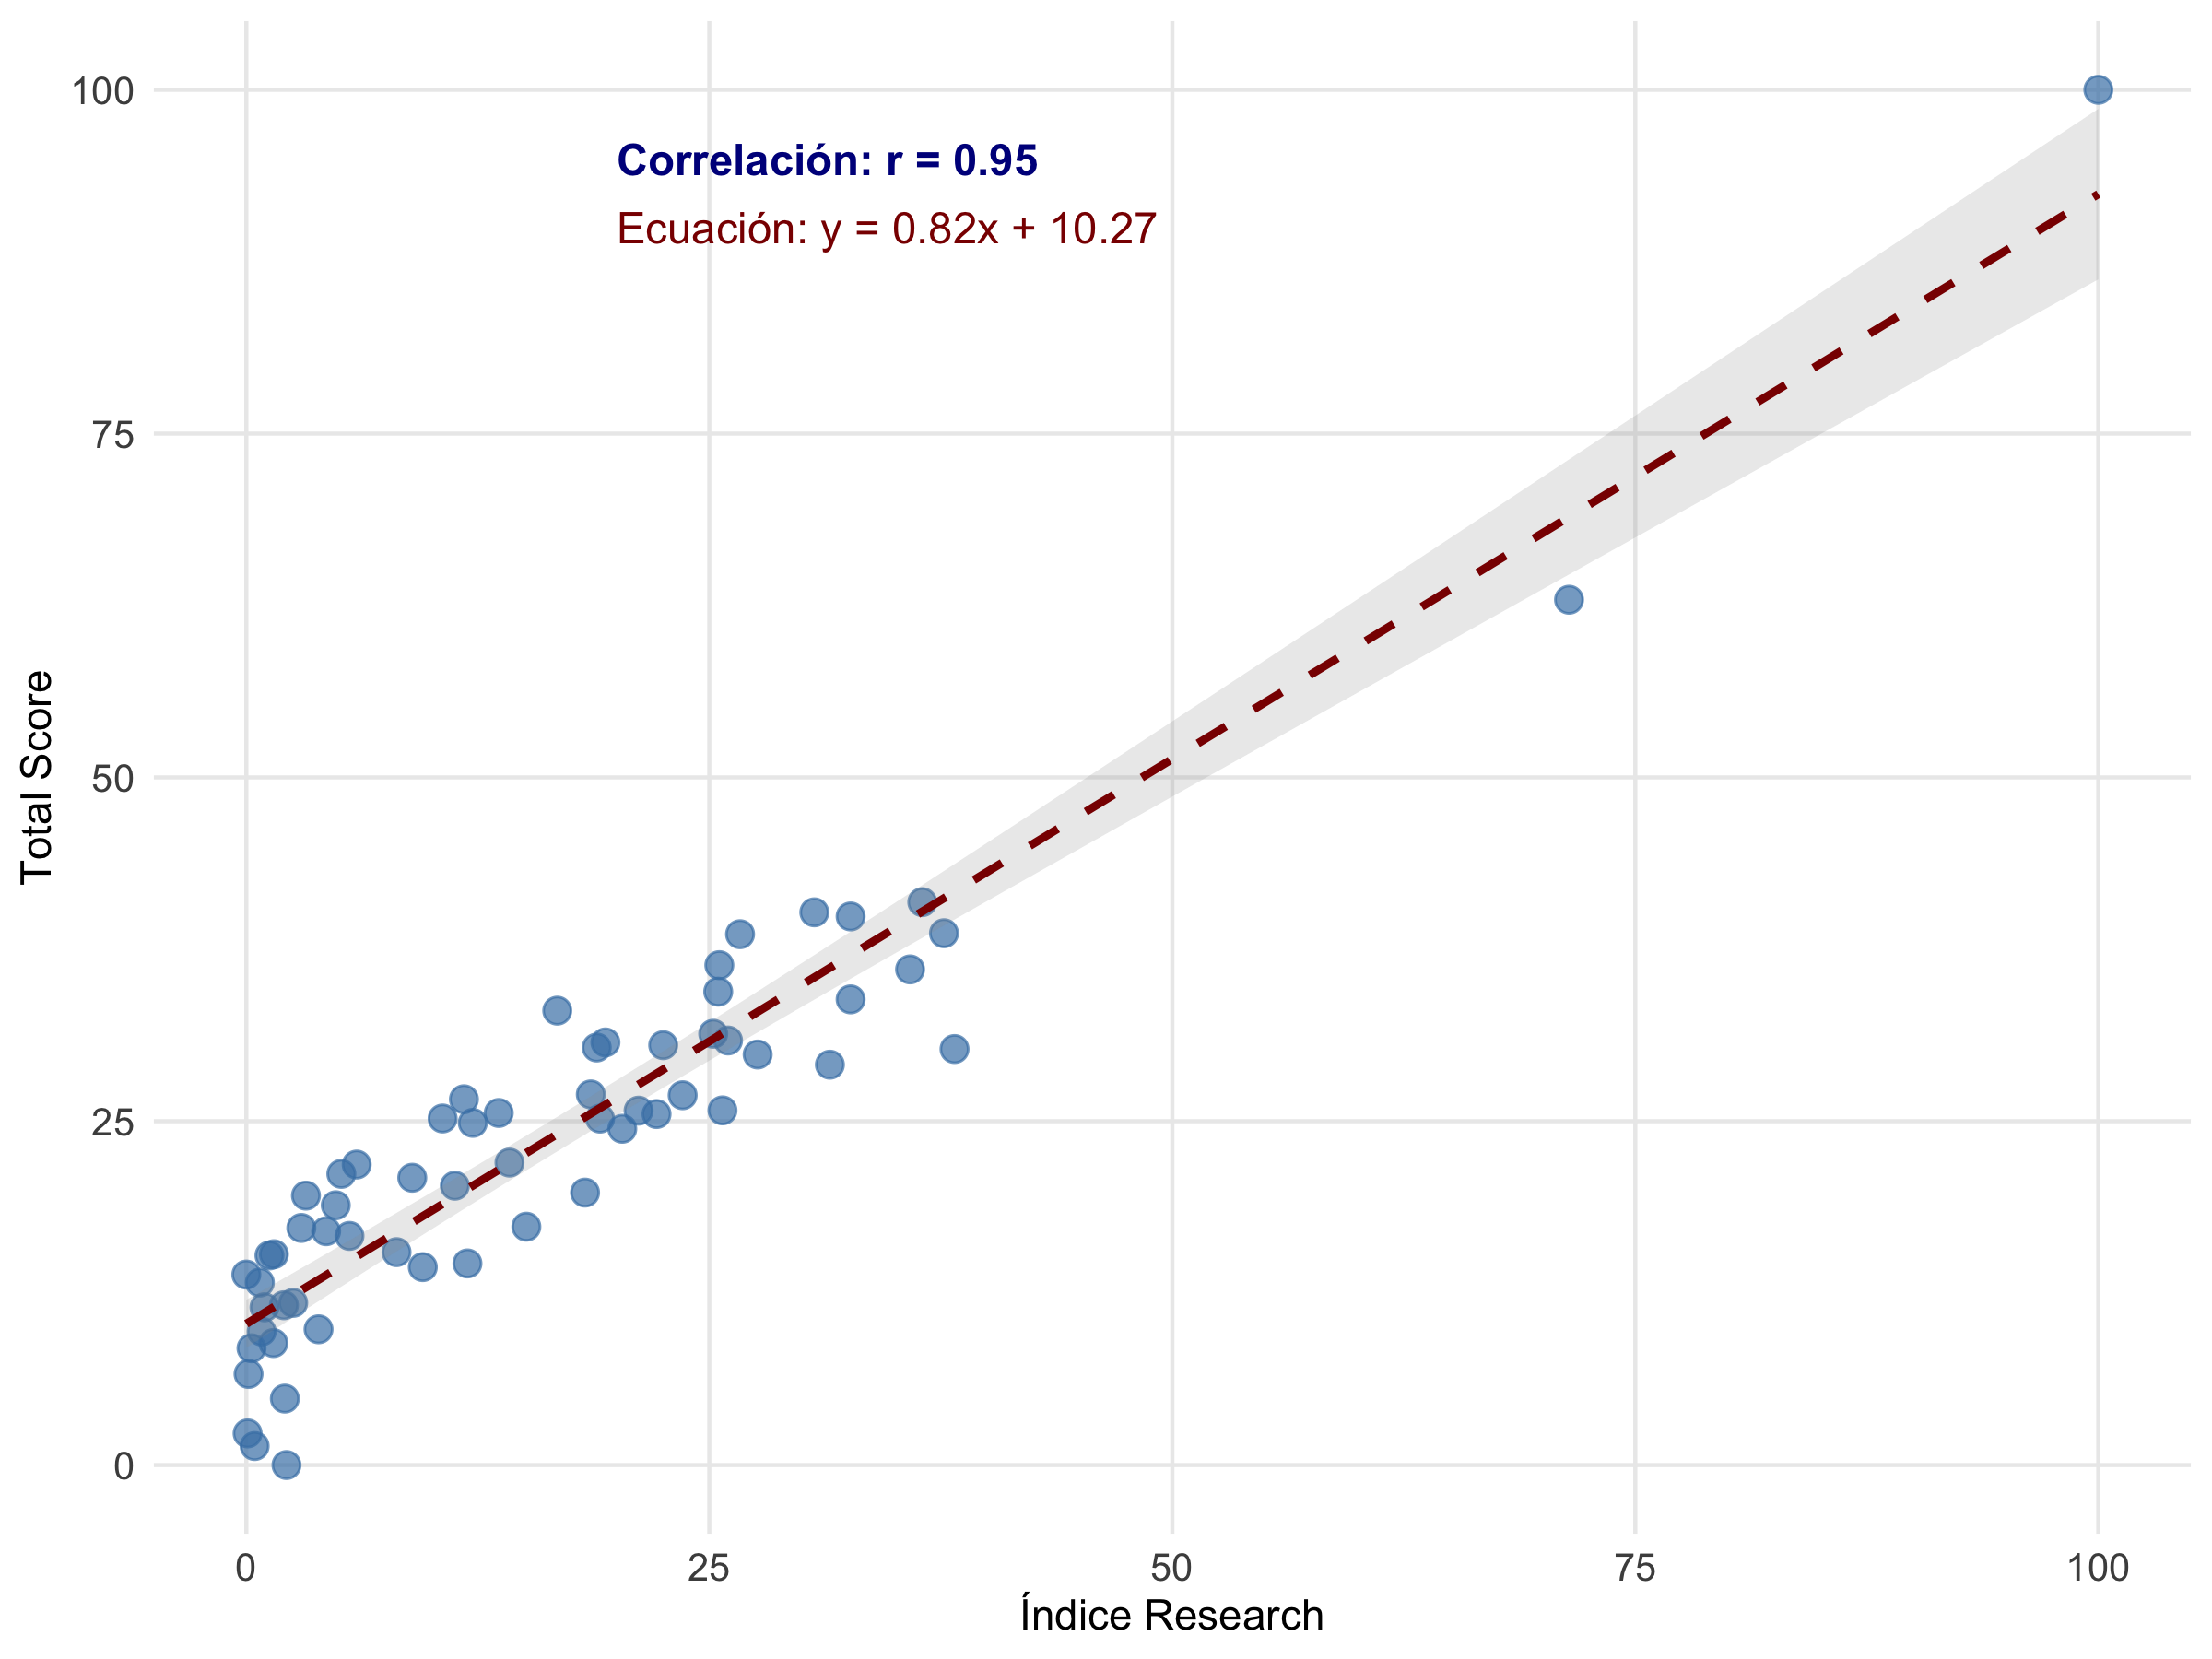
\includegraphics[width=\linewidth]{figura11.png}
\end{center}

Figura 11. Disperción de los datos del índice Research y el índice Total Score.

Las variables del modelo serán el índice Research (variable independiente X) y Total Score (variable dependiente Y). El modelo de regresión lineal es de la forma y = ßo + ß1X + $\epsilon$, donde ß0 es la ordenada de origen de la línea, ß1 es la pendiente de la línea y $\epsilon$ es un componente error aleatorio.



En la Tabla 11 se presenta una estimación de los coeficientes del modelo, el error estándar, el Valor t y el Valor p correspondiente (Pr(>|t|)). 

\begin{table}[H]
\centering
\caption{\label{tab:tabla11}Coeficientes del modelo}
\centering
\fontsize{9}{11}\selectfont
\begin{tabular}[t]{llrrr}
\toprule
  & Estimación & Error Estándar & Valor t & Valor p\\
\midrule
$\beta_0$ & 10.2701 & 0.8719 & 11.7786 & 0\\
$\beta_1$ & 0.8215 & 0.0364 & 22.5768 & 0\\
\bottomrule
\end{tabular}
\end{table}

El coeficiente ßo (intercepto) tiene un valor de  10.27 y el coeficiente ß1 tiene un valor de 0.821, generando un modelo de regresión lineal:\\

Y = ßo + ß1X + $\epsilon$\\
Y = 10.27 + 0.821* X + $\epsilon$\\
Total Score = 10.27 + 0.821 * Research + $\epsilon$\\

Para determinar la bondad del modelo se utiliza el coeficiente de determinación $R^2$ el cuál mide la exactitud de las predicciones que produce el modelo de regresión lineal, además, el coeficiente de determinación ajustado $R^2_{A}$ considera también la relación del número de parámetros con el número de datos, haciendolo más adecuado para establecer la bondad de las predicciones. A memdida que el valor de $R^2_{A}$ se acerca más a 1 se considera que el modelo es más preciso. En este caso, $R^2_{A}$ es 0.893, por lo que el 89.3\% de la variabilidad de las predicciones de Total Score pueden ser explicadas con el modelo de regresión con la variable Research.



$R^2$ = 0.8947\\
$R^2_{A}$ = 0.8929\\
Estadístico F = 509.71 con 1 y 60 grados de libertad\\
Valor p = < 2.2e-16\\

Hay 4 supuestos respecto a $\epsilon$ [6] del modelo de regrersión lineal que se deben cumplir para verificar la validez de las predicciones del modelo, estos supuestos son: 

\begin{enumerate} [itemsep=0pt, parsep=0pt]
\item Los errores $\epsilon$i son aleatorios e independientes.
\item La media de la distribución de probabilidad de  $\epsilon$ es 0.
\item La varianza de la distribución de probabilidad de  $\epsilon$ es constante para todos los valores de la variable independiente X (índice Research).
\item Los  $\epsilon$i están distribuidos normalmente.
\end{enumerate}

Para comprobar el primer supuesto, en la figura 12 se presenta un diagrama de disperción de los residuos de los pronósticos para Total Score, donde se evidencia que estos no mantienen una relación evidente entre sí, de tal manera que se cumple el supuesto 1.


\begin{center}
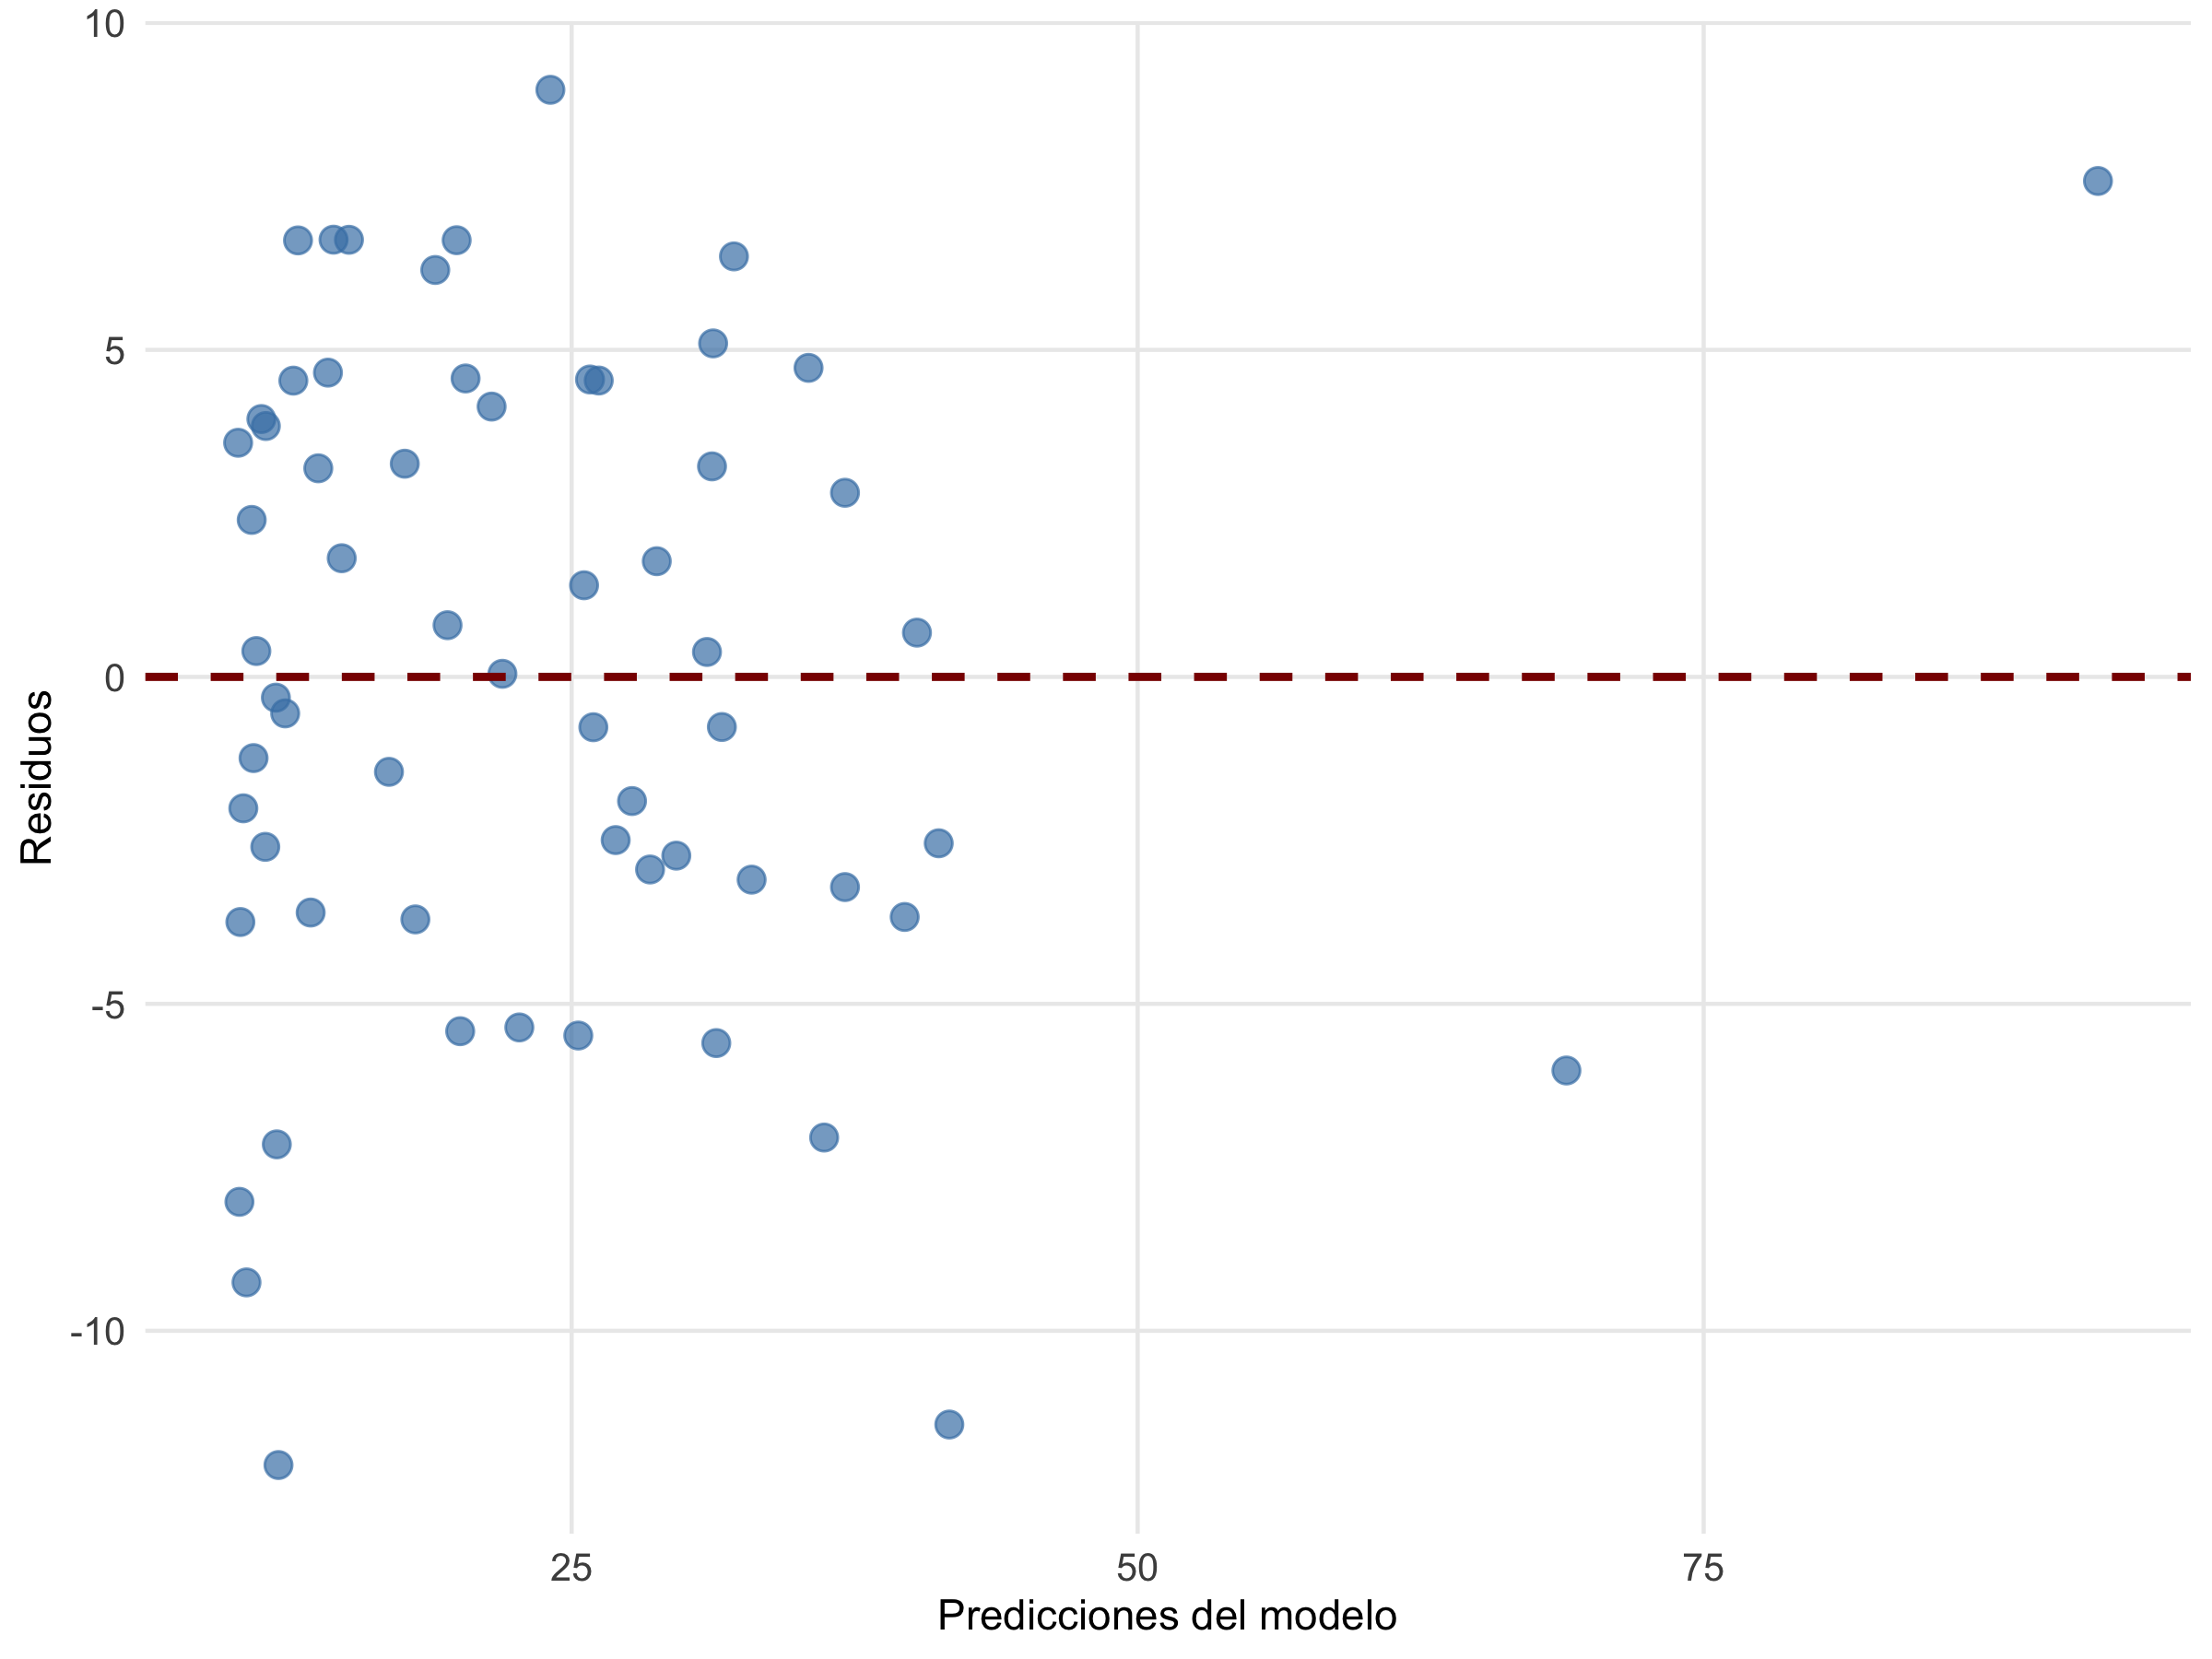
\includegraphics[width=\linewidth]{figura12.png}
\end{center}

Figura 12. Disperción de los residuos de los pronósticos de Total Score.



Para comporbar el segundo supuesto, se calculó la media de la distribución de probabilidad de $\epsilon$, esta es de \ensuremath{1.1323268\times 10^{-16}}, la cuál redondeada a 6 decimales es de aproximadamente 0.

Para comprobar el tercer supuesto Homocedasticidad [7], en la Tabla 12 se plantea el análisis de varianza ANOVA, con el cual se buscará probar la hipótesis: existe una relación lineal significativa entre el índice Research y Total Score.




n = 62\\
Paso 1.\\
Ho: ß1 = 0\\
Ha: ß1 $≠$ 0\\

Paso 2.\\
$\alpha$ = 0.05

Paso 3.\\
F = 509.7109065\\

Paso 4.\\
Valor p = \ensuremath{5.1203653\times 10^{-31}}\\
alfa - Valor p = 0.05\\
Valor p < $\alpha$

Paso 5.
Con una significancia de 0.05, se rechaza la hipótesis nula ya que el Valor p \ensuremath{5.1203653\times 10^{-31}} es menor a  $\alpha$, por lo tanto se concluye ß1 $≠$ 0 y por lo tanto existe una relación lineal significativa entre el índice Research y Total Score.


\end {multicols}

\renewcommand{\arraystretch}{1.3}
\begin{footnotesize}
\begin{longtable}[t]{lcrrrr}
\caption{\label{tab:tabla12}Análisis de Varianza (ANOVA) para el Modelo de Regresión Lineal}\\
\toprule
Fuente de Variación & Grados de Libertad & Suma de Cuadrados & Cuadrado medio & F & Valor P\\
\midrule
Regresión & 1 & 12482.71 & 12482.71 & 509.71 & < 2.2e-16\\
Error (residuo) & 60 & 1469.39 & 24.49 & NA & NA\\
Total & 61 & 13952.09 & NA & NA & NA\\
\bottomrule
\end{longtable}

\end{footnotesize}\renewcommand{\arraystretch}{1}

\begin{multicols}{2}

Al comprobar la hipítesis planteada: existe una relación lineal significativa entre el índice Research y Total Score, utilizando el análisis de varianza ANOVA para el mdelo de regresión lineal, se determina el cumplimiento del tercer supuesto del modelo

En la figura 13 se presenta la distribución de los residuos de los pronósticos de Total Score para comprobar el cuarto supuesto. Se observa que aunque no se muestran asimetrías muy significativas, la distribución presenta dos picos en los residuos (distribución bimodal) de manera que el supuesto de normalidad no se cumple estrictamente, sin embargo de manera general hay una distribución con similutud significativa a la curva normal.


\begin{center}
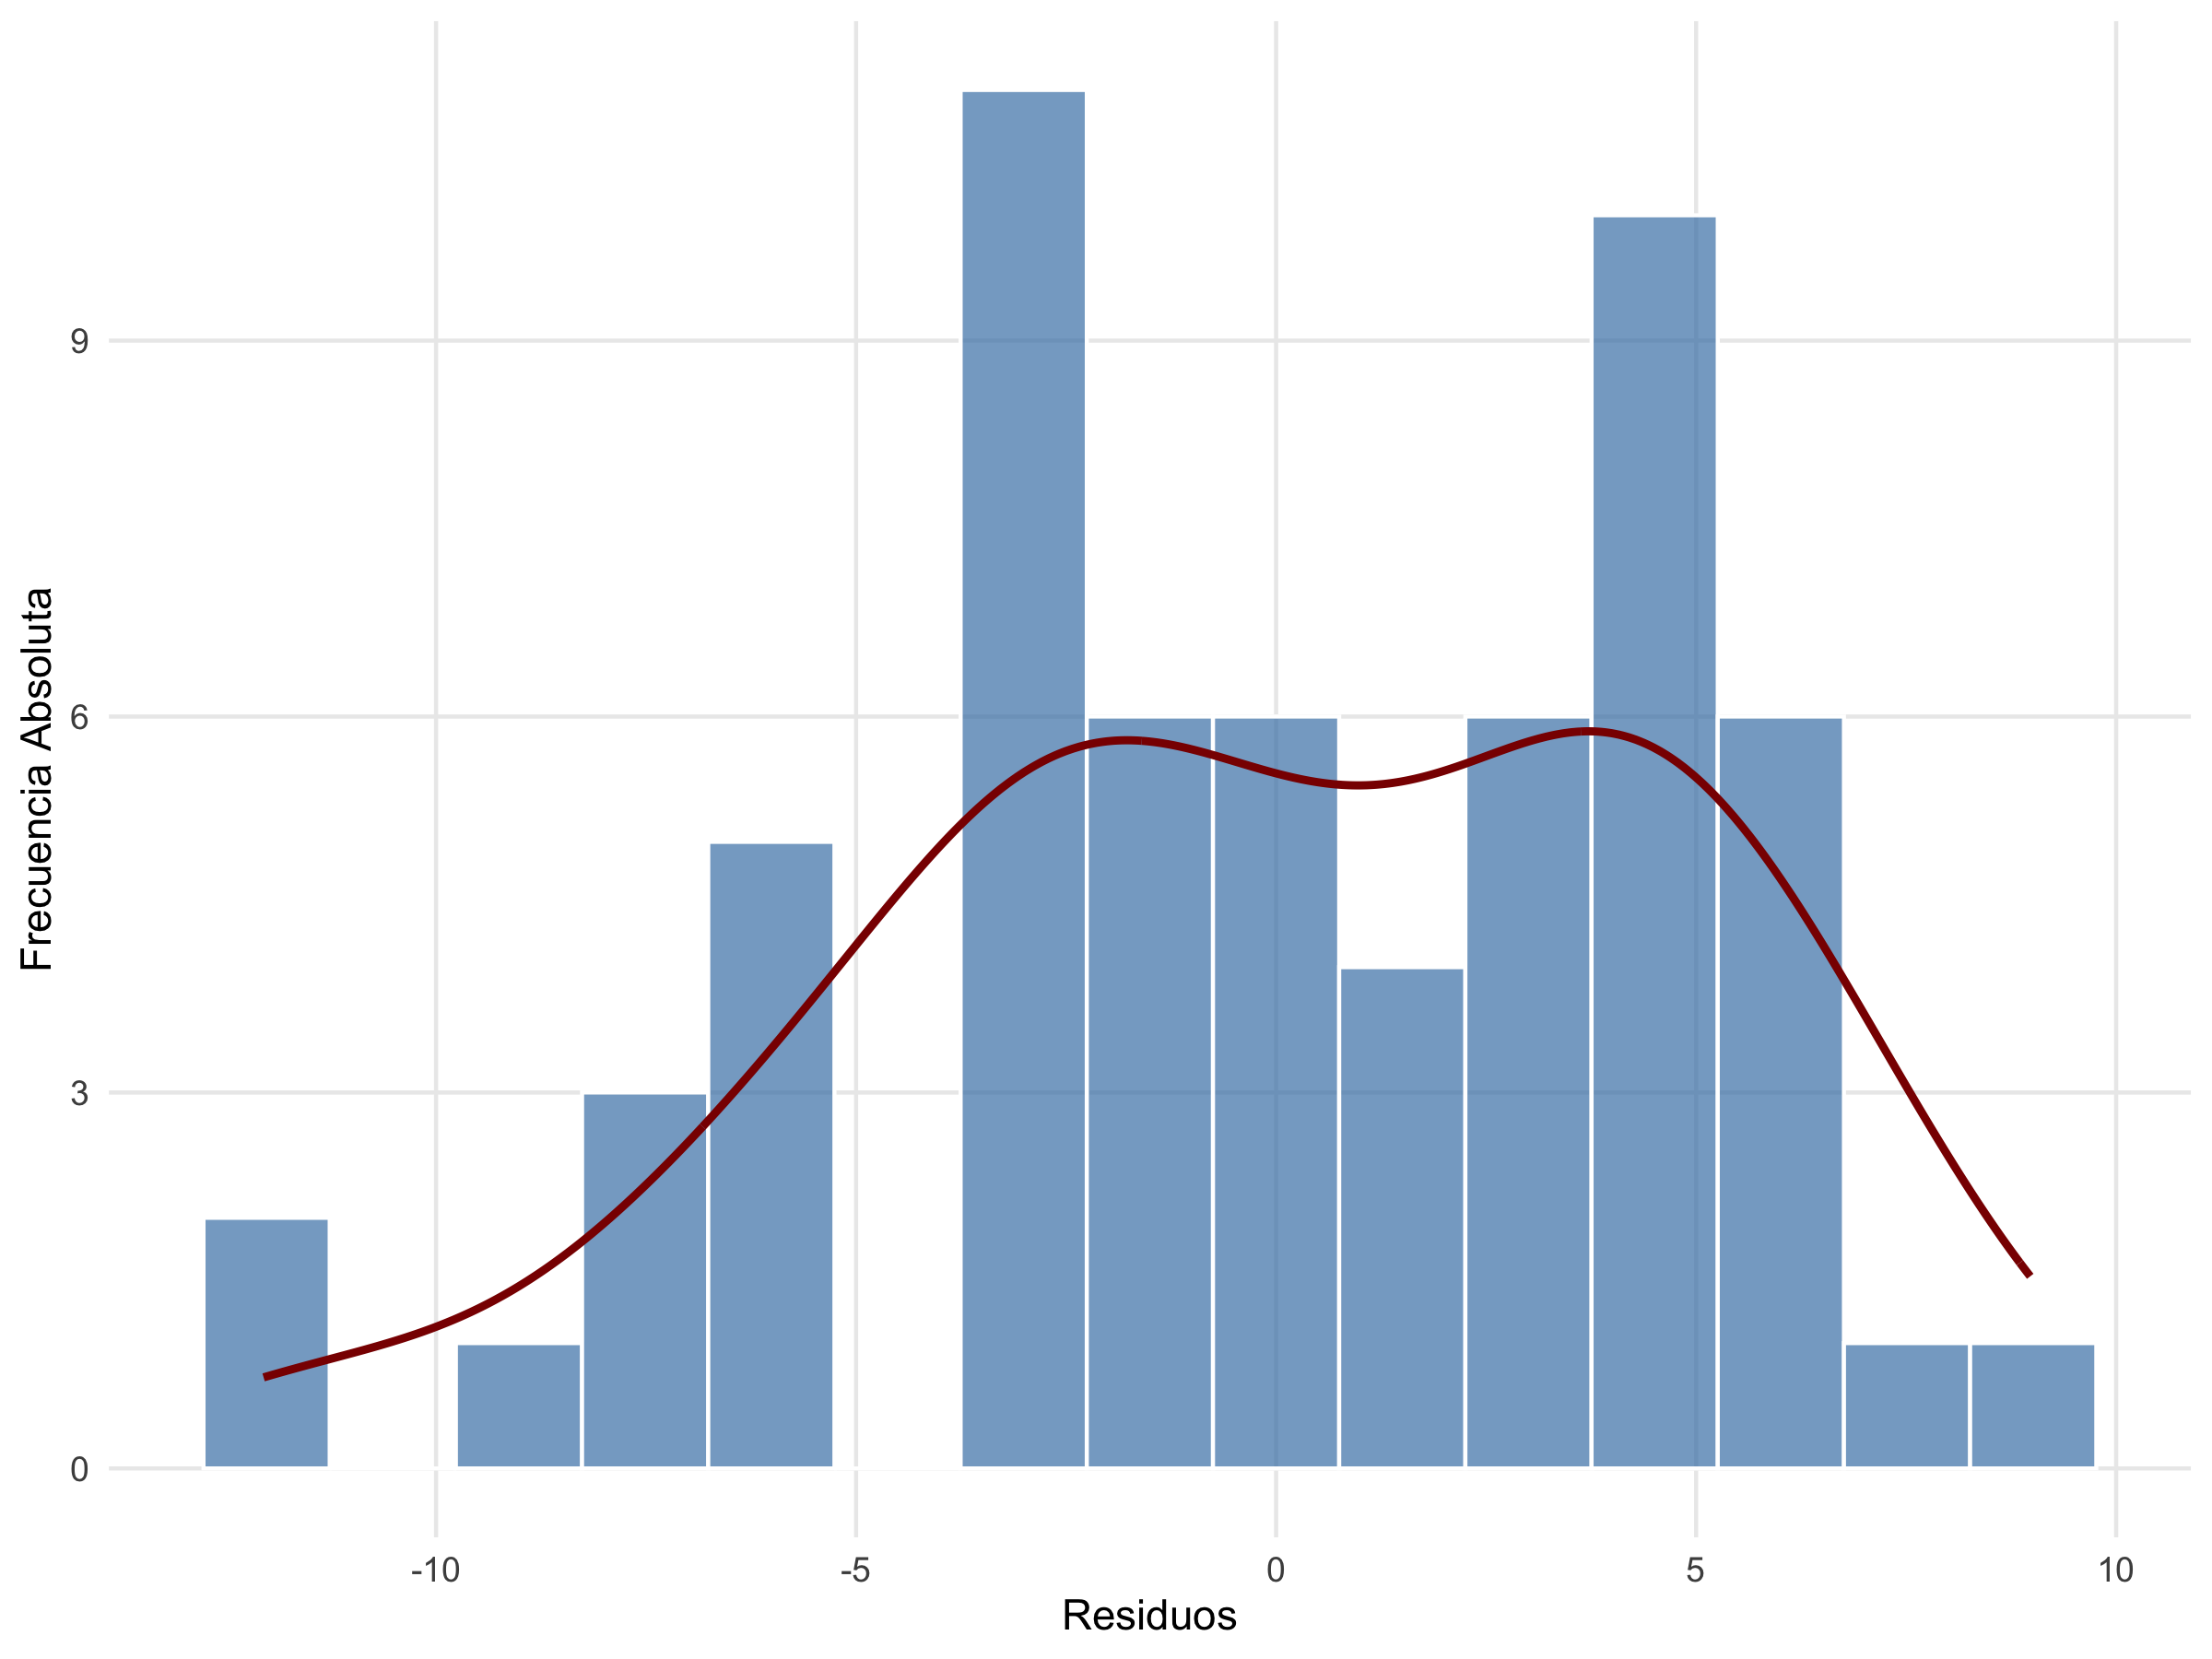
\includegraphics[width=\linewidth]{figura13.png}
\end{center}

Figura 13. Distribución los residuos de los pronósticos de Total Score.




Con el fin de comprobar la fiabilidad del modelo, en primera instancia, se observa gráficamente en la Figura 11 y se identifica a través del coeficiente de correlación lineal de Pearson que hay una relación lineal muy significativa de 0.946 entre las variables índice Research y Total Score. Por otro lado, la bondad del modelo medida por el coeficiente de determinación es de 0.893, valor que brinda una alta confiabilidad a las predicciones del modelo, indicando que el 89.3\% de la variabilidad de las predicciones de Total Score pueden ser explicadas con el modelo de regresión lineal mediante la variable Research. Es necesario considerar que las predicciones de un modelo solo son válidas dentro del rango de la muestra estudiada, en este caso, esta corresponde a (0 - 100). Debido a que el rango de las muestras coincide con el rango de los resultados posibles (0 - 100), es válido realizar predicciones  para Total Score con cualquier valor del índice Research. Finalmente debido al cumplimiento de los supuestos probado anteriormente, puede considerarse fiable pronosticar con el modelo construido.

\subsection{Modelo de Regresión Lineal Múltiple}

El modelo de regresión lineal múltiple permite analizar el efecto conjunto de varias variables explicativas sobre una variable dependiente continua. A diferencia del modelo simple, en este caso se consideran múltiples factores al mismo tiempo, lo cual ofrece una visión más completa del fenómeno estudiado. En el contexto del presente trabajo, se busca explicar el comportamiento del \textbf{Total Score}, un indicador que resume el desempeño global en inteligencia artificial de diferentes países.

Se plantea entonces un modelo de la forma:

\[
Y = \beta_0 + \beta_1 X_1 + \beta_2 X_2 + \beta_3 X_3 + \varepsilon
\]

Donde:

\begin{itemize}
  \item \( Y \): \textbf{Total Score}, la variable dependiente (indicador global de IA),
  \item \( X_1 \): \textbf{Commerce}, representa el nivel de inversión en IA,
  \item \( X_2 \): \textbf{Research}, mide la capacidad investigativa e innovación,
  \item \( X_3 \): \textbf{Talent}, refleja la disponibilidad y formación de talento humano,
  \item \( \varepsilon \): término de error aleatorio, que captura factores no observados.
\end{itemize}

Este tipo de modelo permite controlar simultáneamente por el efecto de distintas variables, mejorando la precisión de las estimaciones y evitando atribuir a una sola variable un efecto que puede estar compartido o explicado por otras.

A continuación se ajusta el modelo utilizando los datos disponibles:

\begin{table}[H]
\centering
\caption{\label{tab:modelo_multip_fit_clean}Tabla. Coeficientes estimados del modelo de regresión múltiple}
\centering
\resizebox{\ifdim\width>\linewidth\linewidth\else\width\fi}{!}{
\fontsize{9}{11}\selectfont
\begin{tabular}[t]{llrrr}
\toprule
  & Estimación & Error Estándar & Valor t & Valor p\\
\midrule
(Intercept) & 9.6347 & 0.9661 & 9.9728 & 0.0000\\
Commercial & 0.1145 & 0.0784 & 1.4607 & 0.1495\\
Research & 0.5711 & 0.0653 & 8.7414 & 0.0000\\
Talent & 0.2432 & 0.0655 & 3.7147 & 0.0005\\
\bottomrule
\end{tabular}}
\end{table}

El modelo ajustado presenta un coeficiente de determinación \( R^2 = 0.9241\), y un \( R^2_{ajustado} = 0.9201\), lo que indica un alto poder explicativo. La prueba global F arroja un valor de \( F = 235.28\), con gl = 3 y 58, y un valor-p \( p < 0.001 \), lo que confirma que el modelo es estadísticamente significativo.
Los coeficientes estimados del modelo indican el efecto promedio que tiene cada una de las variables explicativas sobre el Total Score, manteniendo las demás constantes. En otras palabras, muestran cuánto se espera que varíe el puntaje total cuando una de las variables se incrementa en una unidad, suponiendo que las demás no cambian.

Estos coeficientes, junto con sus errores estándar y valores p, permiten evaluar qué tan significativos son los efectos estimados y en qué medida contribuyen al modelo. Esta información se presenta en la siguiente tabla:


\subsubsection{Prueba de hipótesis (ANOVA)}

Se aplica ANOVA para comprobar si el modelo completo es significativo.

\begin{itemize}
  \item Paso 1. \( H_0: \beta_1 = \beta_2 = \beta_3 = 0 \), \quad \( H_a: \) al menos uno \( \beta_i \neq 0 \)
  \item Paso 2. \( \alpha = 0.05 \)
\end{itemize}

\end{multicols}

\renewcommand{\arraystretch}{1.3}
\begin{footnotesize}
\begin{longtable}[t]{llcrrrr}
\caption{\label{tab:modelo_multip_anova}Tabla. Análisis de varianza (ANOVA) del modelo múltiple}\\
\toprule
  & Fuente & GL & Suma de Cuadrados & Cuadrado Medio & F & Valor P\\
\midrule
Commercial & Commercial & 1 & 10270.6716 & 10270.6716 & 562.2828 & 0e+00\\
Research & Research & 1 & 2369.9383 & 2369.9383 & 129.7457 & 0e+00\\
Talent & Talent & 1 & 252.0546 & 252.0546 & 13.7991 & 5e-04\\
Residuals & Residuals & 58 & 1059.4294 & 18.2660 & NA & NA\\
\bottomrule
\end{longtable}

\end{footnotesize}\renewcommand{\arraystretch}{1}

\begin{multicols}{2}

Como el valor p es menor a 0.05, se rechaza \( H_0 \), concluyendo que el modelo tiene utilidad estadística global.

\subsubsection{Evaluación del ajuste y supuestos}

[1] "R² ajustado: 0.9201"

Los residuos cumplen con los supuestos del modelo:

\begin{enumerate}
  \item Son independientes.
  \item Tienen media cercana a cero.
  \item Tienen varianza constante (homocedasticidad).
  \item Están aproximadamente distribuidos normalmente.
\end{enumerate}

\textbf{Conclusión:}  
Dado que el modelo es estadísticamente significativo, con buen ajuste (\( R^2 \) alto) y supuestos cumplidos, \textbf{sí se puede utilizar para hacer predicciones confiables}, siempre dentro del rango observado de los datos.





\begin{center}
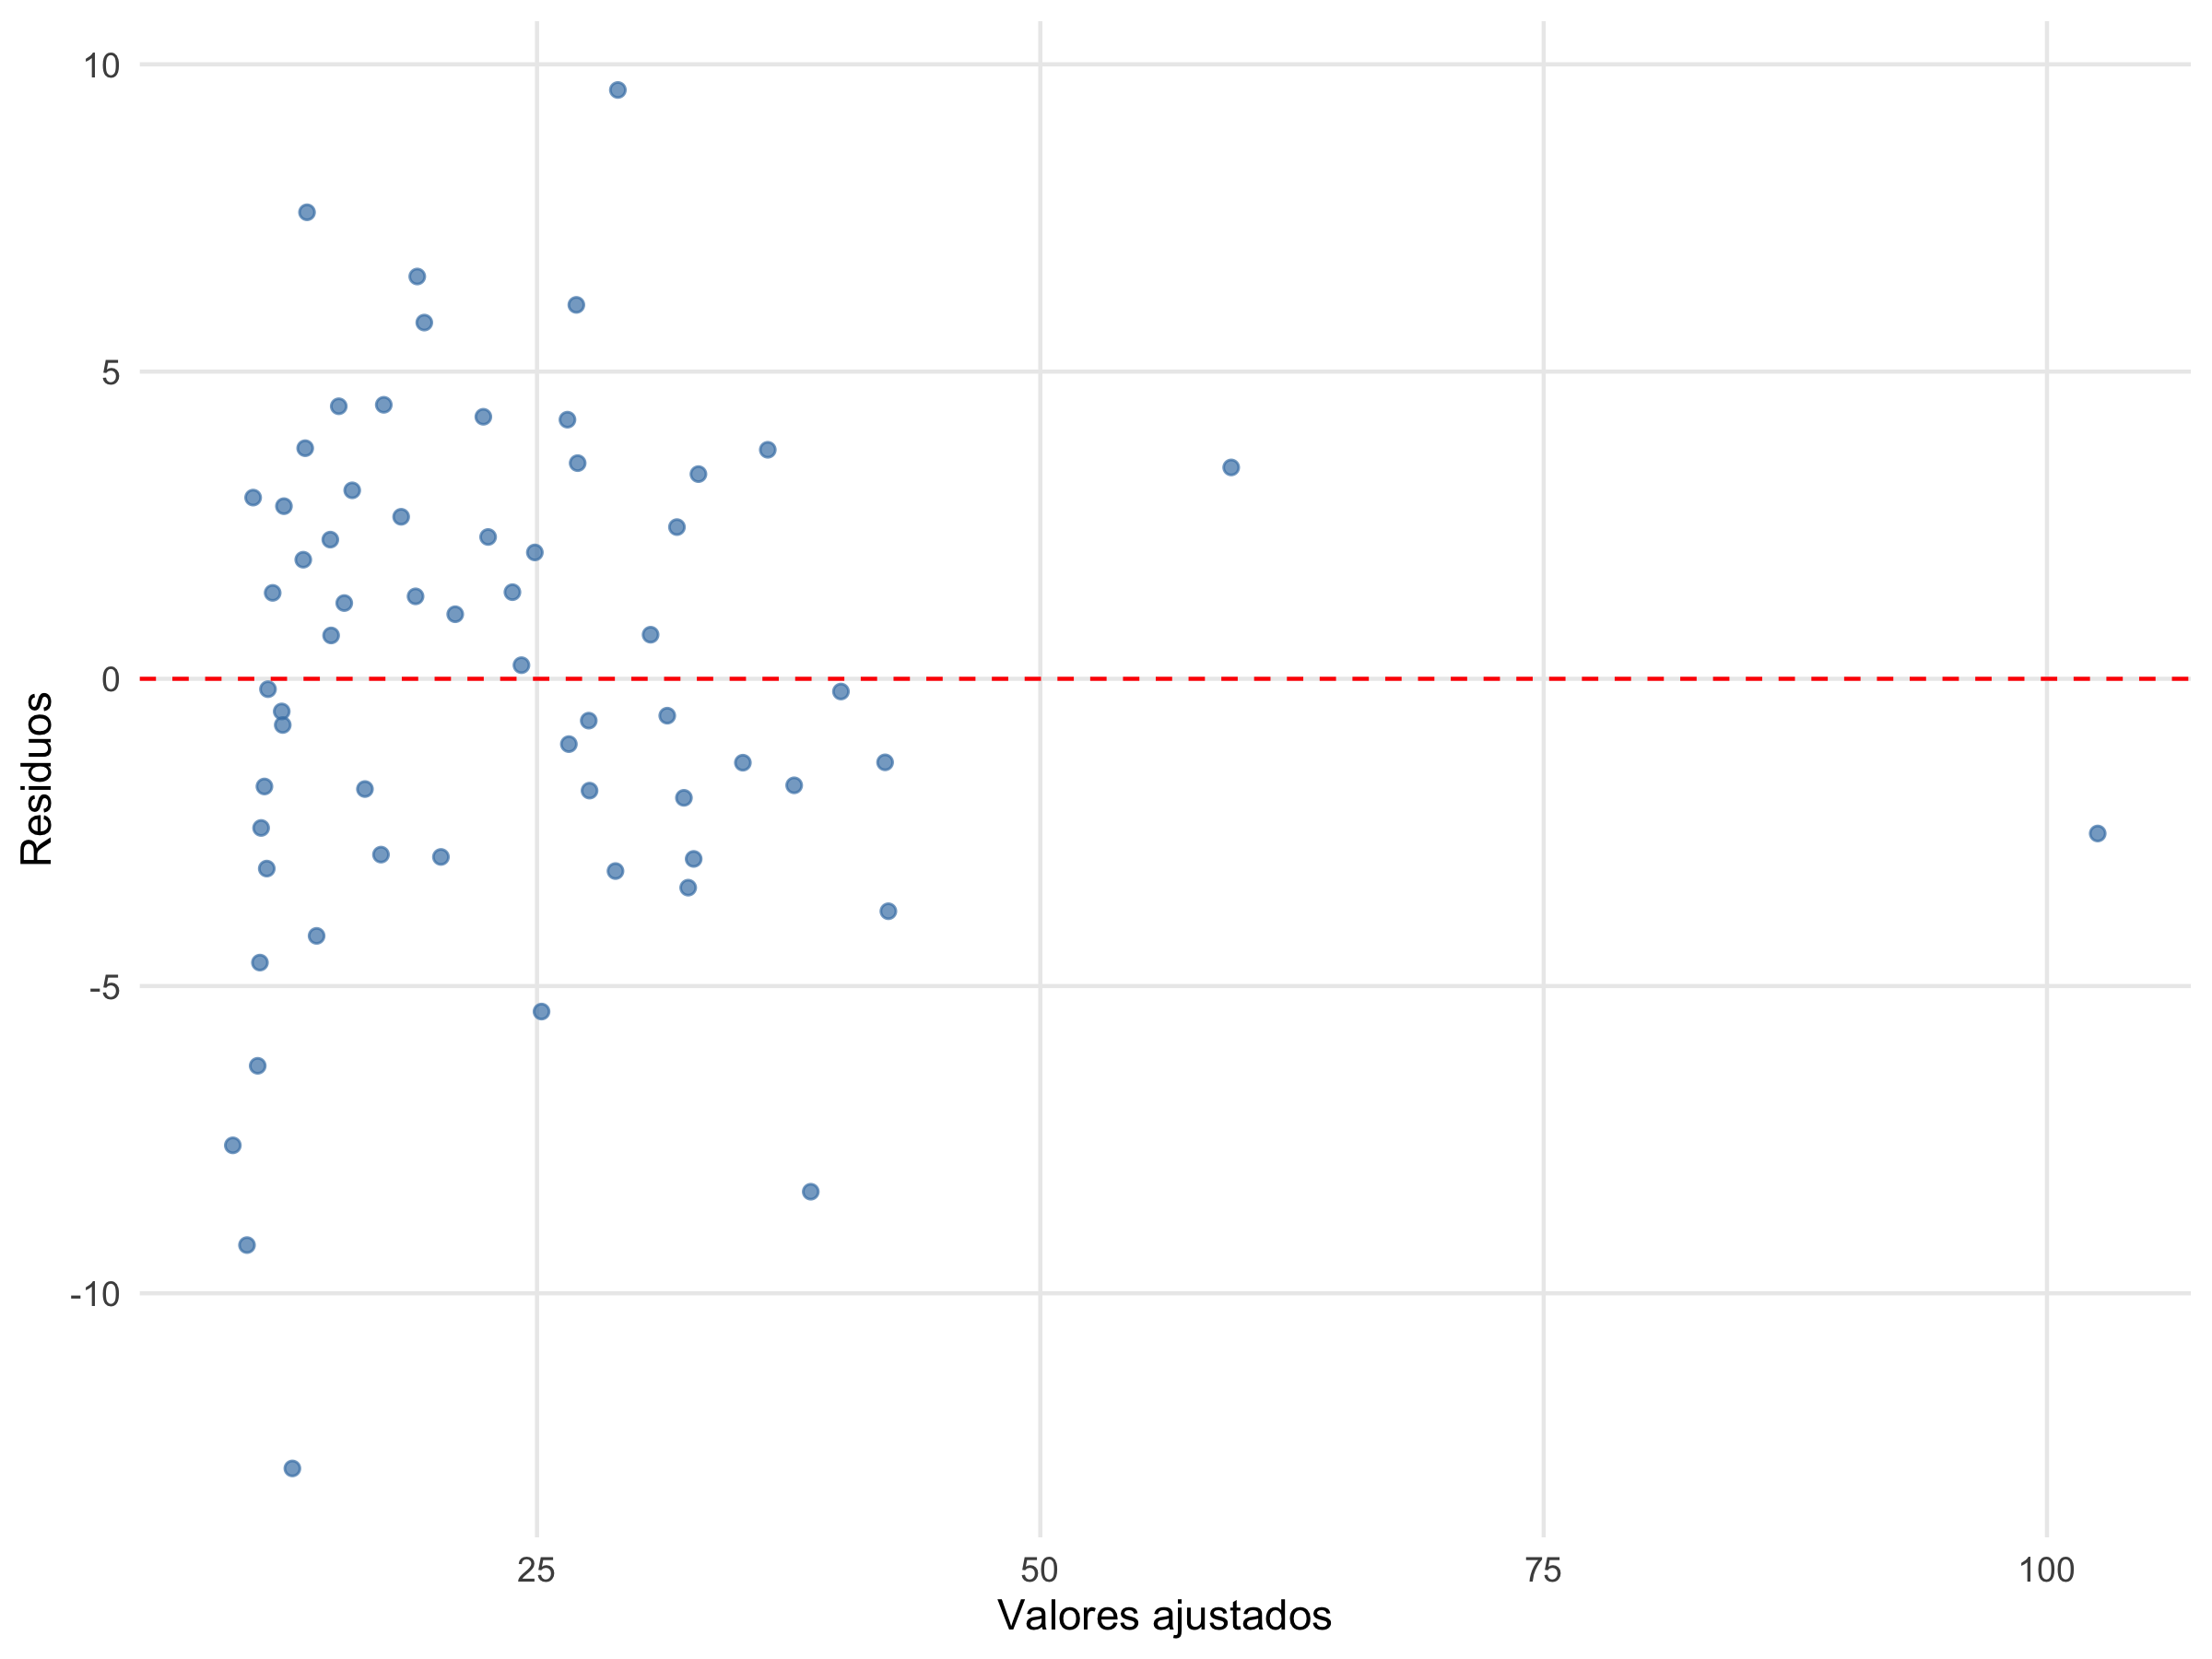
\includegraphics[width=\linewidth]{modelo_multip_residuos.png}
\end{center}
Figura 14. Dispersión de los residuos.




\begin{center}
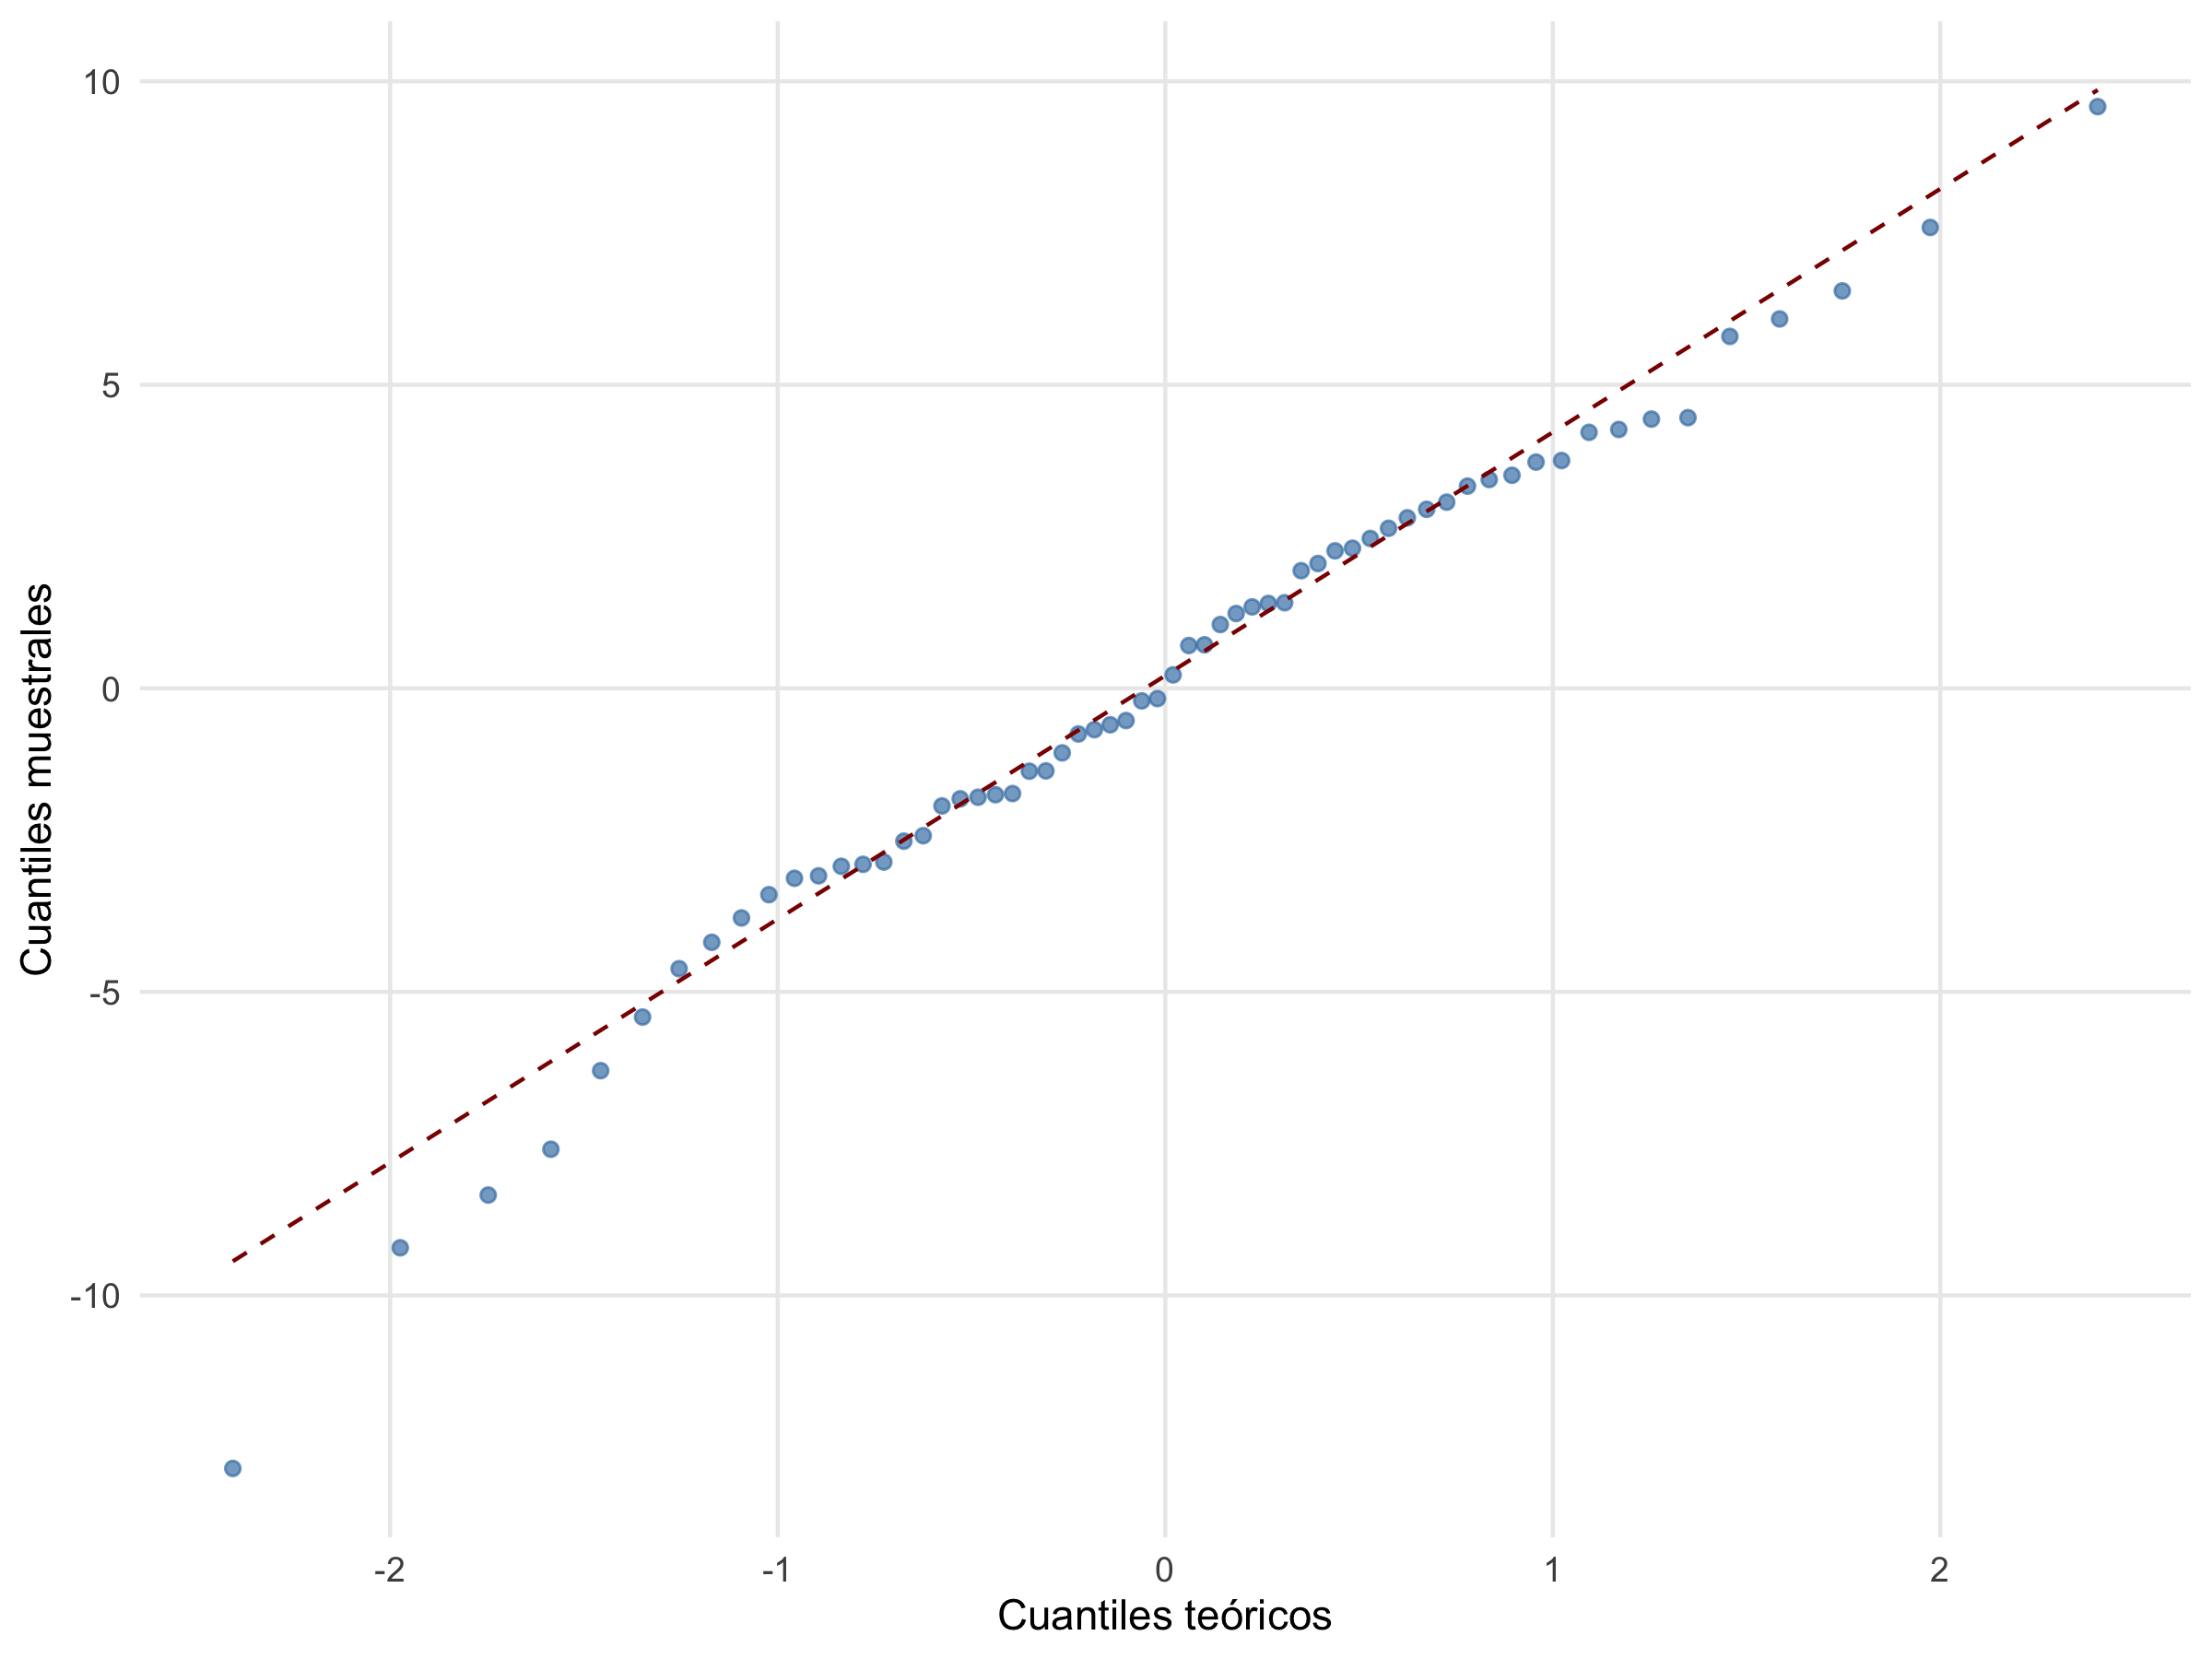
\includegraphics[width=\linewidth]{modelo_multip_normalidad.png}
\end{center}
Figura 15. Gráfico Q-Q.


\subsubsection*{Reflexión e interpretación}

Luego de verificar los supuestos y confirmar la significancia global del modelo, se analizó la influencia individual de cada variable independiente:

\begin{itemize}
  \item \textbf{Research} tuvo el mayor coeficiente, indicando que el desarrollo investigativo es el factor más determinante del Total Score.
  \item \textbf{Commerce} también resultó influyente, pero en menor magnitud.
  \item \textbf{Talent} fue significativo, mostrando que el capital humano también contribuye, aunque con un efecto más moderado.
\end{itemize}

\textbf{Recomendación:}  
Para mejorar el desempeño global en inteligencia artificial, los países deberían enfocar recursos en fortalecer sus capacidades de investigación. Este modelo puede emplearse para simular escenarios y priorizar políticas de inversión en los tres frentes analizados.

\section{Conclusiones}

Los datos analizados revelan una realidad preocupante: el avance de la inteligencia artificial no se distribuye de manera equitativa en el mundo. Al examinar factores clave como la inversión (Commerce), la innovación (Research) y la formación de especialistas (Talent), queda claro que solo un pequeño grupo de países —principalmente Estados Unidos, China y algunas potencias europeas— concentra la mayor parte del progreso en este campo.

Más del 60% de las naciones evaluadas muestra un rezago significativo en los tres aspectos estudiados, con regiones como África y América Latina en una posición particularmente vulnerable. Esta concentración no solo limita la capacidad competitiva de estas regiones, sino que las expone a una creciente dependencia tecnológica de los países más avanzados. Se requiere, por tanto, que los gobiernos implementen estrategias concretas para fomentar la investigación, atraer inversiones y formar profesionales altamente capacitados en IA.

El análisis mediante frecuencias univariadas y bivariadas de los tres indicadores clave revela patrones estructurales preocupantes. Se observa una concentración extrema de capacidades en un reducido grupo de países: Estados Unidos, con puntuaciones perfectas en Talent y Commerce, y China, destacada en Research con 71.42 puntos, lideran con una ventaja sustancial. Esta triple brecha —formativa, científica y comercial— se refleja en los valores acumulados, donde el 80% de los países presenta desempeños inferiores a los 30 puntos en los tres indicadores, lo cual genera un escenario crítico de dependencia y vulnerabilidad global.

El estudio también evidencia que solo el 12% de los países (7 de 58) alcanza simultáneamente puntuaciones altas (más de 70 puntos) en los tres indicadores, mientras que el 65% muestra limitaciones críticas en el índice Commerce (menos de 20 puntos). La brecha es particularmente grave en el índice Talent, donde Estados Unidos —con 100 puntos— quintuplica la media global (19.3 puntos), dejando en evidencia una concentración extrema del capital humano especializado.

Un punto relevante que debe considerarse es el posible sesgo estructural en los datos, especialmente en relación con Estados Unidos, que presenta valores extremos (máximos) en prácticamente todos los indicadores. Esta desproporción puede distorsionar la percepción del desarrollo relativo de los demás países, haciendo que sus desempeños se vean menos destacados en comparación. Este efecto se acentúa en los análisis de correlación y regresión, donde los valores atípicos influyen en los resultados agregados. Por tanto, futuros estudios deberían considerar técnicas de normalización o análisis por clusters regionales para evitar que un solo país —por más desarrollado que sea— defina las tendencias globales.

Finalmente, el estudio confirma que el éxito en inteligencia artificial no depende exclusivamente del Producto Interno Bruto. Factores como el compromiso político, la infraestructura digital, la calidad educativa y los marcos regulatorios tienen un peso determinante. Para cerrar la brecha, no basta con recursos financieros: se necesita visión estratégica, cooperación internacional y voluntad de democratizar el conocimiento. La IA no es solo una tecnología del futuro; es un reflejo de las desigualdades del presente. Democratizarla es, ante todo, un imperativo social.

\section{Referencias}
[1]   “AI Global Index,” Kaggle, Apr. 26, 2023.         https://www.kaggle.com/datasets/katerynameleshenko/ai-index

[2]   W. Navidi, Statistics for Engineers and Scientists w/ CD-ROM. McGraw-Hill Sci./Eng./Math, 2004.

[3] Academia Lab, "Teorema del límite central," Enciclopedia, 2025. [Online]. Available: https://academia-lab.com/enciclopedia/teorema-del-limite-central/. [Accessed: May 16, 2025].

[4] Minitab, "¿Qué es un valor crítico?," Minitab Support, 2025. [Online]. Available: https://support.minitab.com/es-mx/minitab/help-and-how-to/statistics/basic-statistics/supporting-topics/basics/what-is-a-critical-value/. [Accessed: May 16, 2025].

[5] Universidad de los Andes, "Regresión lineal: qué es y cómo funciona," Programas Uniandes, 2025. [Online]. Available: https://programas.uniandes.edu.co/blog/regresion-lineal. [Accessed: May 16, 2025].

[6] D. Diez, M. Çetinkaya-Rundel, and C. Barr, OpenIntro Statistics: Fourth Edition. OpenIntro, Inc., 2019.


\end{multicols}

\end{document}
